\documentclass{assignment}
\usepackage[pdftex]{graphicx} 
\usepackage{xcolor}
\definecolor{LightGray}{gray}{0.95}
%\usepackage{fancyvrb, minted} 
\usepackage[a4paper, margin = 2.5cm]{geometry} 
\usepackage[T1]{fontenc} 
% set figure path 
\graphicspath{figures}

\usepackage{amsmath, amsfonts, amssymb} 
\usepackage{hyperref, url}  
\usepackage{fancyhdr}
\usepackage{setspace}
\onehalfspacing

\usepackage{float}
\usepackage{subcaption}
\usepackage{listingsutf8}

\usepackage{xcolor}

\definecolor{codegreen}{rgb}{0,0.6,0}
\definecolor{codegray}{rgb}{0.5,0.5,0.5}
\definecolor{codepurple}{rgb}{0.58,0,0.82}
\definecolor{backcolour}{rgb}{0.95,0.95,0.92}

\lstdefinestyle{mystyle}{
    backgroundcolor=\color{backcolour},   
    commentstyle=\color{codegreen},
    keywordstyle=\color{magenta},
    numberstyle=\tiny\color{codegray},
    stringstyle=\color{codepurple},
    basicstyle=\ttfamily\footnotesize,
    breakatwhitespace=false,         
    breaklines=true,                 
    captionpos=b,                    
    keepspaces=true,                 
    numbers=left,                    
    numbersep=5pt,                  
    showspaces=false,                
    showstringspaces=false,
    showtabs=false,                  
    tabsize=2
}

\lstset{style=mystyle}

\student{Ahmet Akman 2442366}                             
\semester{Spring 2024}                            
\date{\today}                                   

\courselabel{EE449}          
\exercisesheet{Homework 3}{Report}  

\school{Middle East Technical University}        
\university{Electrical and Electronics Engineering}        

%%%%%%%%%%%%%%%%%%%%%%%%%%%%%%%%%%%%%%%%%%-DOCUMENT-%%%%%%%%%%%%%%%%%%%%%%%%%%%%%%%%%%%%%%%%%%%%

\begin{document}
\section{Questions}
\subsection{Agent: }
Agent corresponds to the entity that interacts with the environment. It is responsible for taking actions, observing the environment, and receiving rewards. The agent is the entity that learns the optimal policy to maximize the cumulative reward. When compared to supervised learning, the agent is not provided with the correct output, but it learns the optimal policy through trial and error. That is concept of error is not exactly available in reinforcement setting.

\subsection{Environment: }
Environment means the world that the agent interacts with. It is the entity that the agent observes and takes actions. The environment is responsible for providing the agent with the current state, reward, and possible actions. The environment is also responsible for updating the state of the agent based on the action taken by the agent. When compared to supervised learning, the environment corresponds to the both dataset and loss function that the system trained and run on.

\subsection{Reward: }
Reward is the feedback that the agent receives from the environment. It is the scalar value that the agent receives after taking an action. The reward is used to evaluate the action taken by the agent. The agent aims to maximize the cumulative reward by learning the optimal policy. When compared to supervised learning, the reward corresponds to the loss function that the system tries to minimize.

\subsection{Policy: }
Policy is the strategy that the agent uses to take actions. It is the mapping from the state to the action. If we compare with supervised learning, the policy corresponds to the model that the system uses to predict the output.

\subsection{Exploration: }
The exploration corresponds to the process of trying different actions to learn the optimal policy. The agent explores the environment by taking different actions and observing the reward. The exploration is necessary to learn the optimal policy. When we try to map exploration to supervised learning step we may encounter more than one phenomena. For example, we can say that exploration corresponds to the training process of the model. On the other hand we can say the exploration corresponds to the data augmentation process or other randomization steps taken during training.

\subsection{Exploitation: }
Exploitation corresponds to the process of taking the best action based on the learned policy. The agent exploits the environment by taking the action that maximizes the reward. The exploitation is necessary to maximize the cumulative reward. When we try to map exploitation to supervised learning step, we can say that exploitation corresponds to the inference process of the model. 

\section{Experimental Work}
The proper implementation for maze, temporal difference learning and Q-learning are implemented and provided in appendix. 

\noindent The experimental work section is divided into four main part where each part has TD learning and Q learning related experiments seperately. First the default parameter outputs are presented. Then the effect of alpha parameter is investigated. After that the effect of gamma parameter is investigated. Lastly the effect of epsilon parameter is investigated.
\subsection{Temporal Difference Learning Default Parameters}
The default parameters for the temporal difference learning are set as follows:
\begin{itemize}
    \item Alpha: 0.1
    \item Gamma: 0.95
    \item Epsilon: 0.2
    \item Episodes: 10000
\end{itemize}
According to these settings the training is done. The policy maps are provided  in Figure \ref{fig:default_td_learning_policy}. The value function plots are provided in Figure \ref{fig:default_td_learning_value}. The convergence plots are provided in Figure \ref{fig:default_td_learning_convergence}.

Basically we can say that the agent learns the optimal policy and value function.

% polict map plots
\begin{figure}[H]
    \begin{subfigure}{0.3\textwidth}
        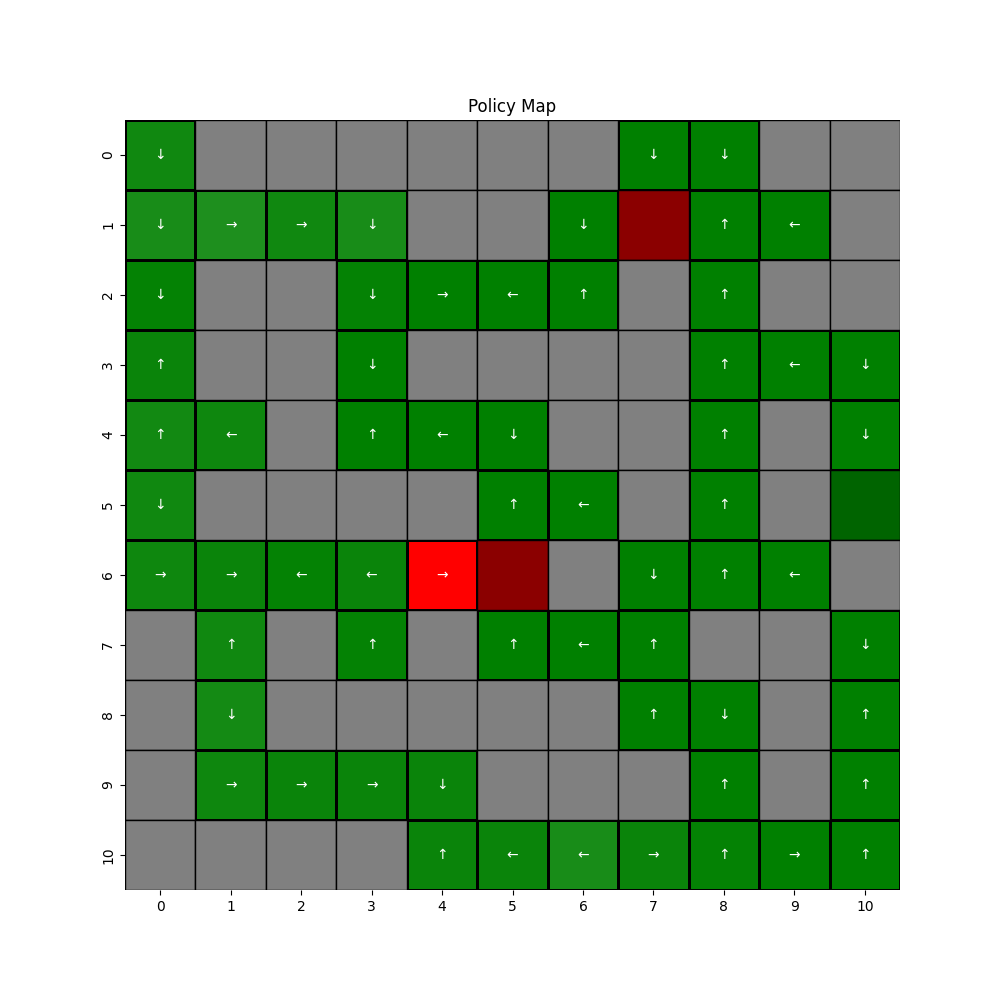
\includegraphics[width=\textwidth]{figures/policy_td/default/policy_alpha_0.1_gamma_0.95_epsilon_0.2_iteration_1.png}
    \caption{Episode 1.}
    \end{subfigure}\hfill
    \begin{subfigure}{0.3\textwidth}
        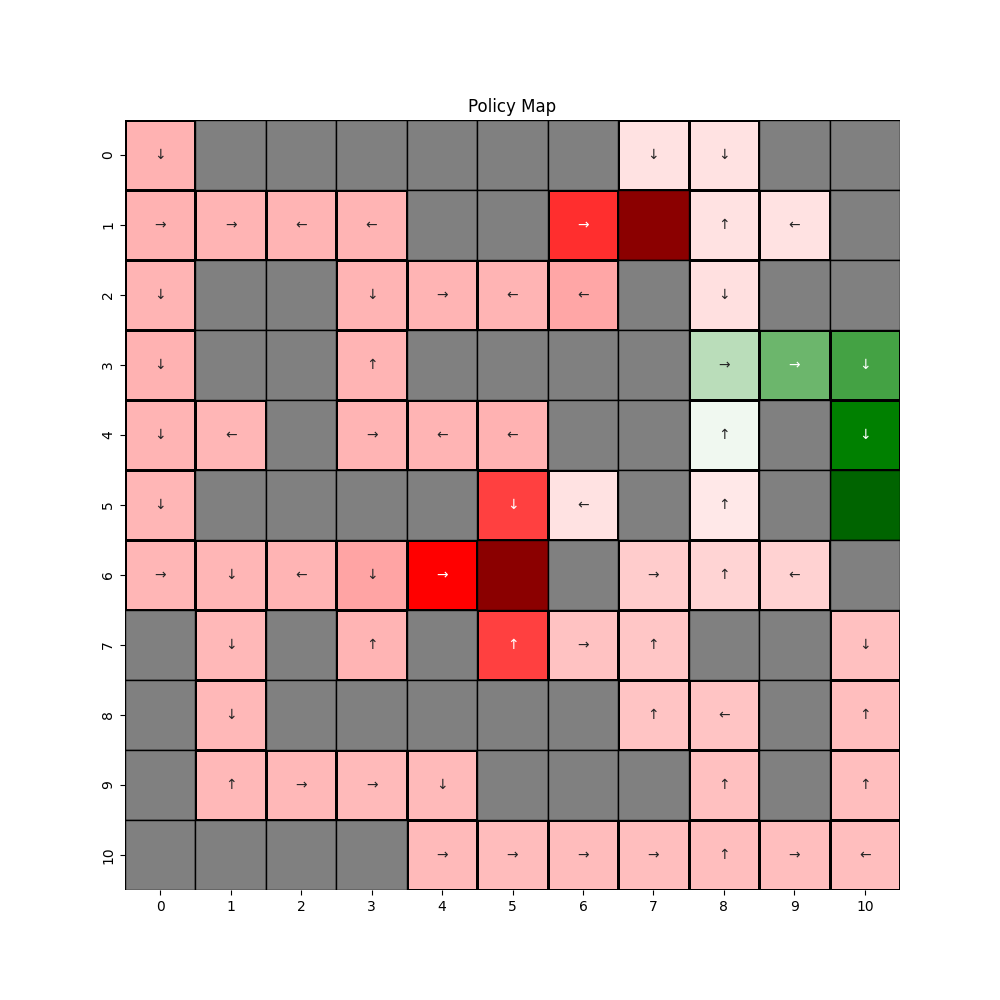
\includegraphics[width=\textwidth]{figures/policy_td/default/policy_alpha_0.1_gamma_0.95_epsilon_0.2_iteration_50.png}
    \caption{Episode 50}
    \end{subfigure}\hfill
    \begin{subfigure}{0.3\textwidth}
        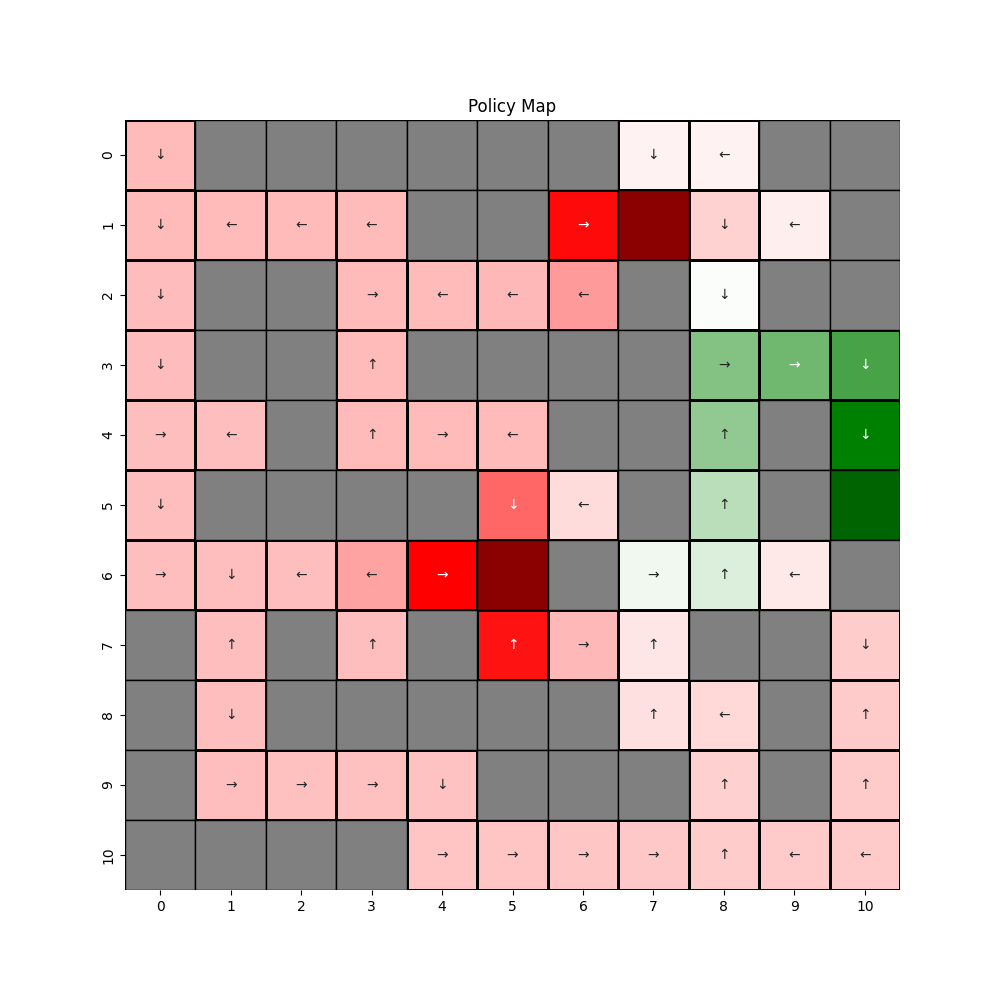
\includegraphics[width=\textwidth]{figures/policy_td/default/policy_alpha_0.1_gamma_0.95_epsilon_0.2_iteration_100.png}
    \caption{Episode 100}
    \end{subfigure}
    \begin{subfigure}{0.3\textwidth}
        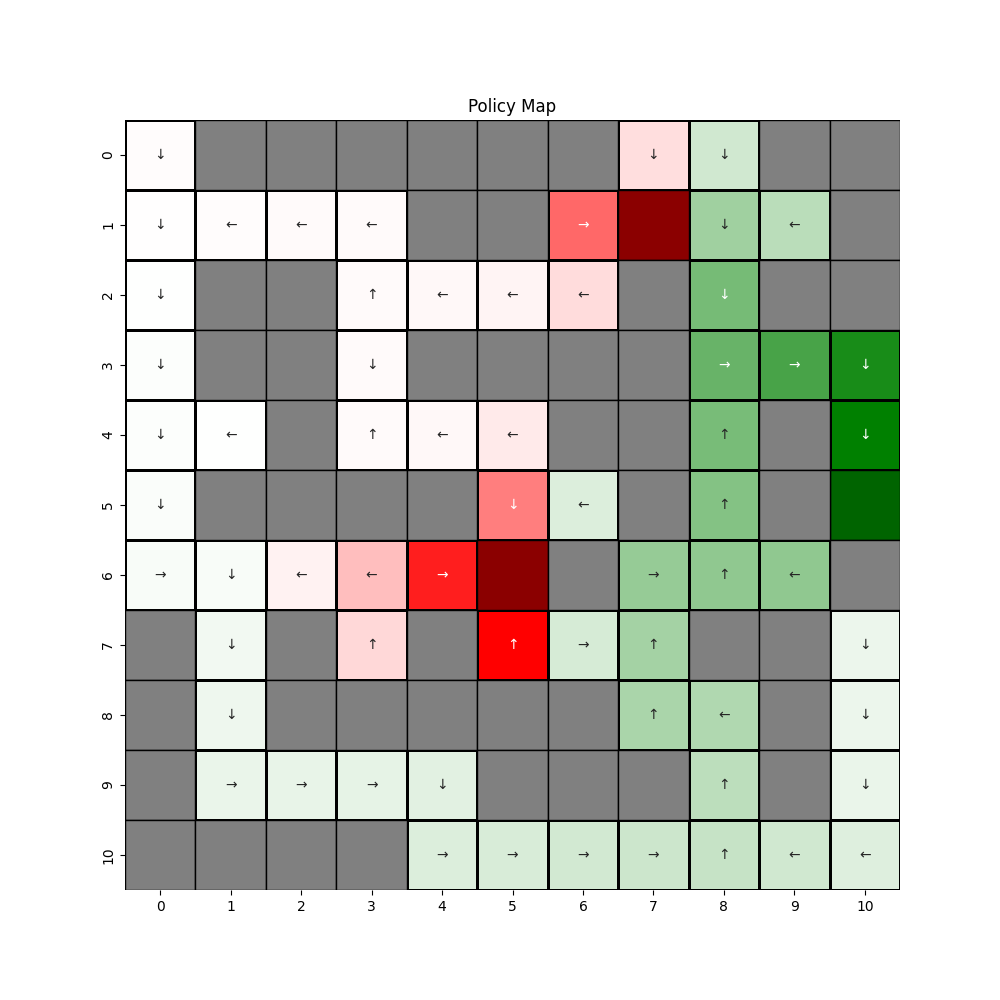
\includegraphics[width=\textwidth]{figures/policy_td/default/policy_alpha_0.1_gamma_0.95_epsilon_0.2_iteration_1000.png}
    \caption{Episode 1000.}
    \end{subfigure}\hfill
    \begin{subfigure}{0.3\textwidth}
        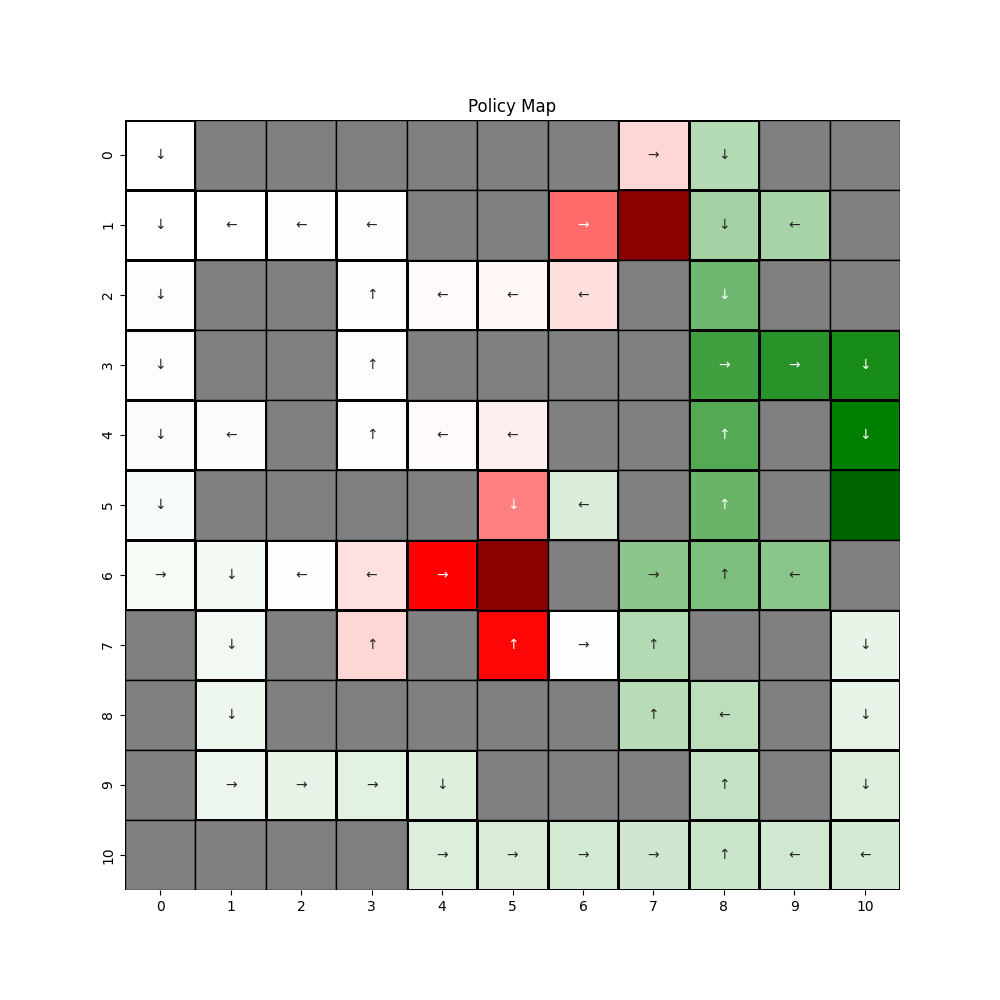
\includegraphics[width=\textwidth]{figures/policy_td/default/policy_alpha_0.1_gamma_0.95_epsilon_0.2_iteration_5000.png}
    \caption{Episode 5000}
    \end{subfigure}\hfill
    \begin{subfigure}{0.3\textwidth}
        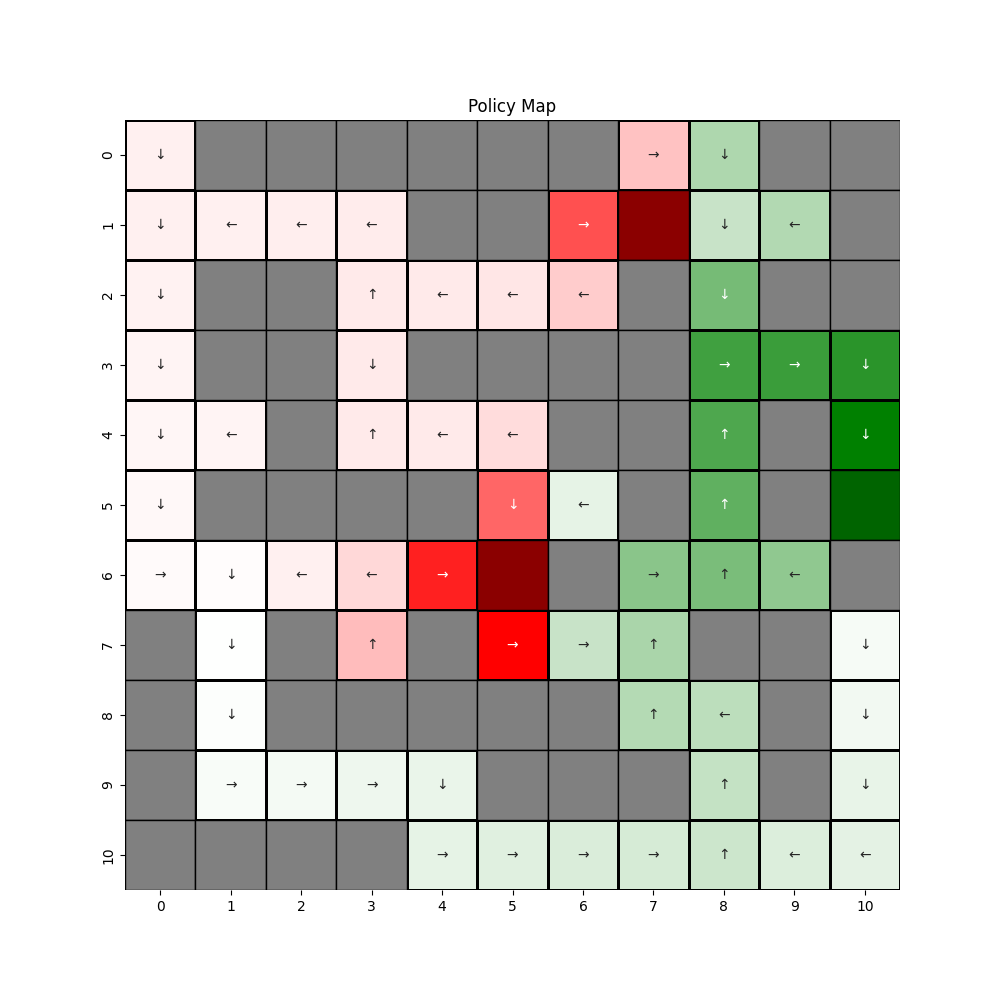
\includegraphics[width=\textwidth]{figures/policy_td/default/policy_alpha_0.1_gamma_0.95_epsilon_0.2_iteration_10000.png}
    \caption{Episode 10000}
    \end{subfigure}
    \caption{Evolution of policy maps throughout episodes.}
    \label{fig:default_td_learning_policy}
\end{figure}

% value function plots

\begin{figure}[H]
    \begin{subfigure}{0.3\textwidth}
        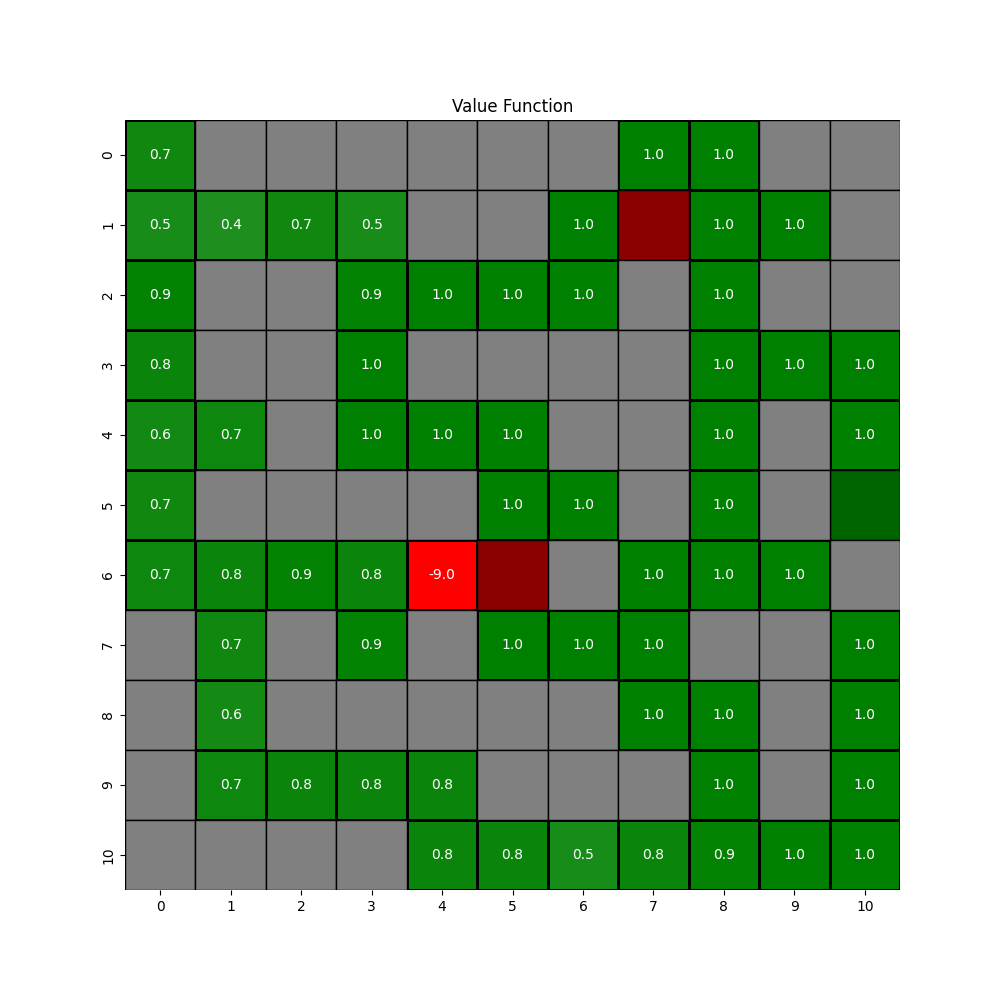
\includegraphics[width=\textwidth]{figures/value_td/default/value_function_alpha_0.1_gamma_0.95_epsilon_0.2_iteration_1.png}
    \caption{Episode 1.}
    \end{subfigure}\hfill
    \begin{subfigure}{0.3\textwidth}
        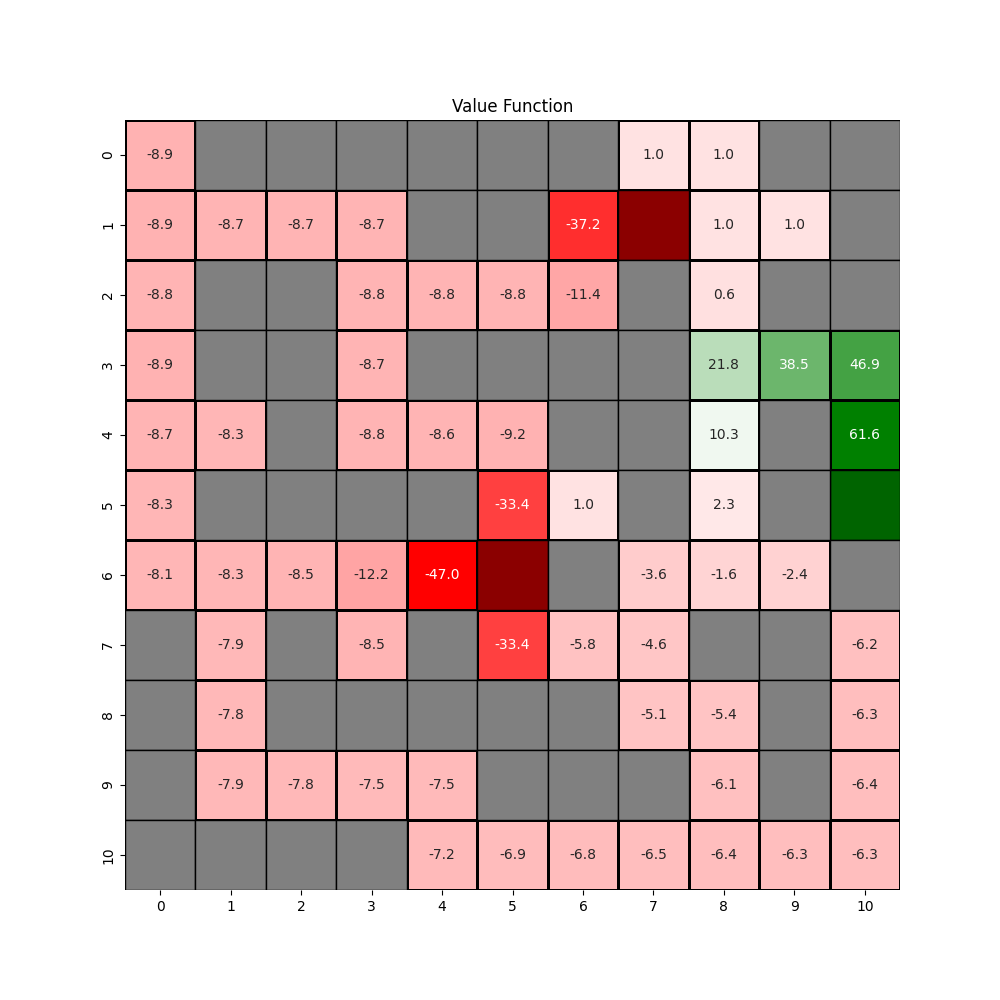
\includegraphics[width=\textwidth]{figures/value_td/default/value_function_alpha_0.1_gamma_0.95_epsilon_0.2_iteration_50.png}
    \caption{Episode 50}
    \end{subfigure}\hfill
    \begin{subfigure}{0.3\textwidth}
        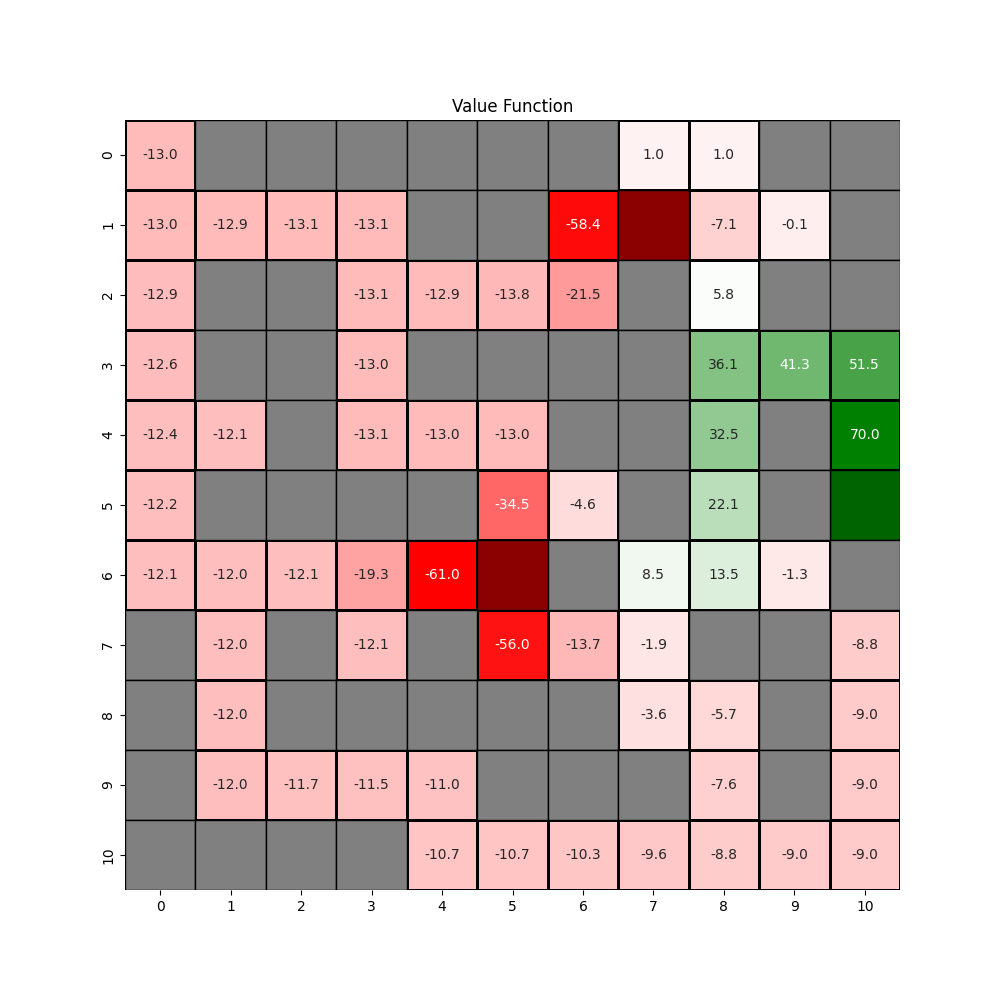
\includegraphics[width=\textwidth]{figures/value_td/default/value_function_alpha_0.1_gamma_0.95_epsilon_0.2_iteration_100.png}
    \caption{Episode 100}
    \end{subfigure}
    \begin{subfigure}{0.3\textwidth}
        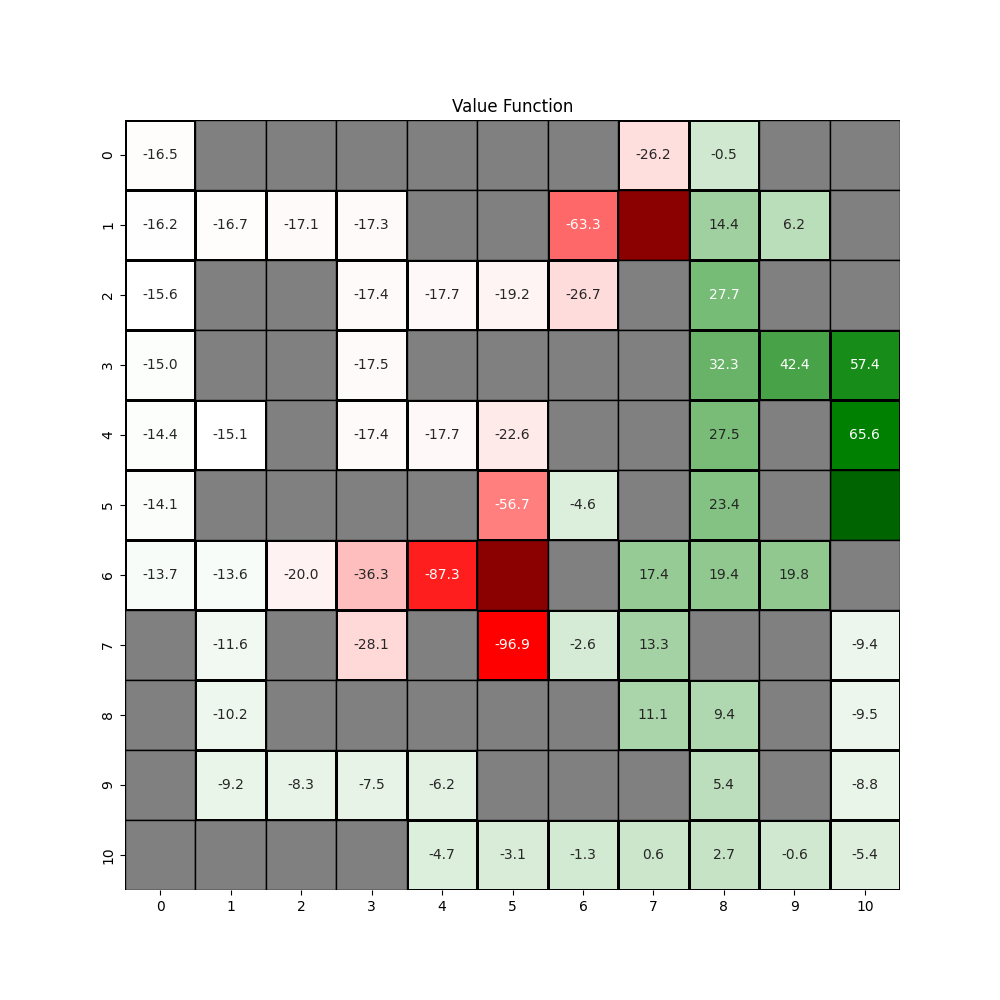
\includegraphics[width=\textwidth]{figures/value_td/default/value_function_alpha_0.1_gamma_0.95_epsilon_0.2_iteration_1000.png}
    \caption{Episode 1000.}
    \end{subfigure}\hfill
    \begin{subfigure}{0.3\textwidth}
        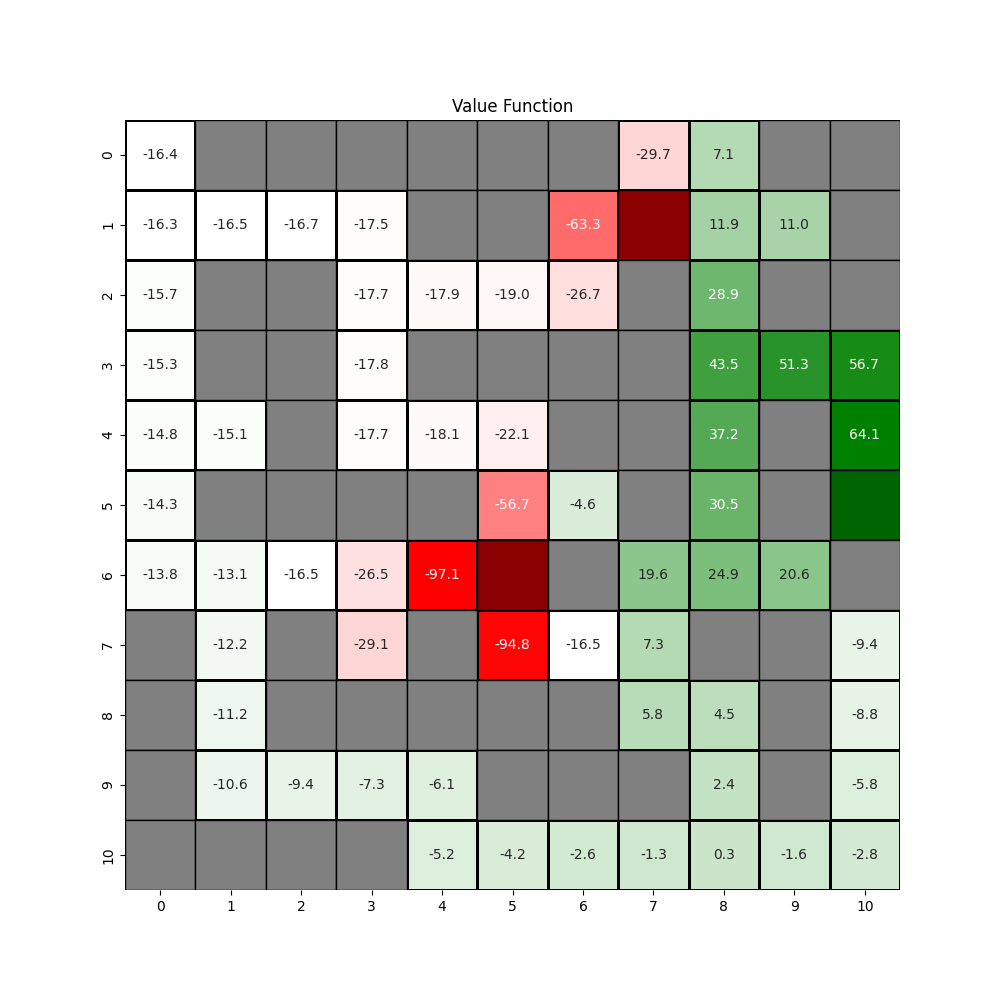
\includegraphics[width=\textwidth]{figures/value_td/default/value_function_alpha_0.1_gamma_0.95_epsilon_0.2_iteration_5000.png}
    \caption{Episode 5000}
    \end{subfigure}\hfill
    \begin{subfigure}{0.3\textwidth}
        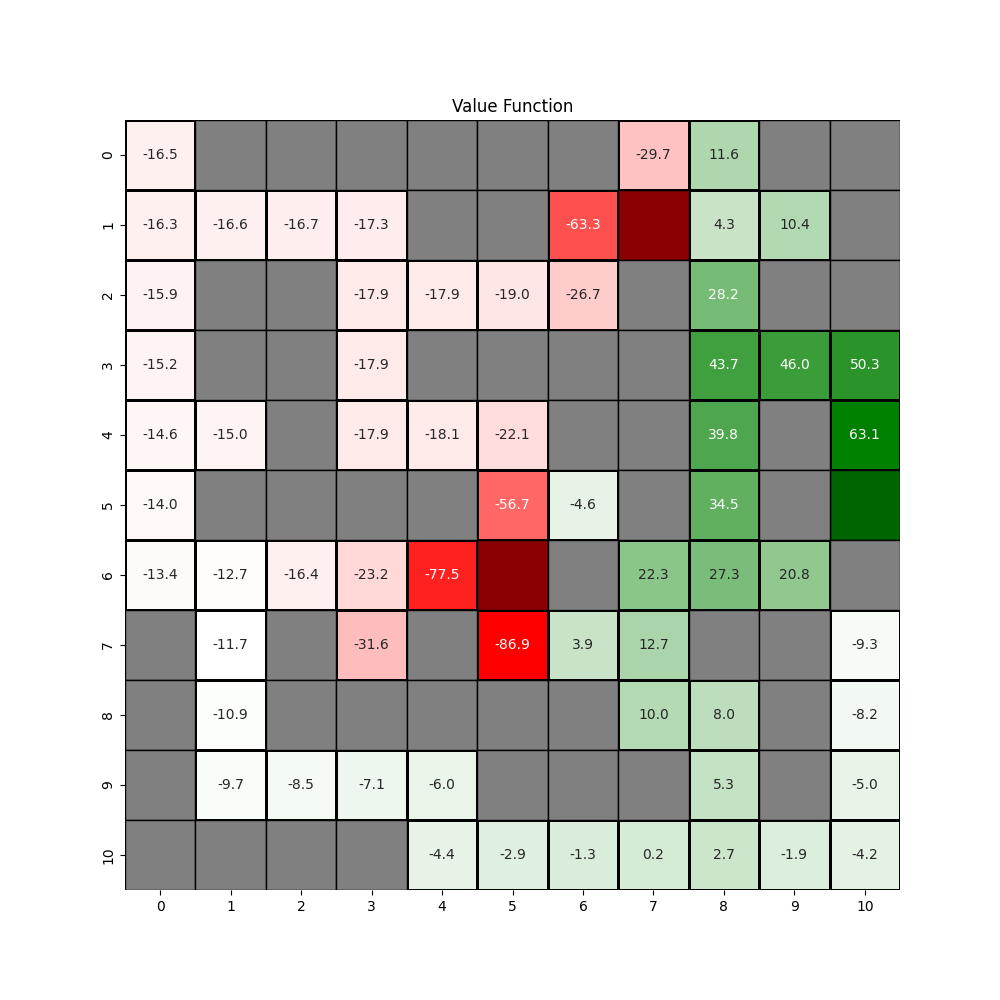
\includegraphics[width=\textwidth]{figures/value_td/default/value_function_alpha_0.1_gamma_0.95_epsilon_0.2_iteration_10000.png}
    \caption{Episode 10000}
    \end{subfigure}
    \caption{Evolution of value function throughout episodes.}
    \label{fig:default_td_learning_value}
\end{figure}

% convergence plots

\begin{figure}[H]
    \begin{subfigure}{0.5\textwidth}
        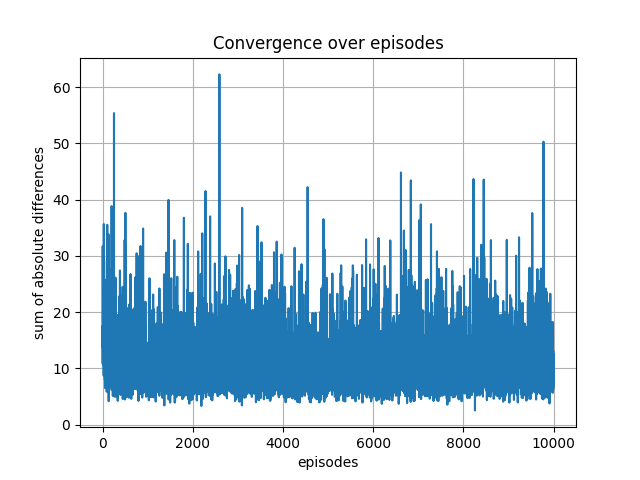
\includegraphics[width=\textwidth]{figures/convergence_td/default/convergence_TD_alpha_0.1_gamma_0.95_epislon_0.2.png}
    \caption{Converge raw.}
    \end{subfigure}\hfill
    \begin{subfigure}{0.5\textwidth}
        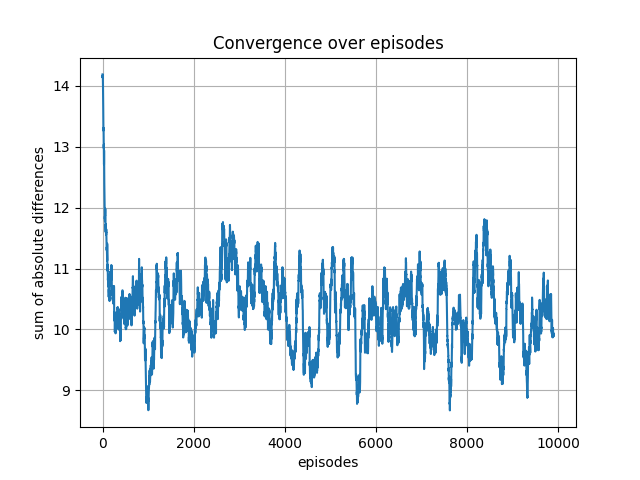
\includegraphics[width=\textwidth]{figures/convergence_td/default/convergence_TD_smoothed_alpha_0.1_gamma_0.95_epislon_0.2.png}
    \caption{Smoothed convergence.}
    \end{subfigure}
    \caption{Converge of value function.}
    \label{fig:default_td_learning_convergence}
\end{figure}





\subsection{Q-Learning Default Parameters}
As same as the temporal difference learning, the default parameters for the Q-learning are set. Then the training is done. The policy maps are provided  in Figure \ref{fig:default_q_learning_policy}. The value function plots are provided in Figure \ref{fig:default_q_learning_value}. The convergence plots are provided in Figure \ref{fig:default_q_learning_convergence}.

So, again we can say that the agent learns the optimal policy and value function at the end.

% polict map plots
\begin{figure}[H]
    \begin{subfigure}{0.3\textwidth}
        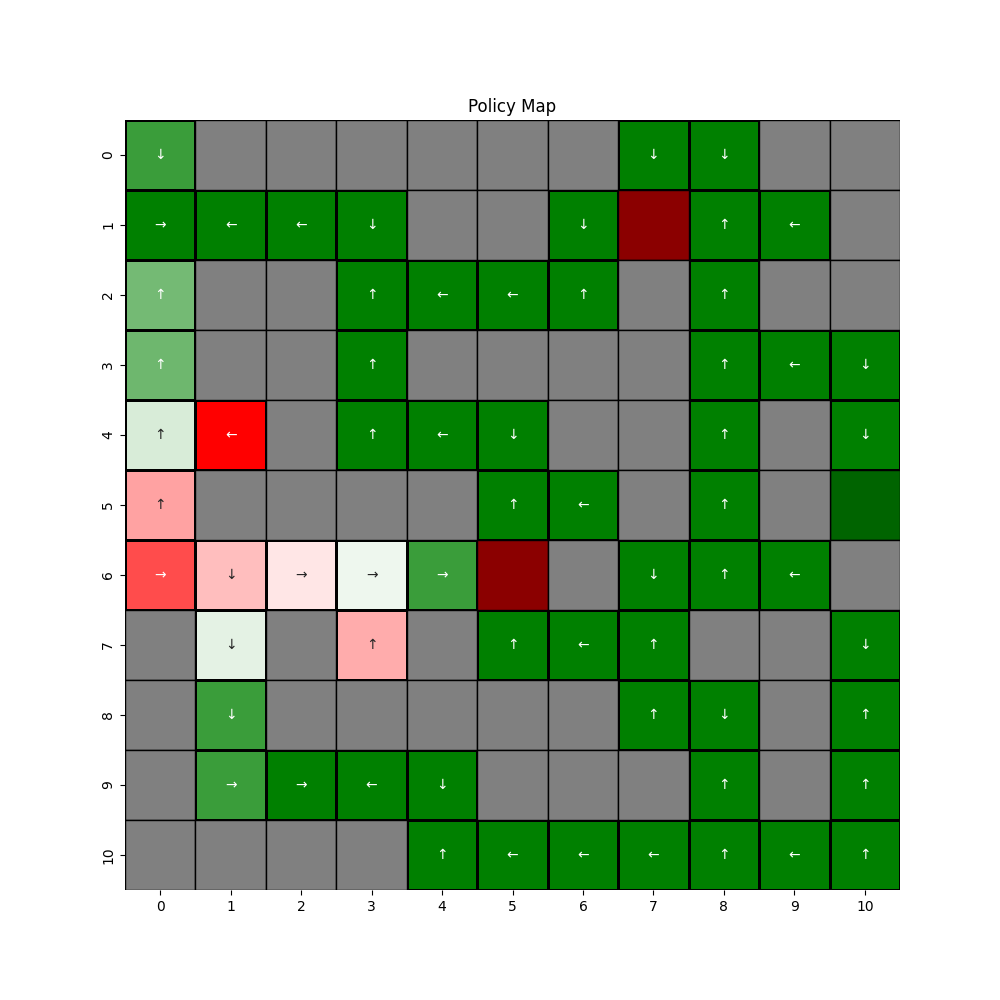
\includegraphics[width=\textwidth]{figures/policy_q/default/policy_alpha_0.1_gamma_0.95_epsilon_0.2_iteration_1.png}
    \caption{Episode 1.}
    \end{subfigure}\hfill
    \begin{subfigure}{0.3\textwidth}
        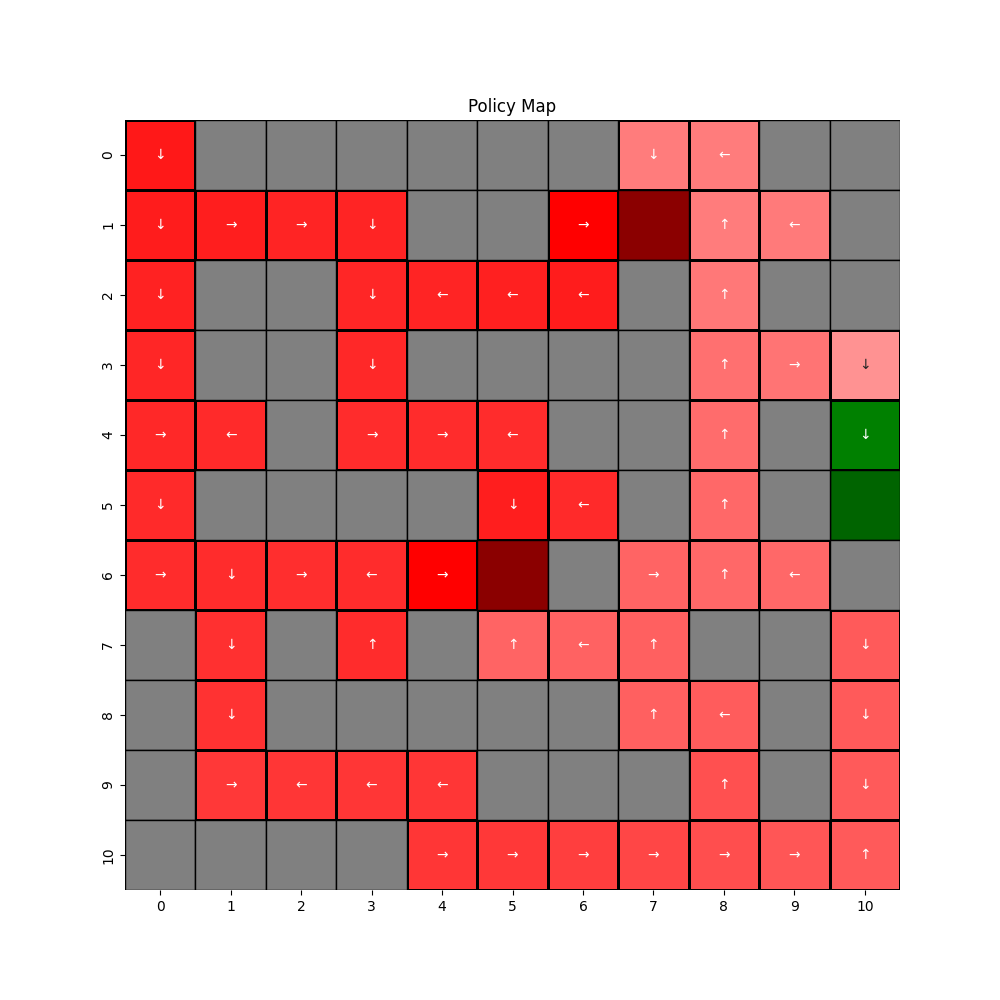
\includegraphics[width=\textwidth]{figures/policy_q/default/policy_alpha_0.1_gamma_0.95_epsilon_0.2_iteration_50.png}
    \caption{Episode 50}
    \end{subfigure}\hfill
    \begin{subfigure}{0.3\textwidth}
        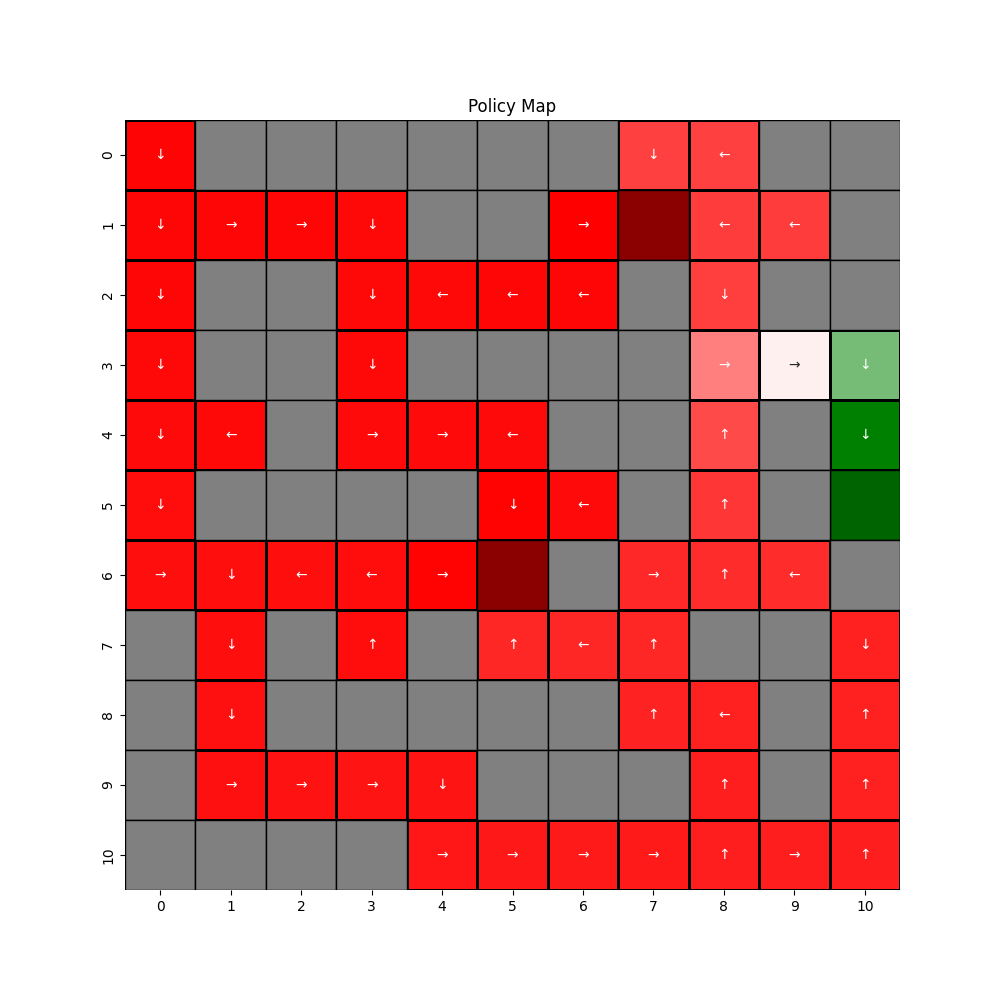
\includegraphics[width=\textwidth]{figures/policy_q/default/policy_alpha_0.1_gamma_0.95_epsilon_0.2_iteration_100.png}
    \caption{Episode 100}
    \end{subfigure}
    \begin{subfigure}{0.3\textwidth}
        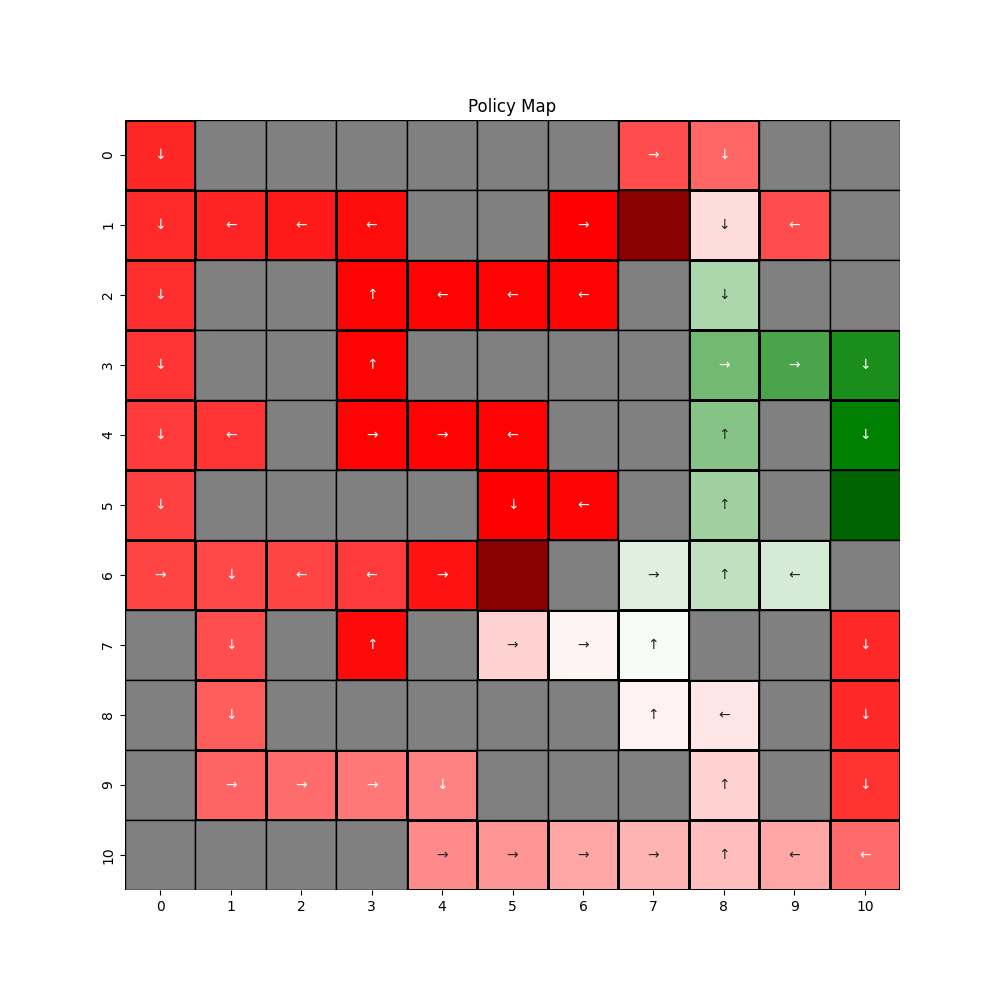
\includegraphics[width=\textwidth]{figures/policy_q/default/policy_alpha_0.1_gamma_0.95_epsilon_0.2_iteration_1000.png}
    \caption{Episode 1000.}
    \end{subfigure}\hfill
    \begin{subfigure}{0.3\textwidth}
        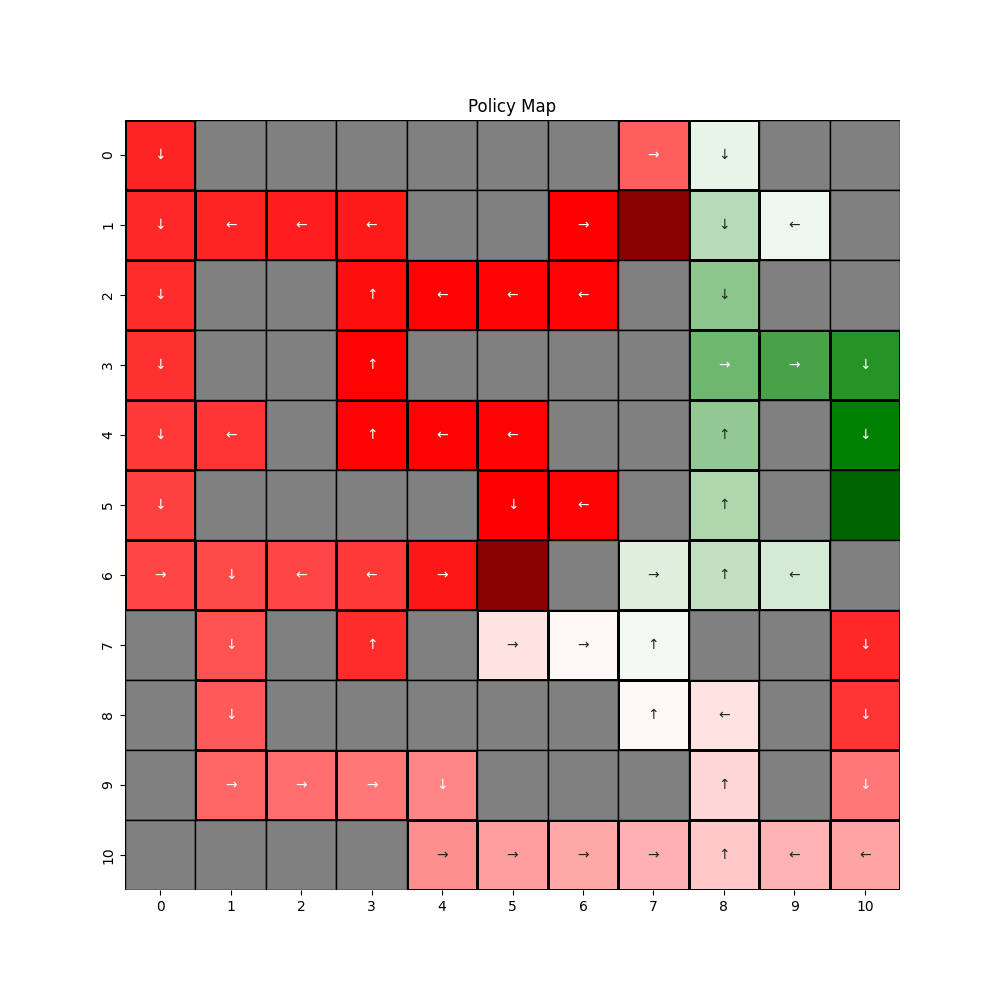
\includegraphics[width=\textwidth]{figures/policy_q/default/policy_alpha_0.1_gamma_0.95_epsilon_0.2_iteration_5000.png}
    \caption{Episode 5000}
    \end{subfigure}\hfill
    \begin{subfigure}{0.3\textwidth}
        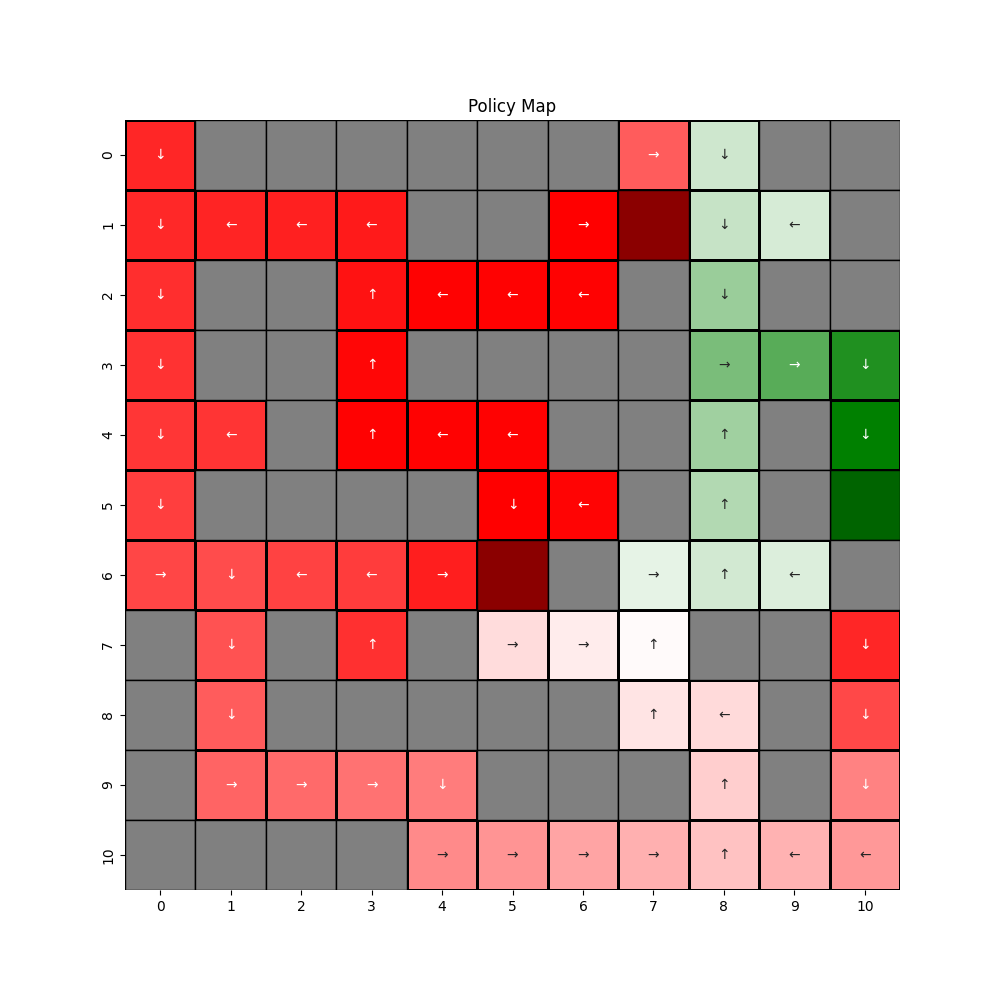
\includegraphics[width=\textwidth]{figures/policy_q/default/policy_alpha_0.1_gamma_0.95_epsilon_0.2_iteration_10000.png}
    \caption{Episode 10000}
    \end{subfigure}
    \caption{Evolution of policy maps throughout episodes.}
    \label{fig:default_q_learning_policy}
\end{figure}



% value function plots
\begin{figure}[H]
    \begin{subfigure}{0.3\textwidth}
        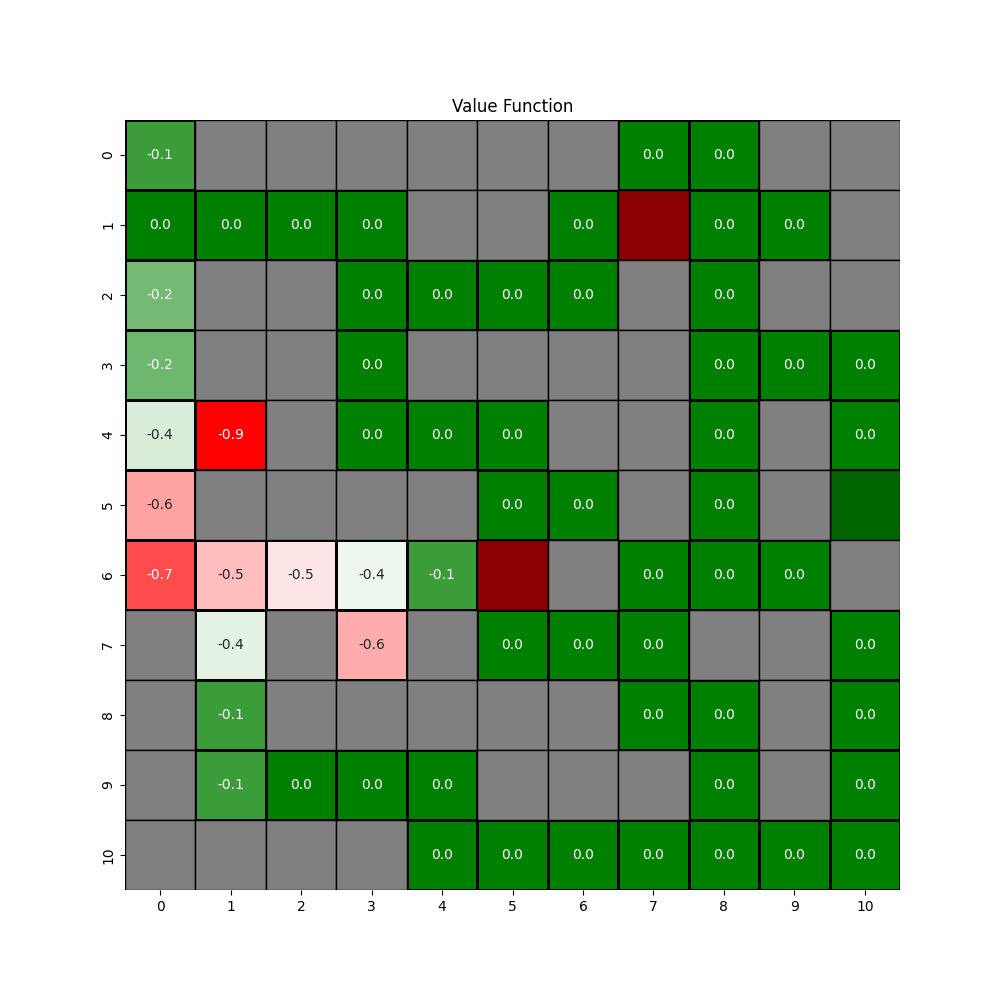
\includegraphics[width=\textwidth]{figures/value_q/default/value_function_alpha_0.1_gamma_0.95_epsilon_0.2_iteration_1.png}
    \caption{Episode 1.}
    \end{subfigure}\hfill
    \begin{subfigure}{0.3\textwidth}
        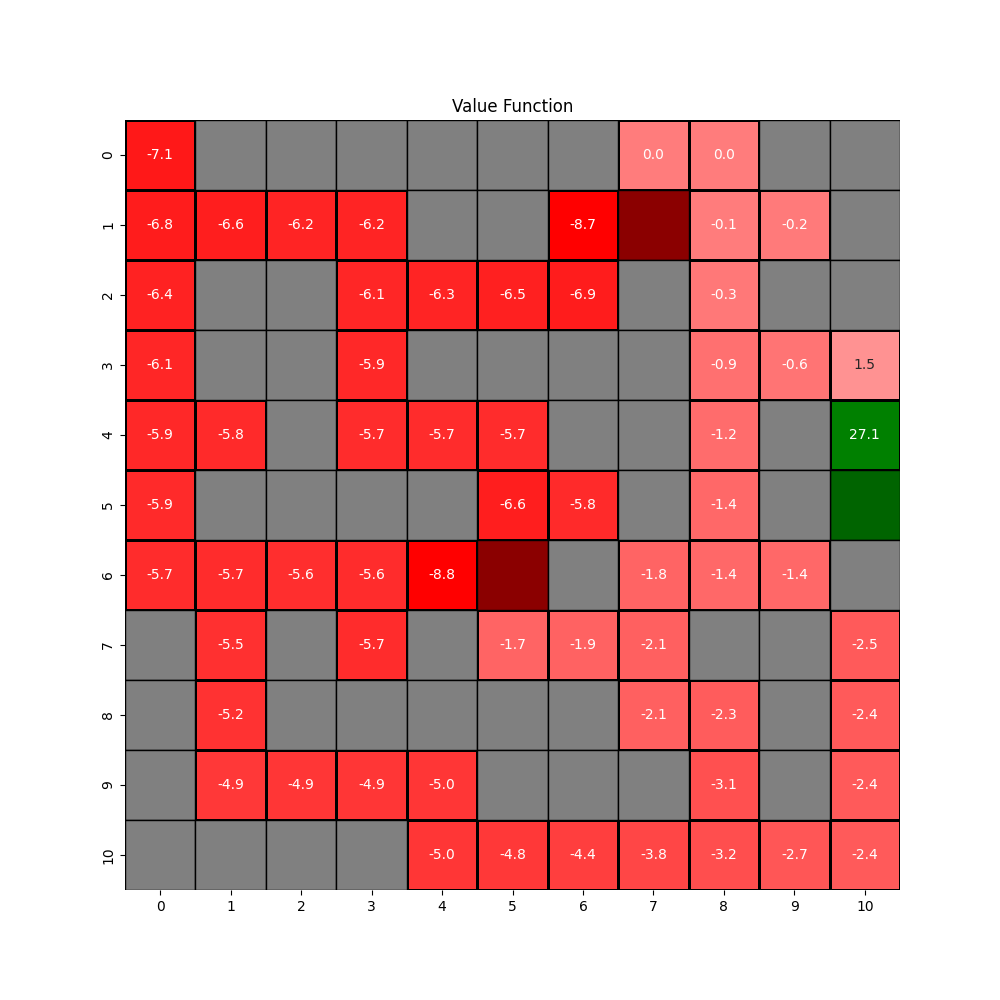
\includegraphics[width=\textwidth]{figures/value_q/default/value_function_alpha_0.1_gamma_0.95_epsilon_0.2_iteration_50.png}
    \caption{Episode 50}
    \end{subfigure}\hfill
    \begin{subfigure}{0.3\textwidth}
        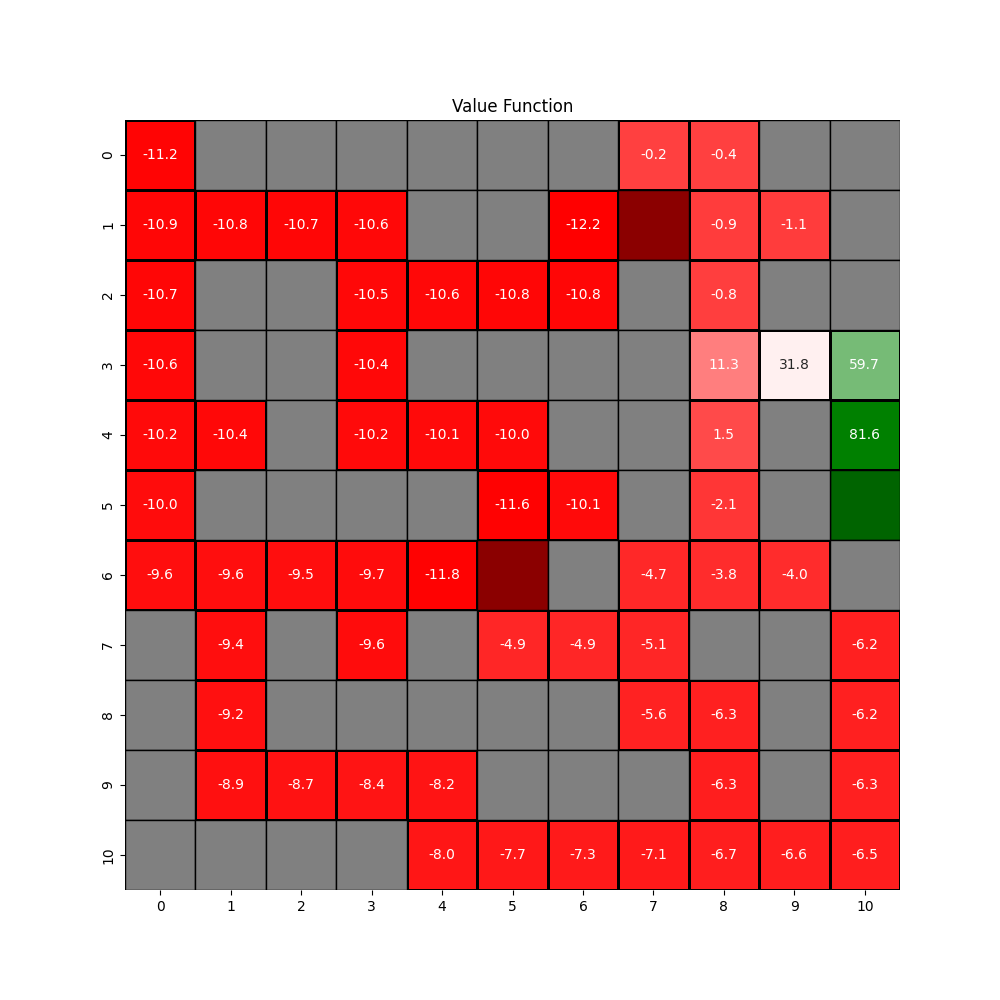
\includegraphics[width=\textwidth]{figures/value_q/default/value_function_alpha_0.1_gamma_0.95_epsilon_0.2_iteration_100.png}
    \caption{Episode 100}
    \end{subfigure}
    \begin{subfigure}{0.3\textwidth}
        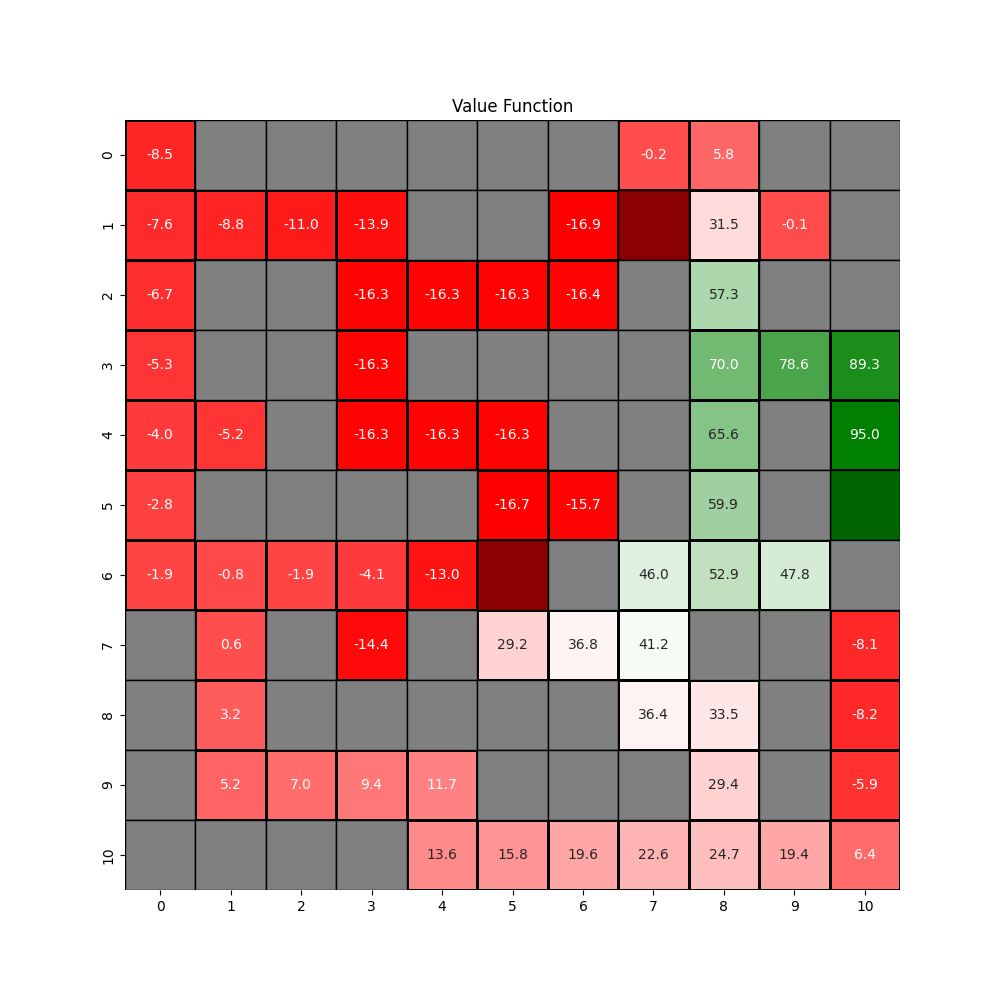
\includegraphics[width=\textwidth]{figures/value_q/default/value_function_alpha_0.1_gamma_0.95_epsilon_0.2_iteration_1000.png}
    \caption{Episode 1000.}
    \end{subfigure}\hfill
    \begin{subfigure}{0.3\textwidth}
        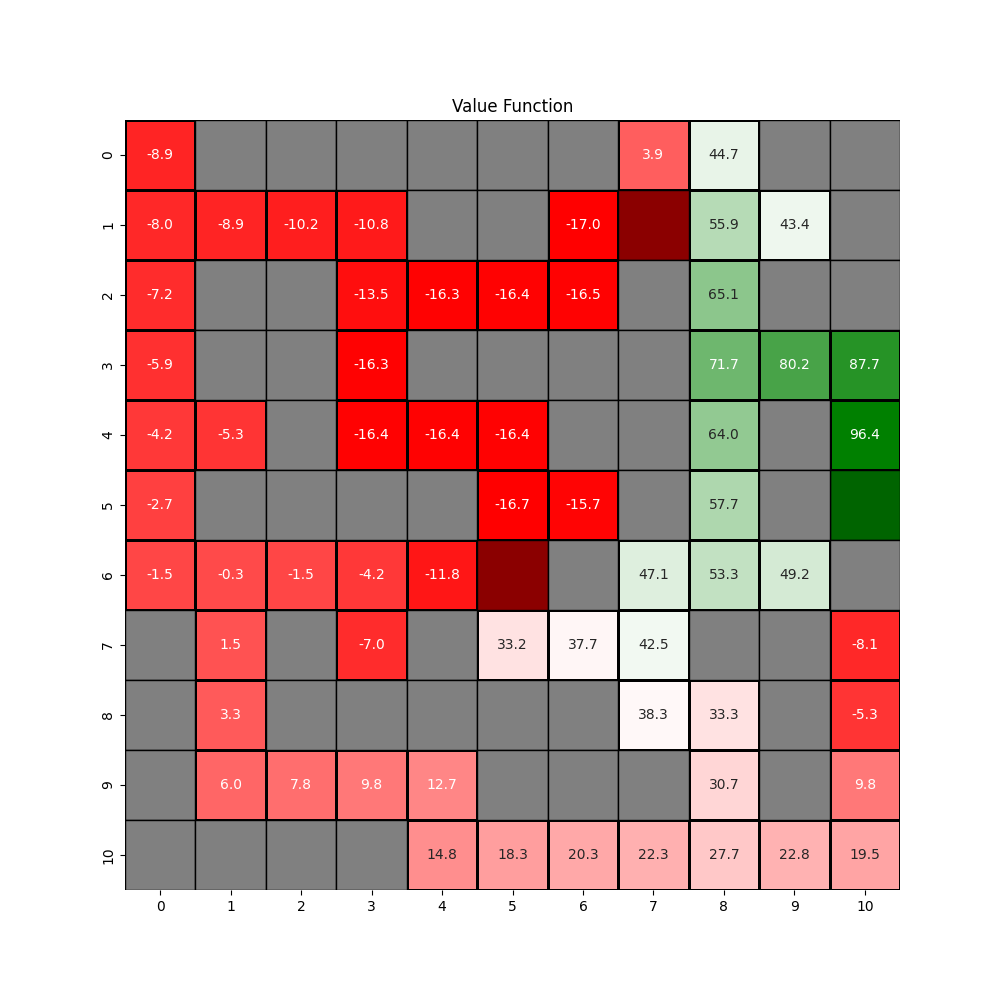
\includegraphics[width=\textwidth]{figures/value_q/default/value_function_alpha_0.1_gamma_0.95_epsilon_0.2_iteration_5000.png}
    \caption{Episode 5000}
    \end{subfigure}\hfill
    \begin{subfigure}{0.3\textwidth}
        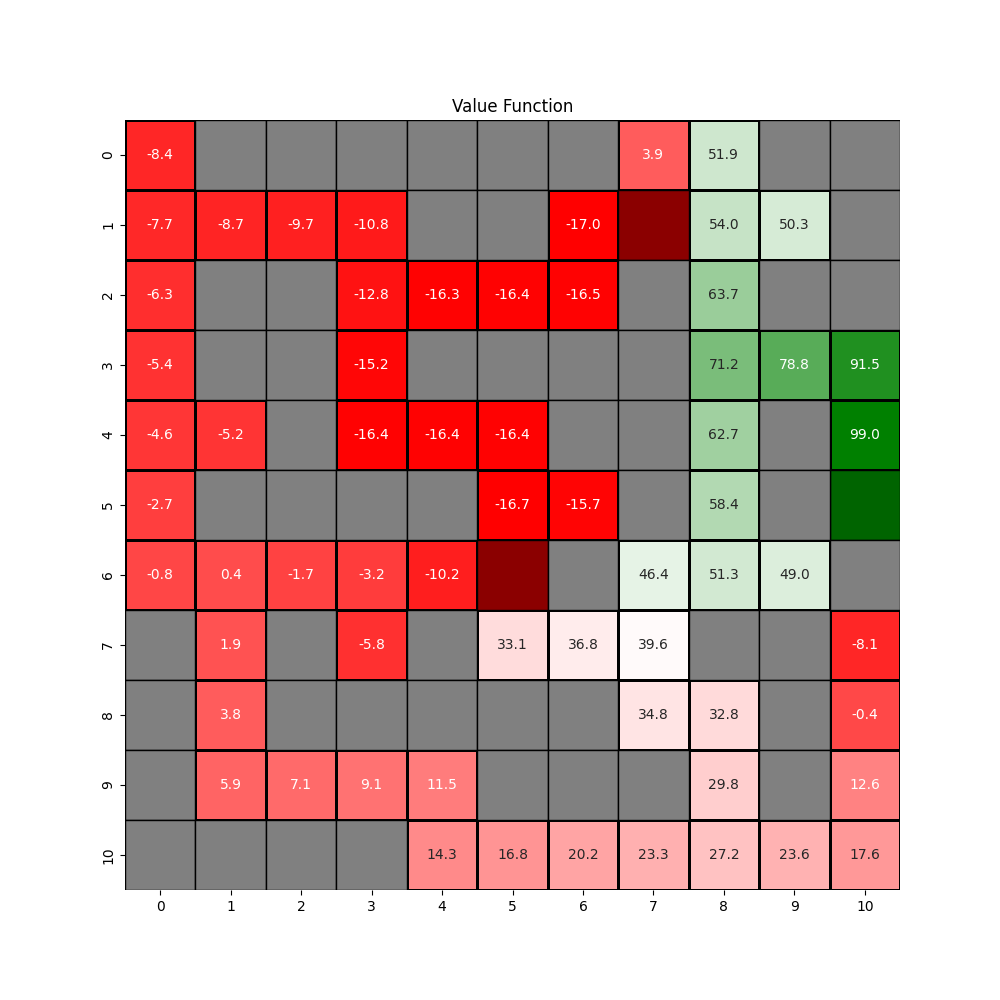
\includegraphics[width=\textwidth]{figures/value_q/default/value_function_alpha_0.1_gamma_0.95_epsilon_0.2_iteration_10000.png}
    \caption{Episode 10000}
    \end{subfigure}
    \caption{Evolution of value function throughout episodes.}
    \label{fig:default_q_learning_value}
\end{figure}


% convergence plots
\begin{figure}[H]
    \begin{subfigure}{0.5\textwidth}
        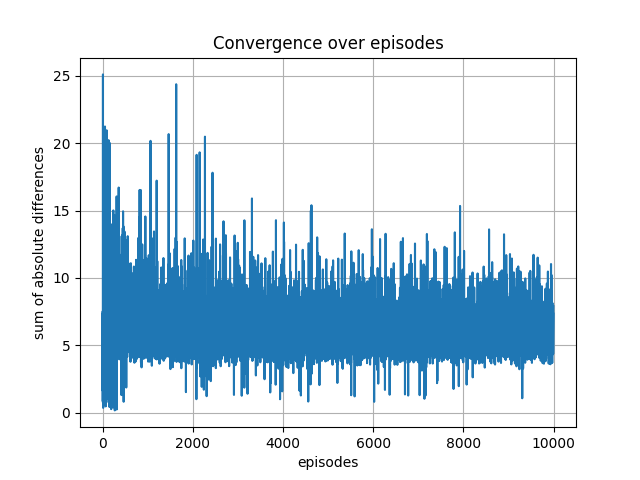
\includegraphics[width=\textwidth]{figures/convergence_q/default/convergence_Q_alpha_0.1_gamma_0.95_epislon_0.2.png}
    \caption{Converge raw.}
    \end{subfigure}\hfill
    \begin{subfigure}{0.5\textwidth}
        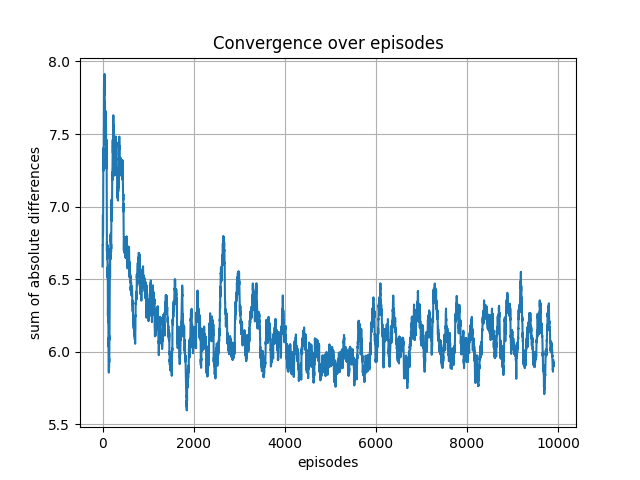
\includegraphics[width=\textwidth]{figures/convergence_q/default/convergence_Q_smoothed_alpha_0.1_gamma_0.95_epislon_0.2.png}
    \caption{Smoothed convergence.}
    \end{subfigure}
    \caption{Converge of value function.}
    \label{fig:default_q_learning_convergence}
\end{figure}




\subsection{Effect of Alpha in Temporal Difference Learning}
%parameters_alpha_sweep = [{"alpha": 0.001, "gamma": 0.95, "epsilon": 0.2, "episodes": 10000},
% {"alpha": 0.001, "gamma": 0.95, "epsilon": 0.2, "episodes": 10000},
% {"alpha": 0.1, "gamma": 0.95, "epsilon": 0.2, "episodes": 10000},
% {"alpha": 0.5, "gamma": 0.95, "epsilon": 0.2, "episodes": 10000},
% {"alpha": 1, "gamma": 0.95, "epsilon": 0.2, "episodes": 10000}]
Let us first provide the necessary output for each alpha parameter and then discuss the results at the end of this section.

Figure \ref{fig:alpha_0.001_td_learning_policy} provides the policy maps for the alpha parameter set to 0.001. Figure \ref{fig:alpha_0.001_td_learning_value} provides the value function plots for the alpha parameter set to 0.001. Figure \ref{fig:alpha_0.001_td_learning_convergence} provides the convergence plots for the alpha parameter set to 0.001.


% policy plots for alpha sweep of TD learning alpha = 0.001
\begin{figure}[H]
    \begin{subfigure}{0.3\textwidth}
        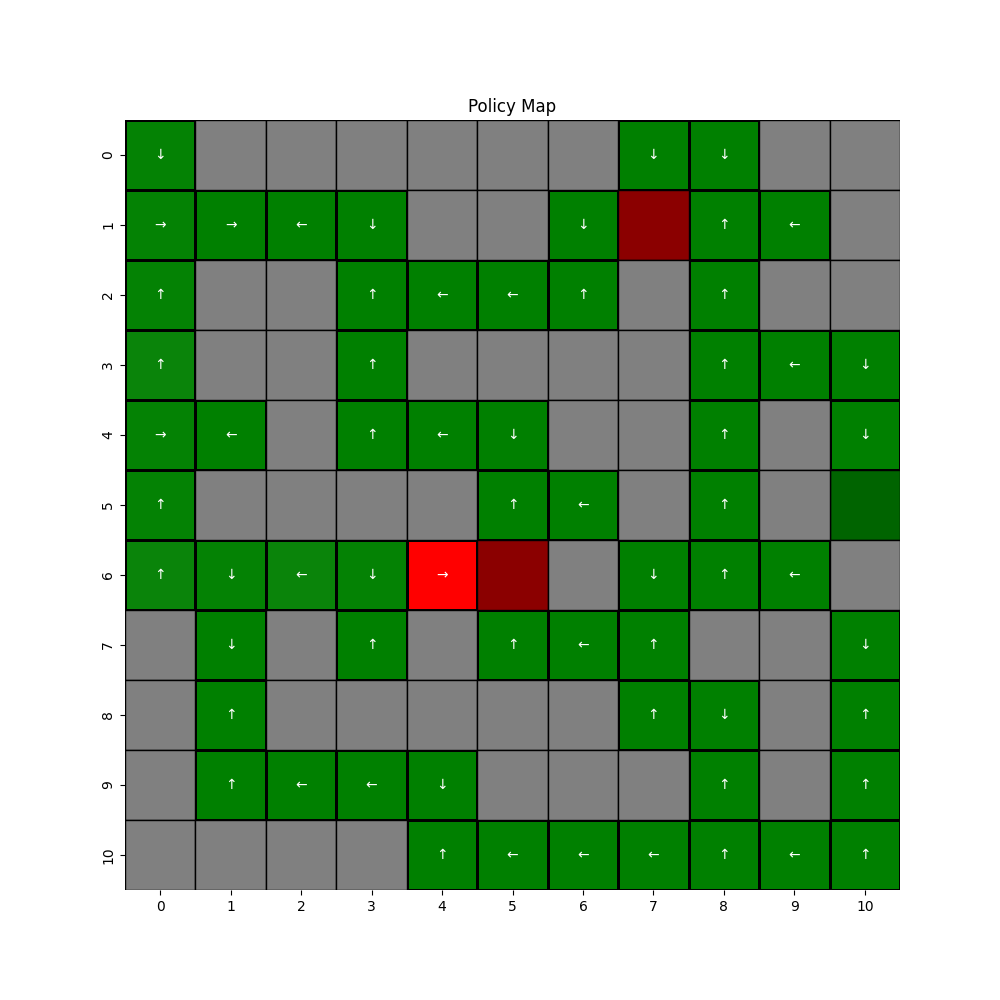
\includegraphics[width=\textwidth]{figures/policy_td/alpha_sweep/policy_alpha_0.001_gamma_0.95_epsilon_0.2_iteration_1.png}
    \caption{Episode 1.}
    \end{subfigure}\hfill
    \begin{subfigure}{0.3\textwidth}
        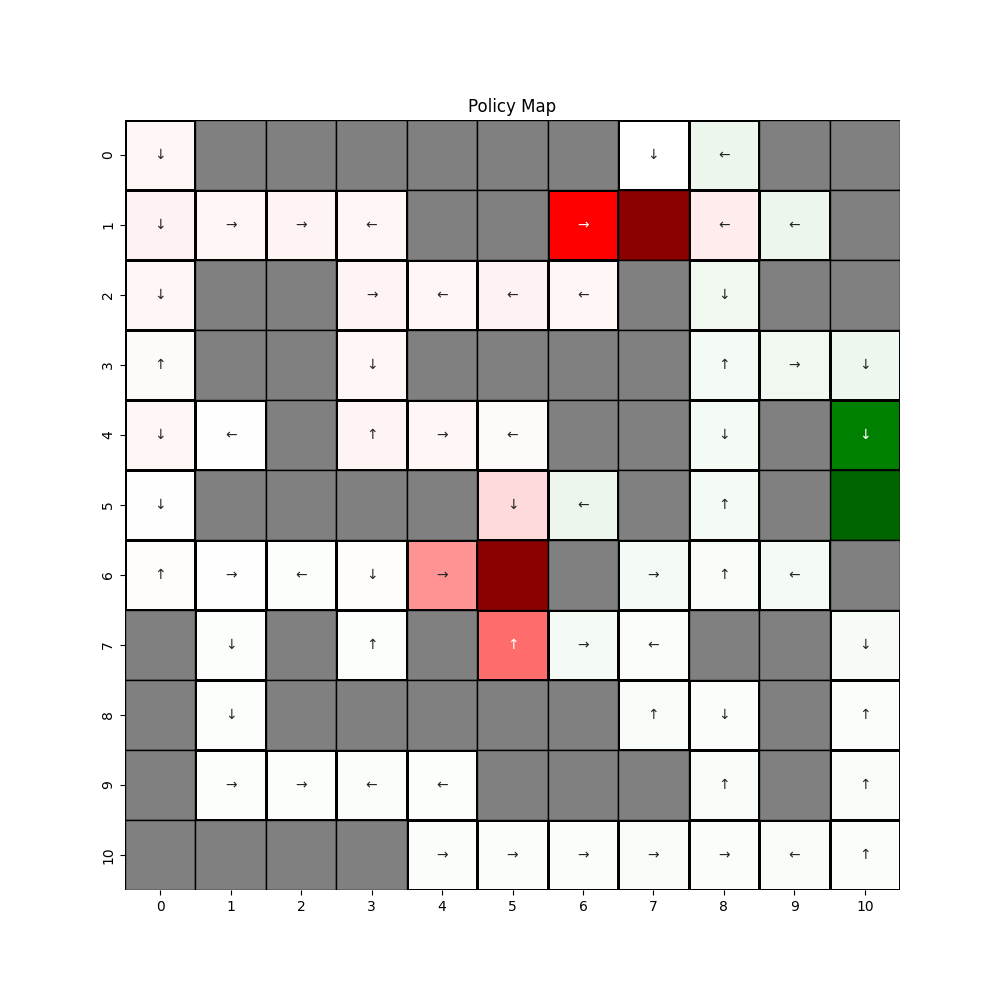
\includegraphics[width=\textwidth]{figures/policy_td/alpha_sweep/policy_alpha_0.001_gamma_0.95_epsilon_0.2_iteration_50.png}
    \caption{Episode 50}
    \end{subfigure}\hfill
    \begin{subfigure}{0.3\textwidth}
        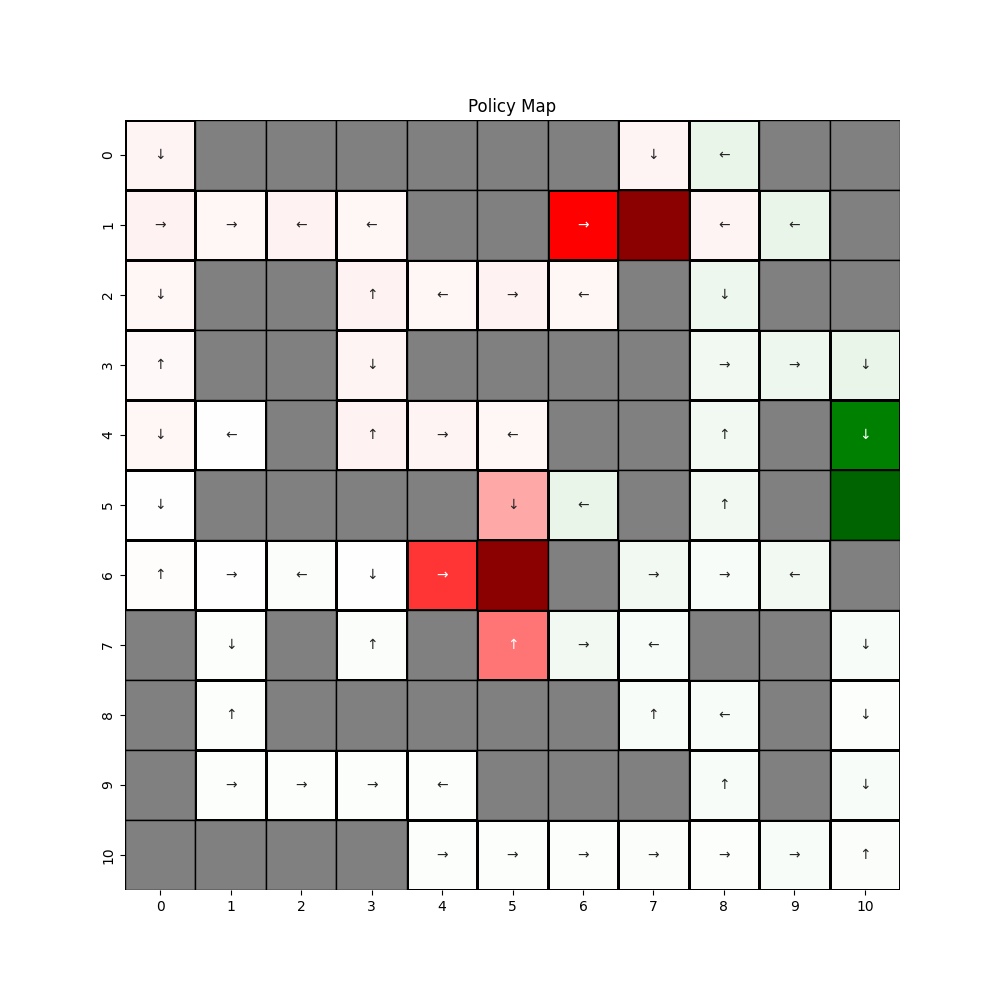
\includegraphics[width=\textwidth]{figures/policy_td/alpha_sweep/policy_alpha_0.001_gamma_0.95_epsilon_0.2_iteration_100.png}
    \caption{Episode 100}
    \end{subfigure}
    \begin{subfigure}{0.3\textwidth}
        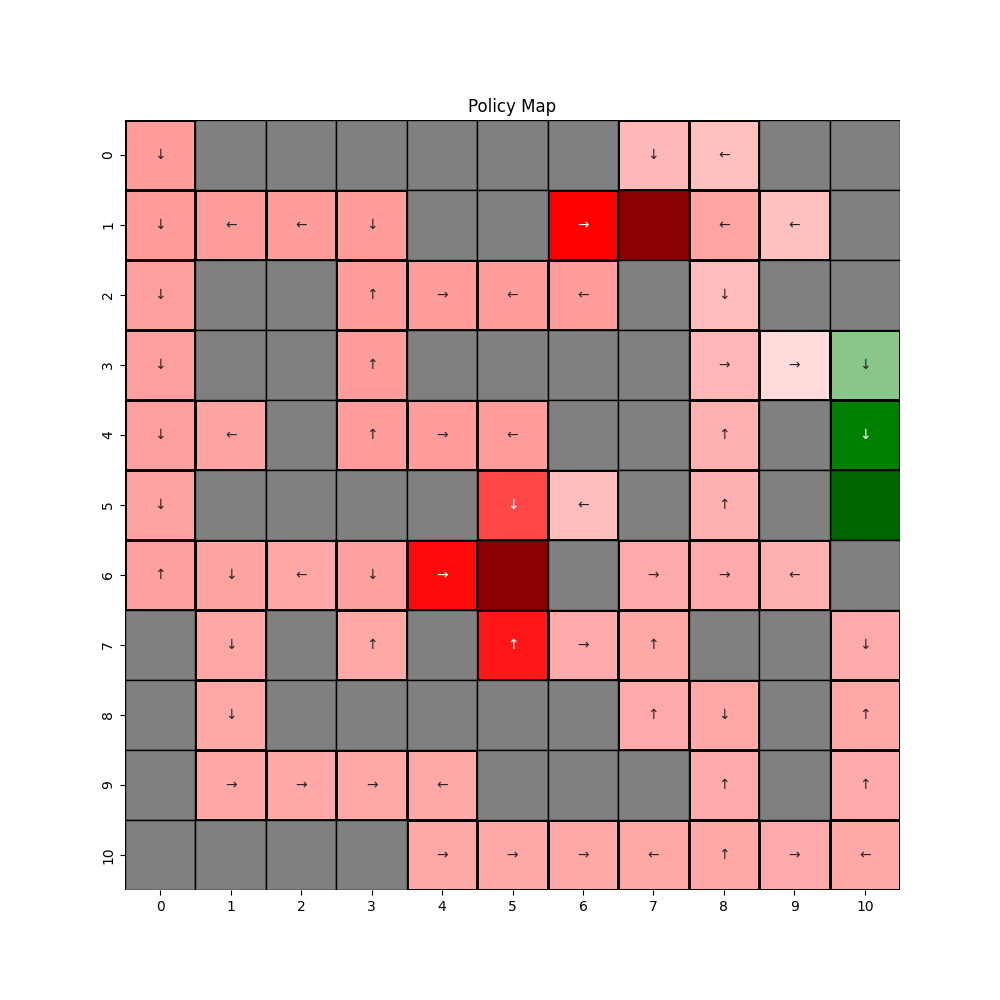
\includegraphics[width=\textwidth]{figures/policy_td/alpha_sweep/policy_alpha_0.001_gamma_0.95_epsilon_0.2_iteration_1000.png}
    \caption{Episode 1000.}
    \end{subfigure}\hfill
    \begin{subfigure}{0.3\textwidth}
        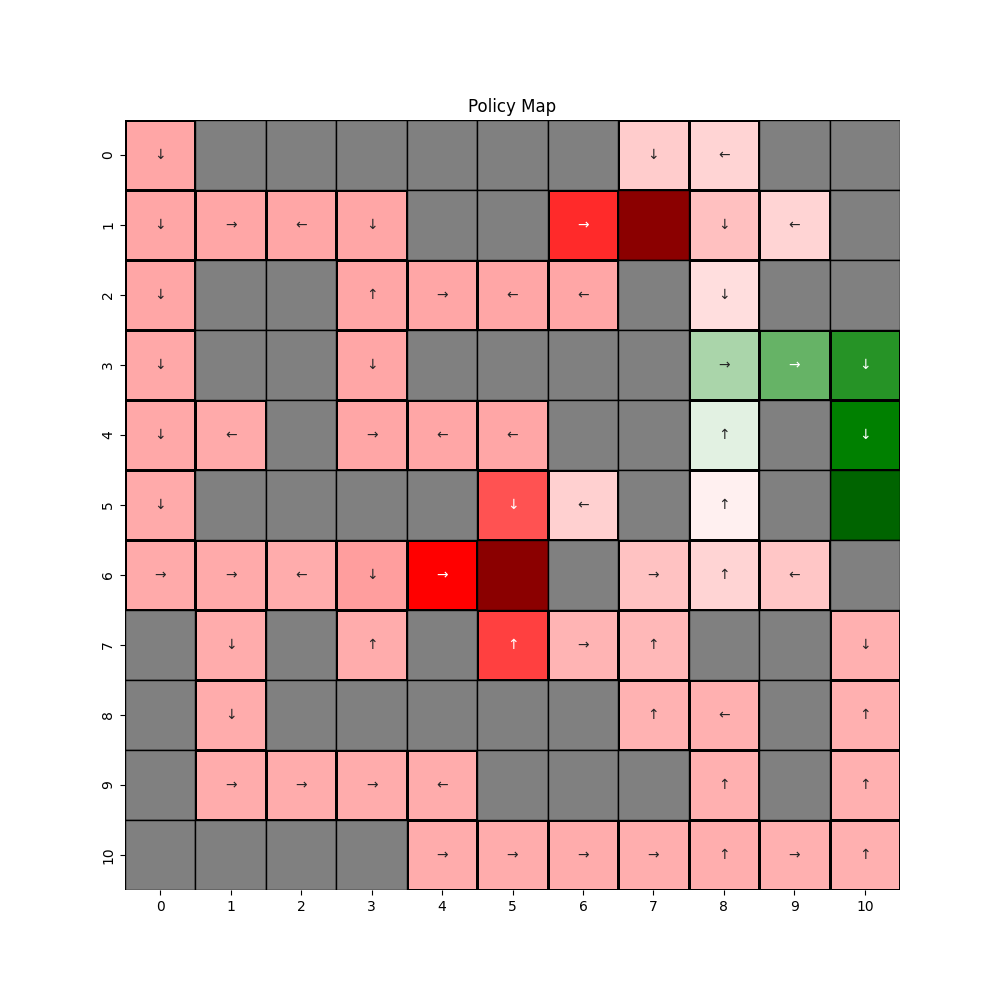
\includegraphics[width=\textwidth]{figures/policy_td/alpha_sweep/policy_alpha_0.001_gamma_0.95_epsilon_0.2_iteration_5000.png}
    \caption{Episode 5000}
    \end{subfigure}\hfill
    \begin{subfigure}{0.3\textwidth}
        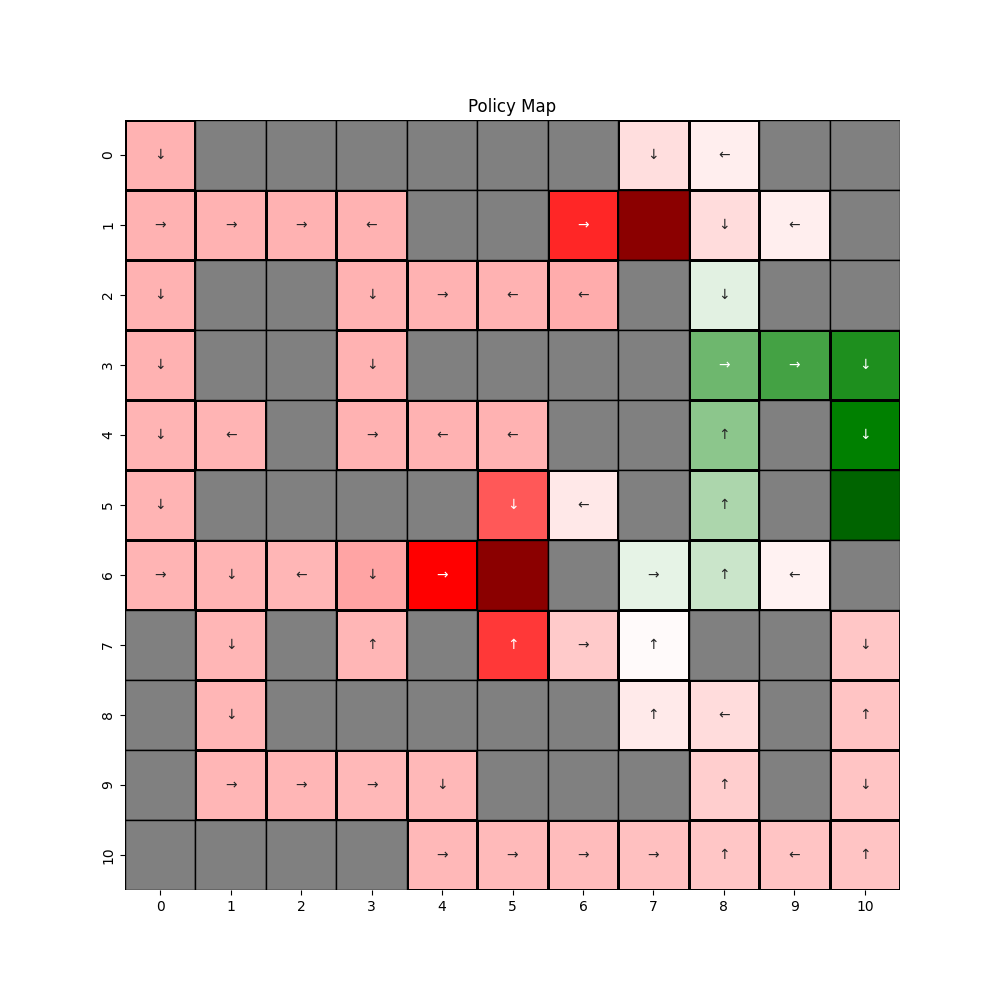
\includegraphics[width=\textwidth]{figures/policy_td/alpha_sweep/policy_alpha_0.001_gamma_0.95_epsilon_0.2_iteration_10000.png}
    \caption{Episode 10000}
    \end{subfigure}
    \caption{Evolution of policy maps throughout episodes.}
    \label{fig:alpha_0.001_td_learning_policy}
\end{figure}

% value plots for alpha sweep of TD learning alpha = 0.001
\begin{figure}[H]
    \begin{subfigure}{0.3\textwidth}
        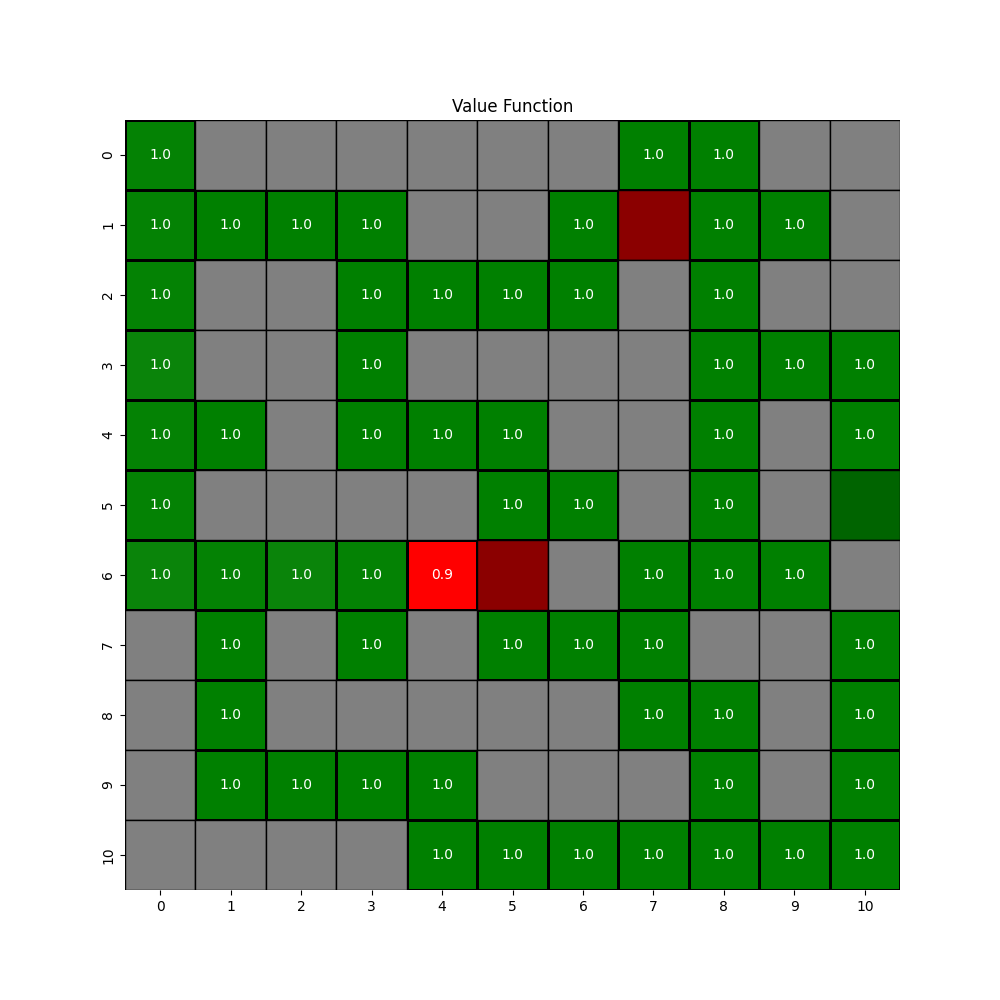
\includegraphics[width=\textwidth]{figures/value_td/alpha_sweep/value_function_alpha_0.001_gamma_0.95_epsilon_0.2_iteration_1.png}
    \caption{Episode 1.}
    \end{subfigure}\hfill
    \begin{subfigure}{0.3\textwidth}
        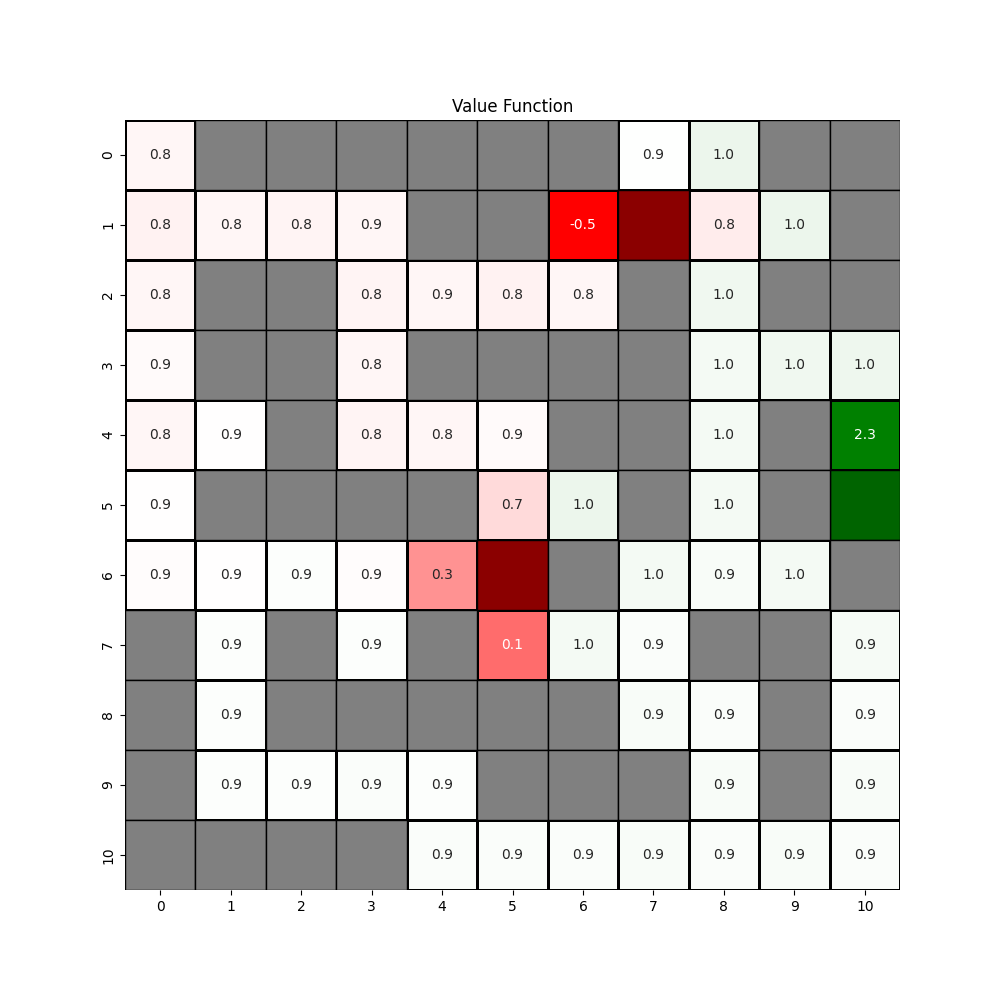
\includegraphics[width=\textwidth]{figures/value_td/alpha_sweep/value_function_alpha_0.001_gamma_0.95_epsilon_0.2_iteration_50.png}
    \caption{Episode 50}
    \end{subfigure}\hfill
    \begin{subfigure}{0.3\textwidth}
        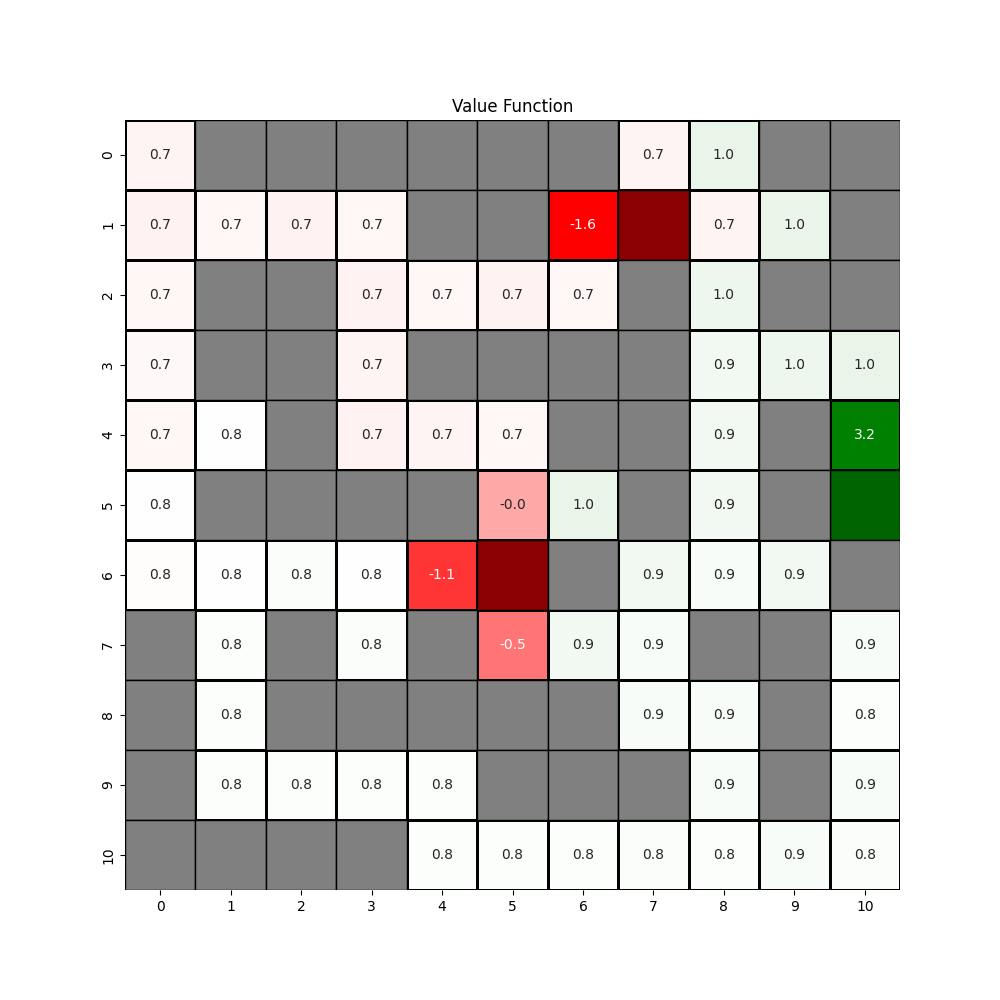
\includegraphics[width=\textwidth]{figures/value_td/alpha_sweep/value_function_alpha_0.001_gamma_0.95_epsilon_0.2_iteration_100.png}
    \caption{Episode 100}
    \end{subfigure}
    \begin{subfigure}{0.3\textwidth}
        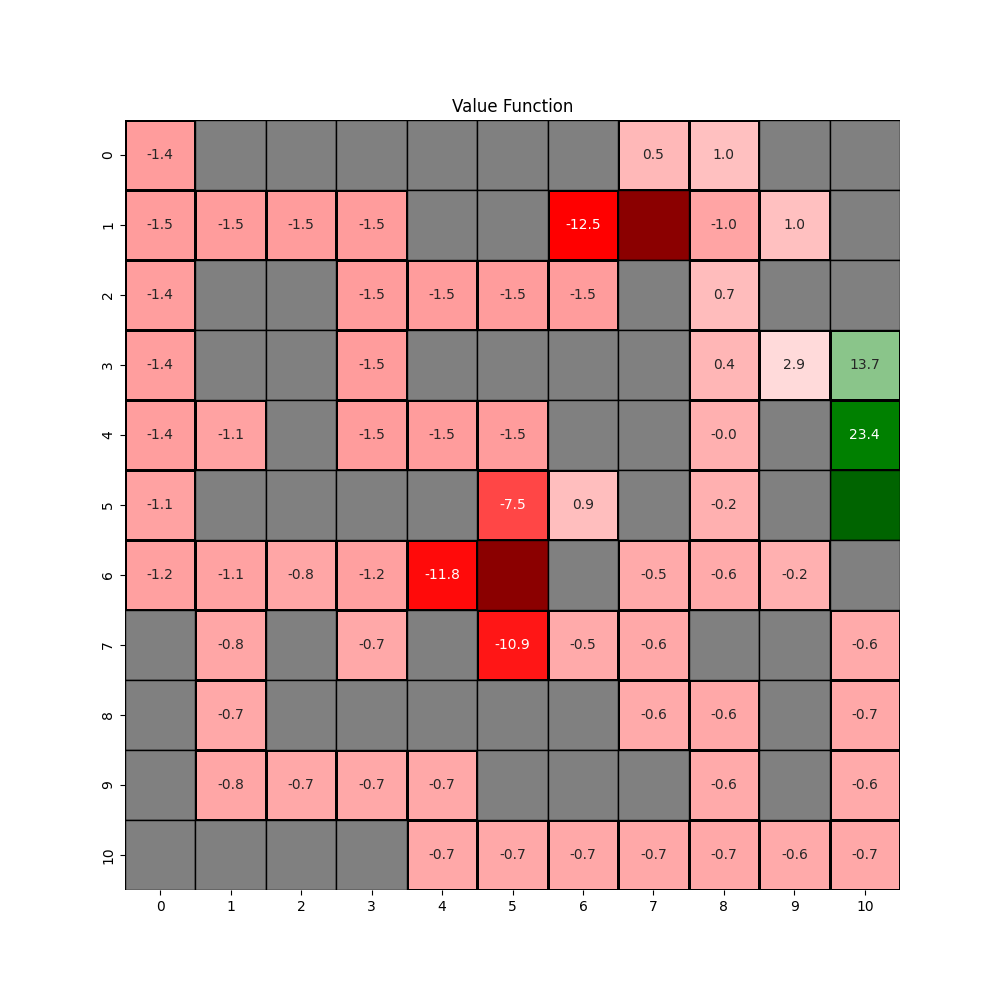
\includegraphics[width=\textwidth]{figures/value_td/alpha_sweep/value_function_alpha_0.001_gamma_0.95_epsilon_0.2_iteration_1000.png}
    \caption{Episode 1000.}
    \end{subfigure}\hfill
    \begin{subfigure}{0.3\textwidth}
        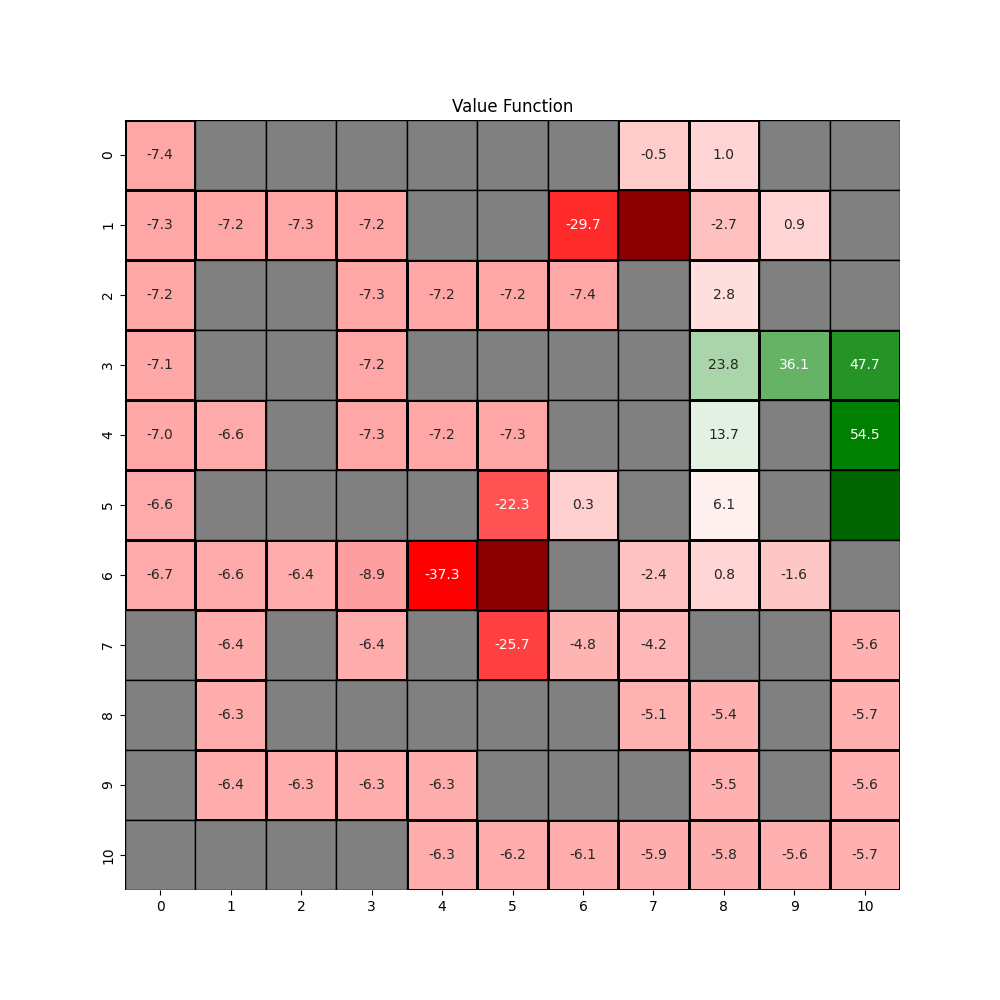
\includegraphics[width=\textwidth]{figures/value_td/alpha_sweep/value_function_alpha_0.001_gamma_0.95_epsilon_0.2_iteration_5000.png}
    \caption{Episode 5000}
    \end{subfigure}\hfill
    \begin{subfigure}{0.3\textwidth}
        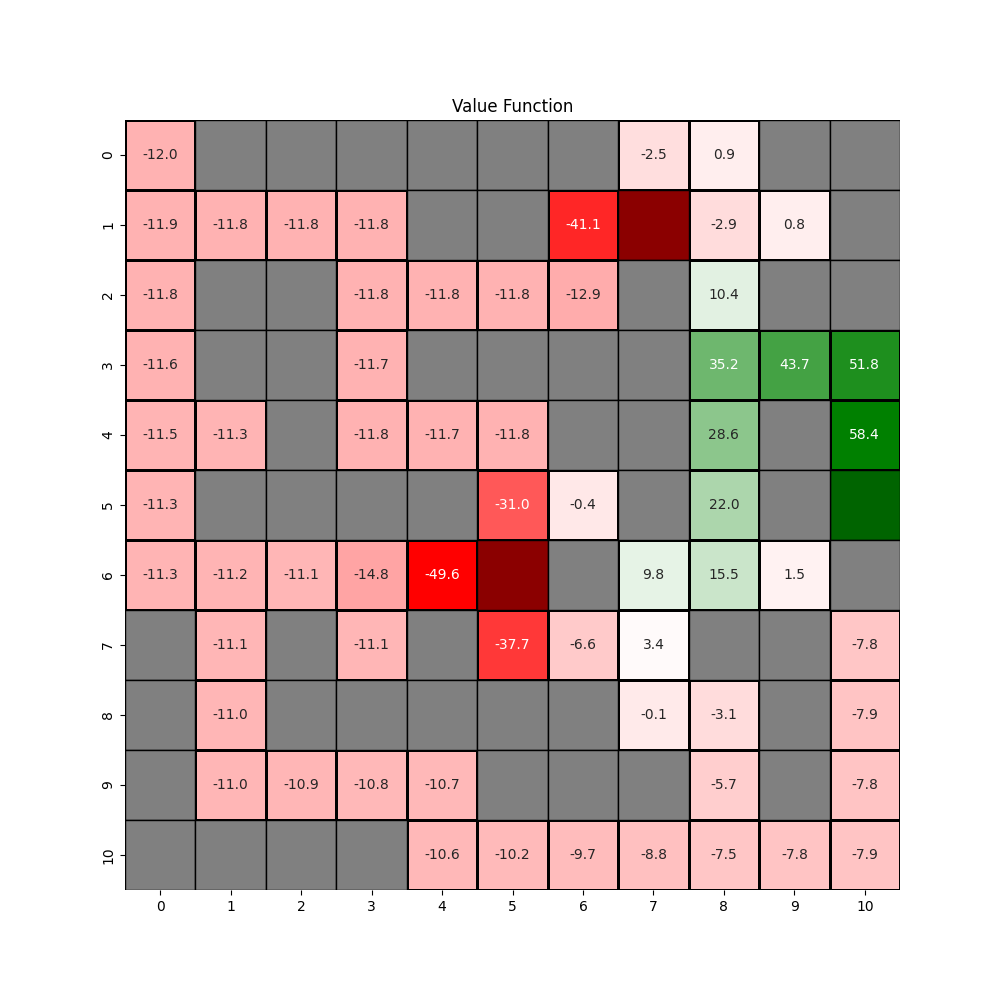
\includegraphics[width=\textwidth]{figures/value_td/alpha_sweep/value_function_alpha_0.001_gamma_0.95_epsilon_0.2_iteration_10000.png}
    \caption{Episode 10000}
    \end{subfigure}
    \caption{Evolution of value function throughout episodes.}
    \label{fig:alpha_0.001_td_learning_value}
\end{figure}

% convergence plots for alpha sweep of TD learning alpha = 0.001
\begin{figure}[H]
    \begin{subfigure}{0.5\textwidth}
        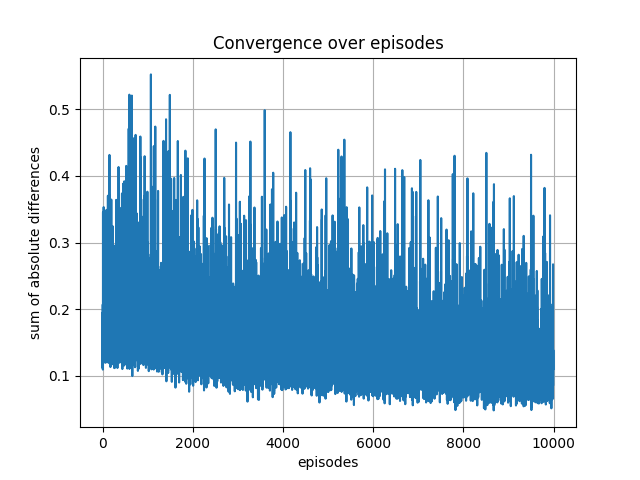
\includegraphics[width=\textwidth]{figures/convergence_td/alpha_sweep/convergence_TD_alpha_0.001_gamma_0.95_epislon_0.2.png}
    \caption{Converge raw.}
    \end{subfigure}\hfill
    \begin{subfigure}{0.5\textwidth}
        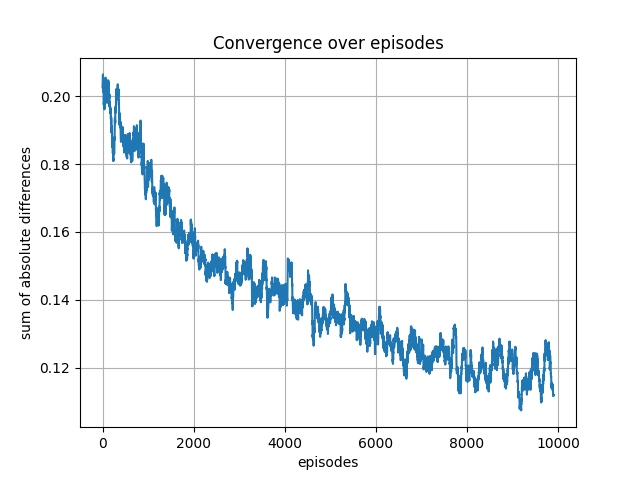
\includegraphics[width=\textwidth]{figures/convergence_td/alpha_sweep/convergence_TD_smoothed_alpha_0.001_gamma_0.95_epislon_0.2.png}
    \caption{Smoothed convergence.}
    \end{subfigure}
    \caption{Converge of value function.}
    \label{fig:alpha_0.001_td_learning_convergence}
\end{figure}

Figure \ref{fig:alpha_0.5_td_learning_policy} shows the policy maps for the alpha parameter set to 0.5. Figure \ref{fig:alpha_0.5_td_learning_value} illustrates the value function plots for the alpha parameter set to 0.5. Figure \ref{fig:alpha_0.5_td_learning_convergence} provides the convergence plots for the alpha parameter set to 0.5.

% policy plots for alpha sweep of TD learning alpha = 0.5
\begin{figure}[H]
    \begin{subfigure}{0.3\textwidth}
        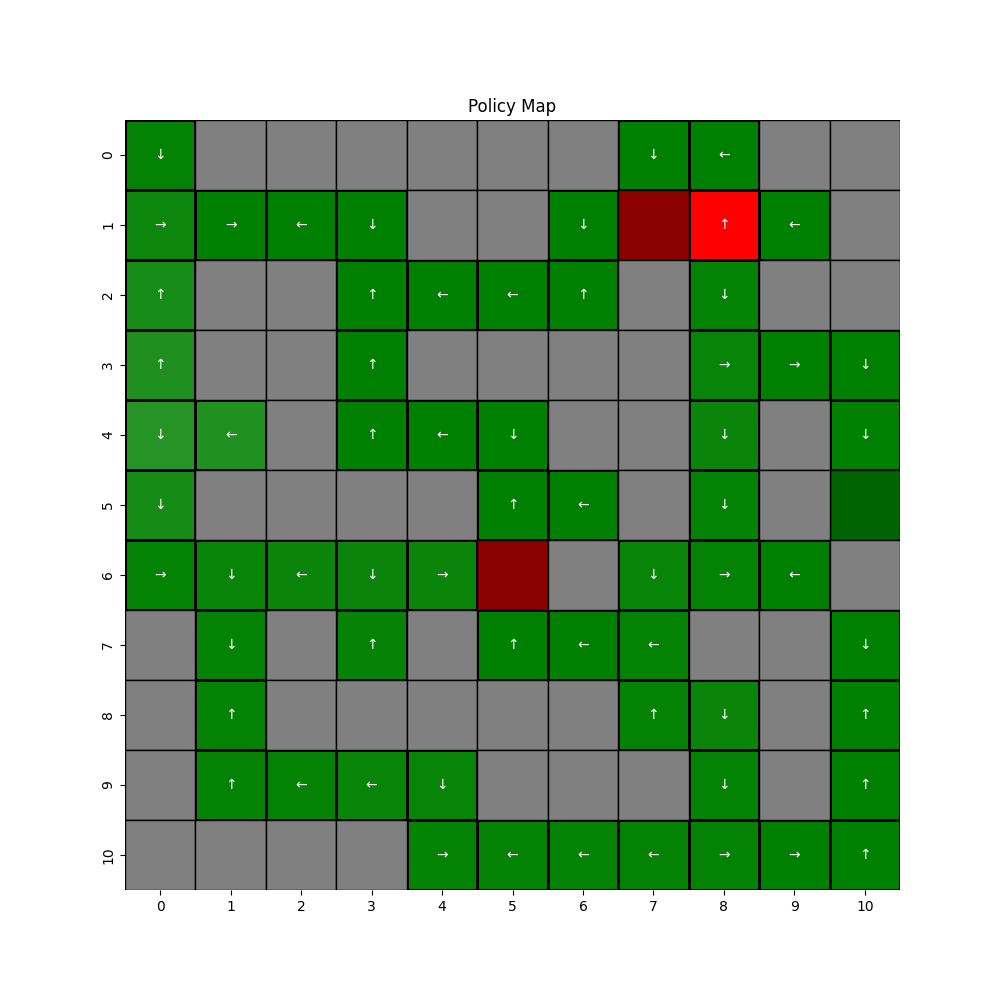
\includegraphics[width=\textwidth]{figures/policy_td/alpha_sweep/policy_alpha_0.5_gamma_0.95_epsilon_0.2_iteration_1.png}
    \caption{Episode 1.}
    \end{subfigure}\hfill
    \begin{subfigure}{0.3\textwidth}
        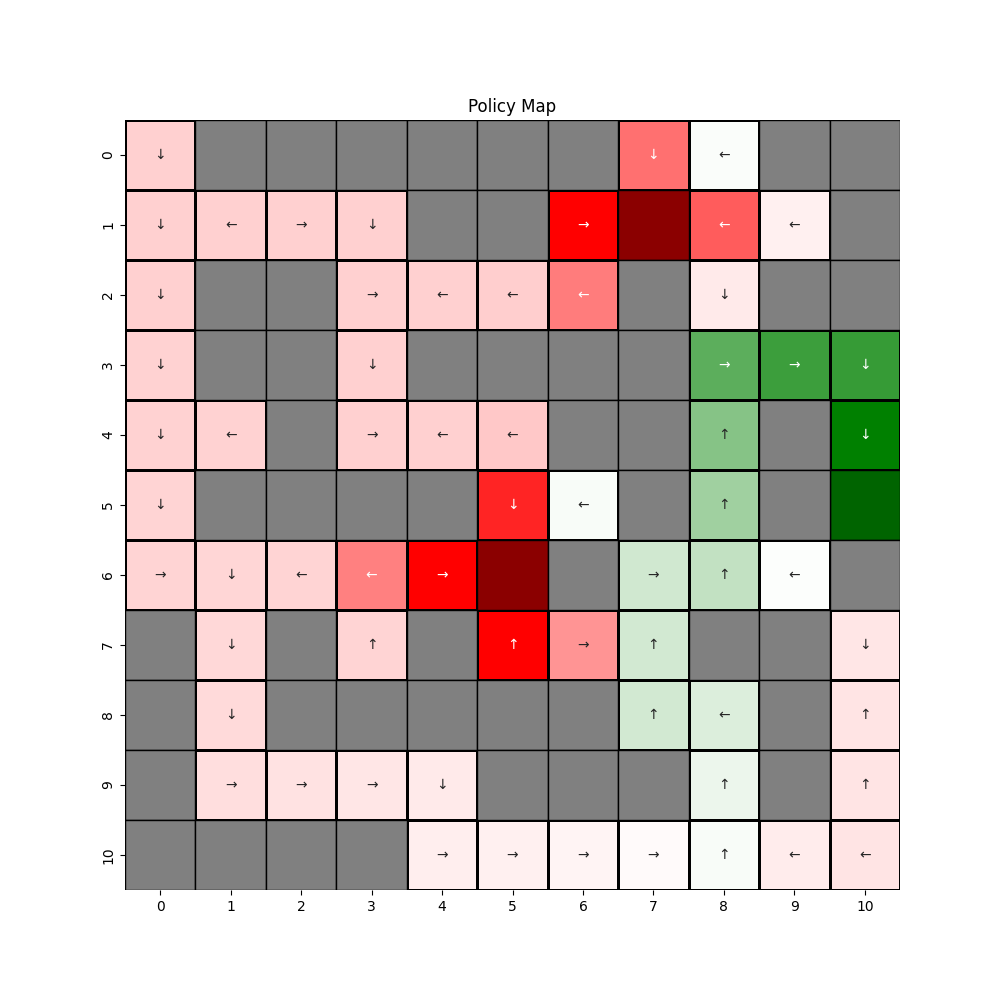
\includegraphics[width=\textwidth]{figures/policy_td/alpha_sweep/policy_alpha_0.5_gamma_0.95_epsilon_0.2_iteration_50.png}
    \caption{Episode 50}
    \end{subfigure}\hfill
    \begin{subfigure}{0.3\textwidth}
        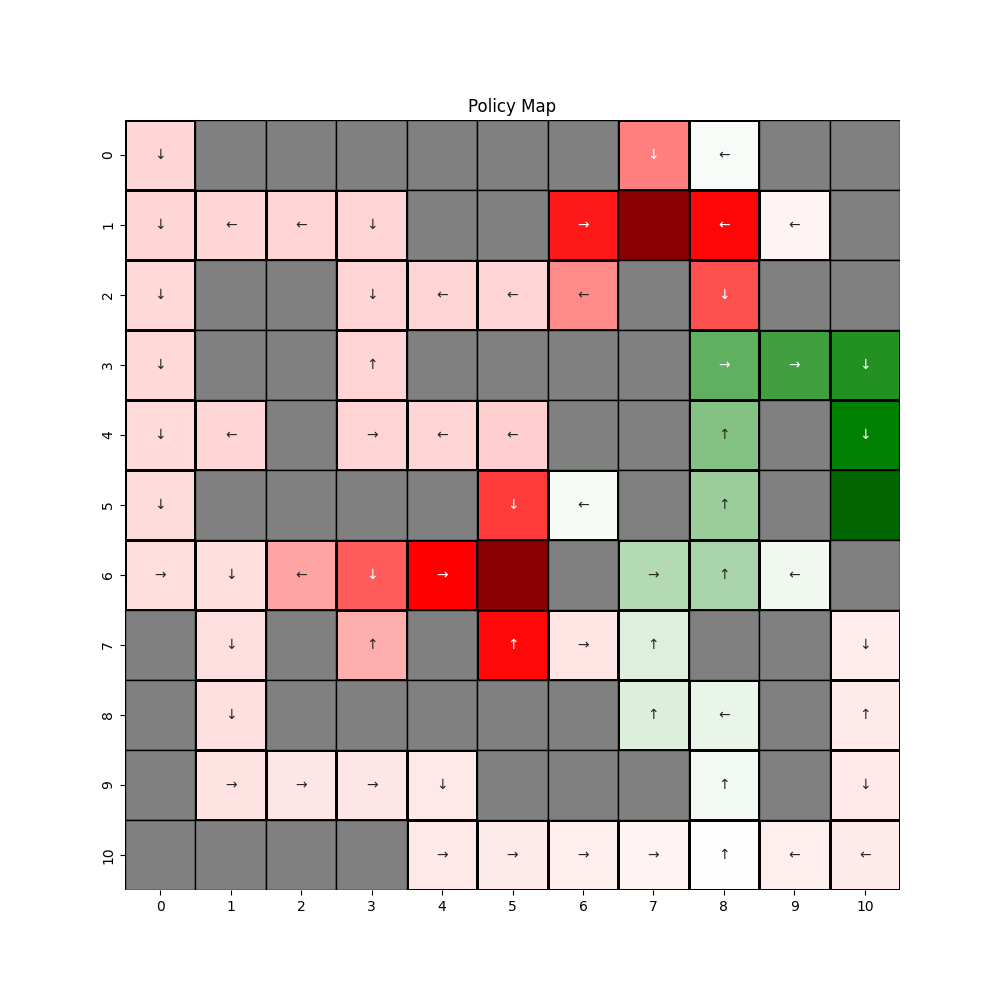
\includegraphics[width=\textwidth]{figures/policy_td/alpha_sweep/policy_alpha_0.5_gamma_0.95_epsilon_0.2_iteration_100.png}
    \caption{Episode 100}
    \end{subfigure}
    \begin{subfigure}{0.3\textwidth}
        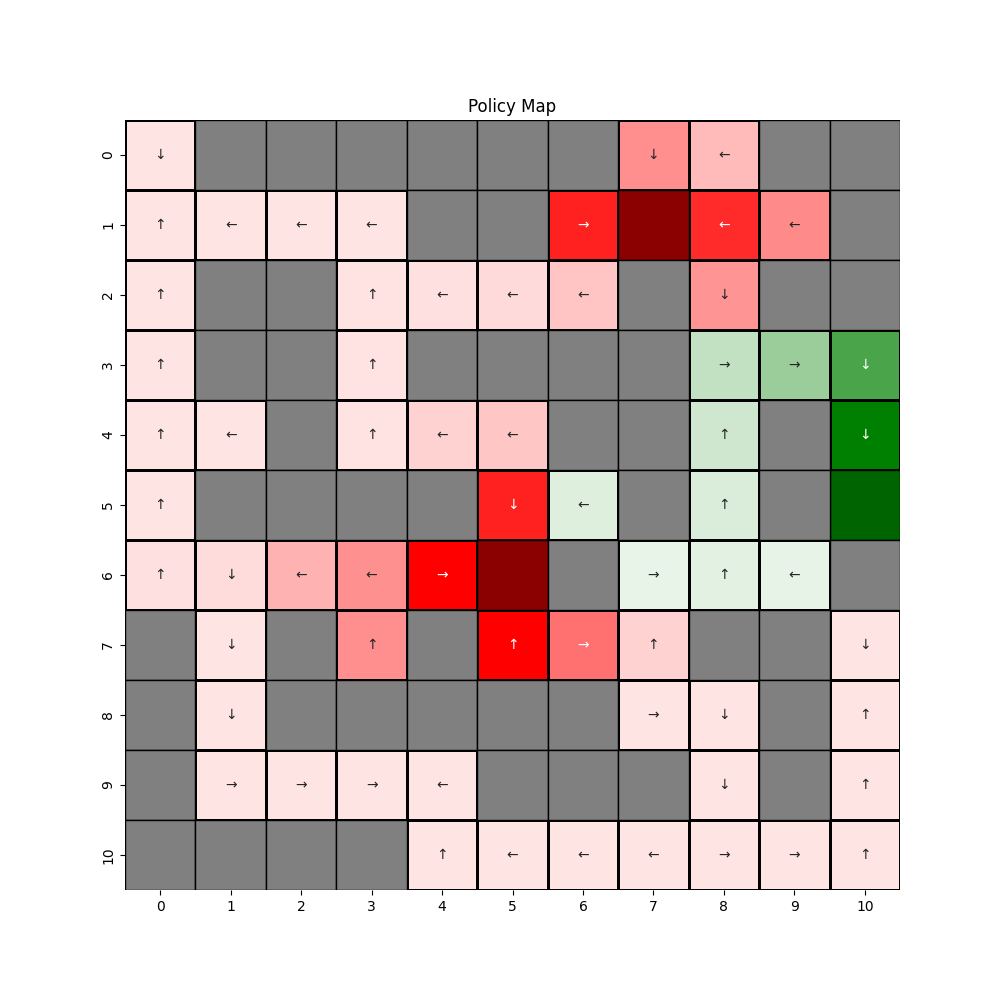
\includegraphics[width=\textwidth]{figures/policy_td/alpha_sweep/policy_alpha_0.5_gamma_0.95_epsilon_0.2_iteration_1000.png}
    \caption{Episode 1000.}
    \end{subfigure}\hfill
    \begin{subfigure}{0.3\textwidth}
        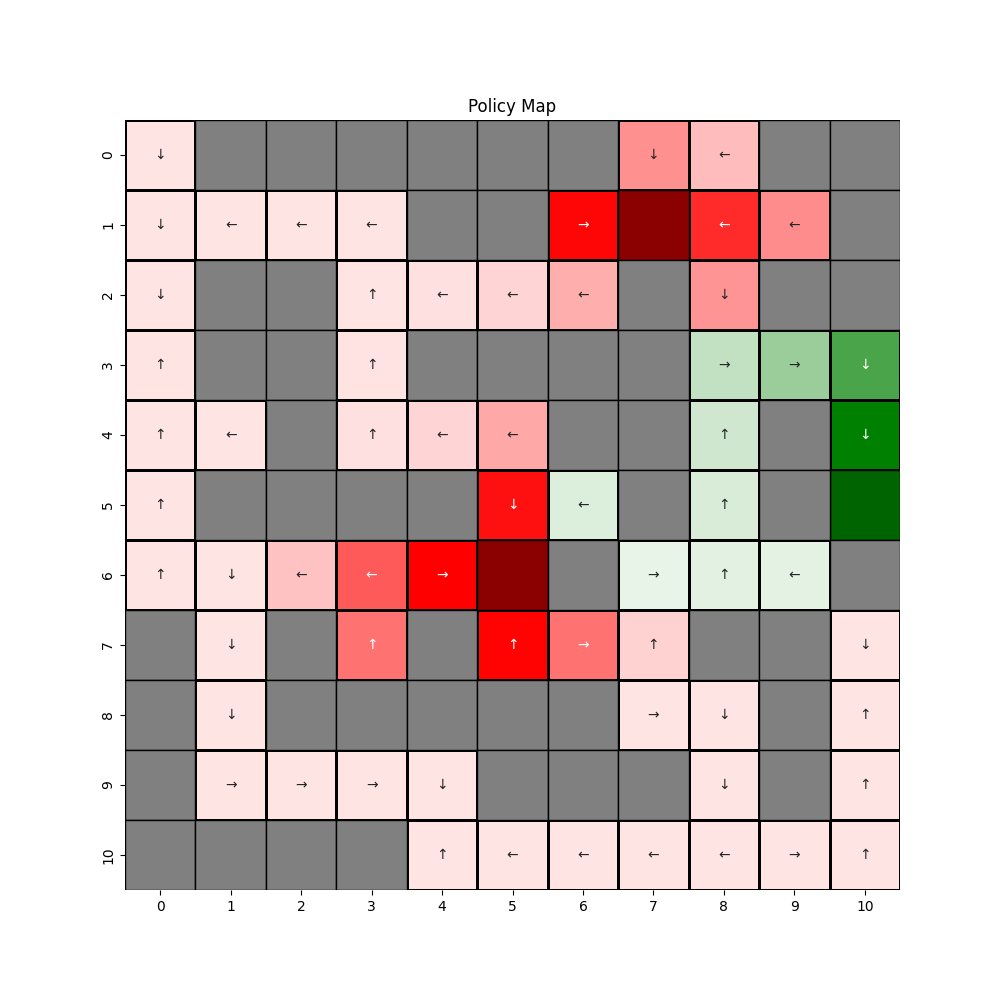
\includegraphics[width=\textwidth]{figures/policy_td/alpha_sweep/policy_alpha_0.5_gamma_0.95_epsilon_0.2_iteration_5000.png}
    \caption{Episode 5000}
    \end{subfigure}\hfill
    \begin{subfigure}{0.3\textwidth}
        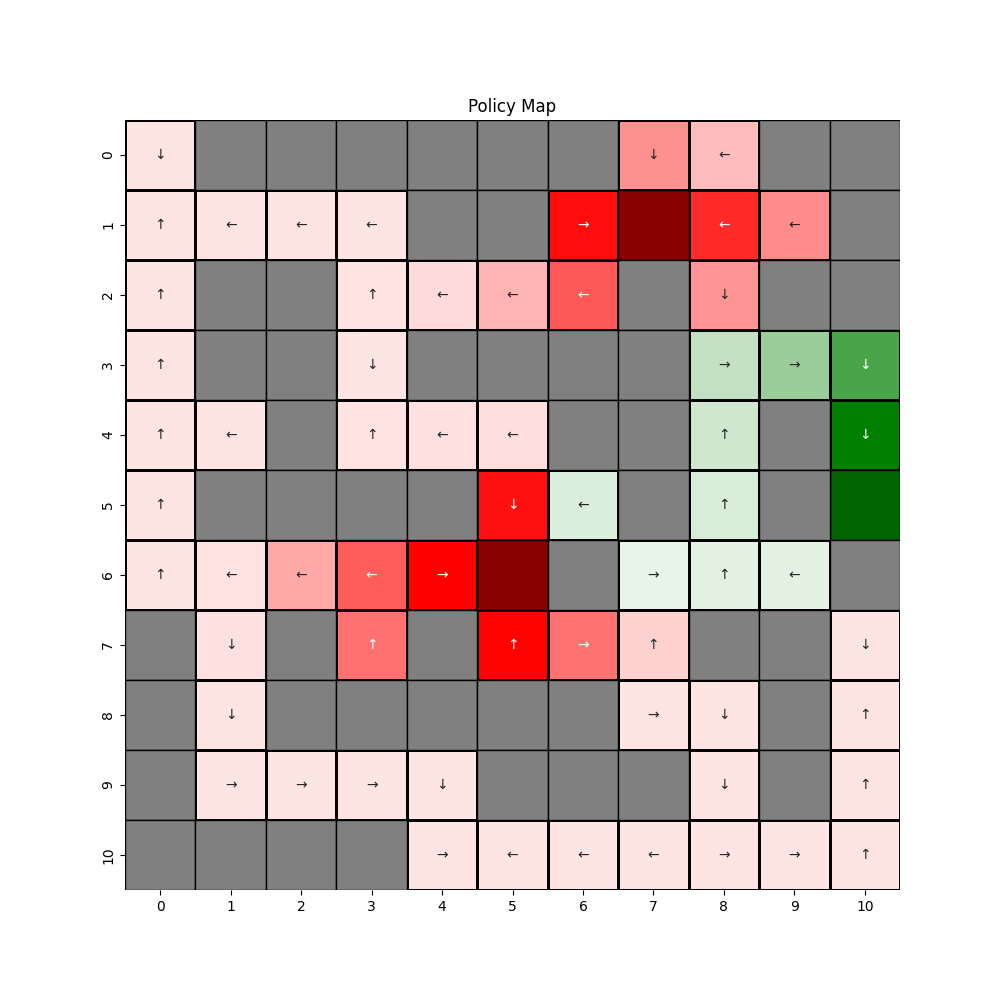
\includegraphics[width=\textwidth]{figures/policy_td/alpha_sweep/policy_alpha_0.5_gamma_0.95_epsilon_0.2_iteration_10000.png}
    \caption{Episode 10000}
    \end{subfigure}
    \caption{Evolution of policy maps throughout episodes.}
    \label{fig:alpha_0.5_td_learning_policy}
\end{figure}

% value plots for alpha sweep of TD learning alpha = 0.5
\begin{figure}[H]
    \begin{subfigure}{0.3\textwidth}
        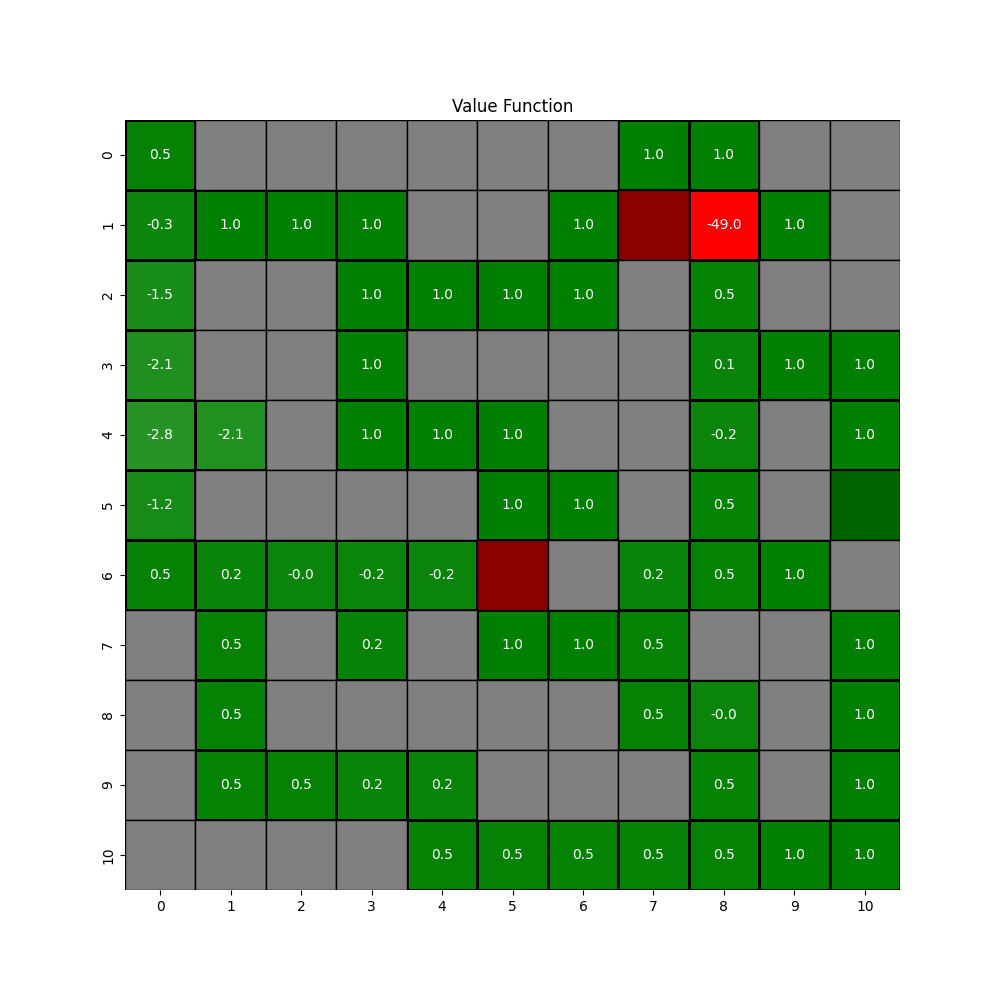
\includegraphics[width=\textwidth]{figures/value_td/alpha_sweep/value_function_alpha_0.5_gamma_0.95_epsilon_0.2_iteration_1.png}
    \caption{Episode 1.}
    \end{subfigure}\hfill
    \begin{subfigure}{0.3\textwidth}
        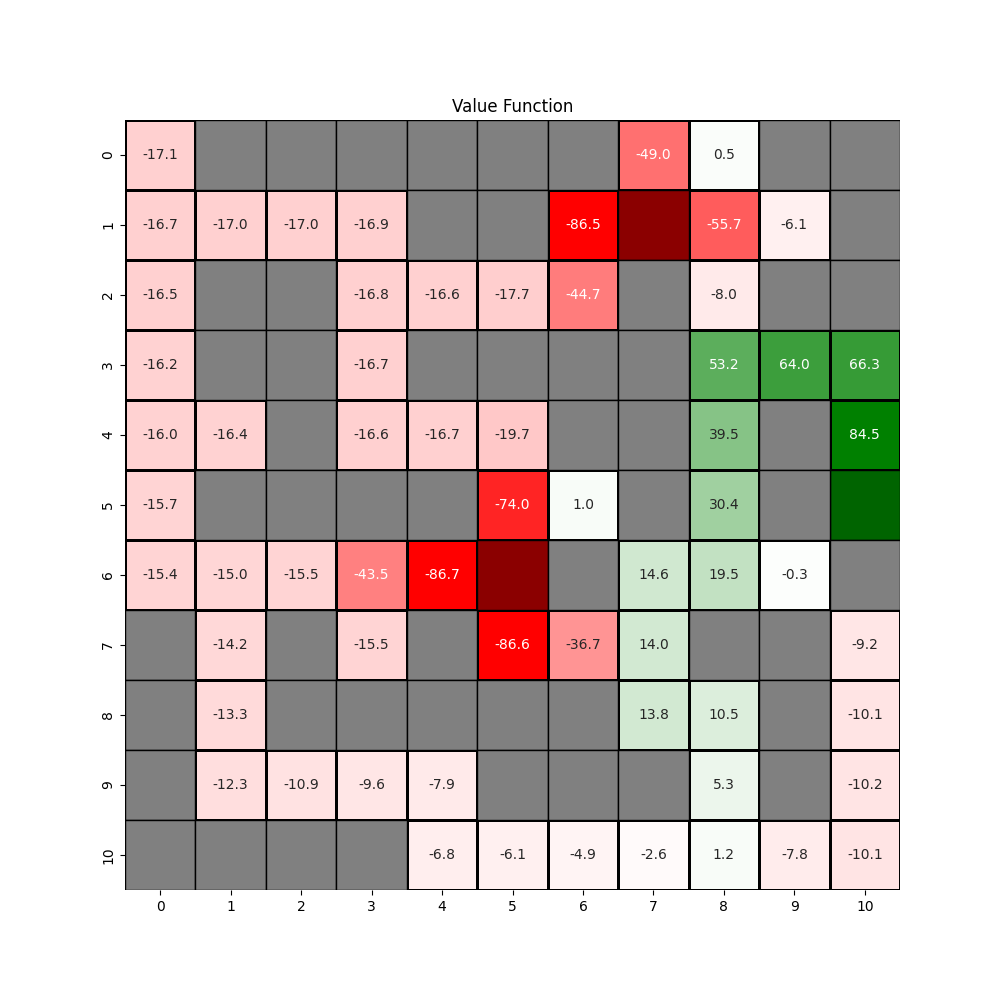
\includegraphics[width=\textwidth]{figures/value_td/alpha_sweep/value_function_alpha_0.5_gamma_0.95_epsilon_0.2_iteration_50.png}
    \caption{Episode 50}
    \end{subfigure}\hfill
    \begin{subfigure}{0.3\textwidth}
        \includegraphics[width=\textwidth]{figures/value_td/alpha_sweep/value_function_alpha_0.5_gamma_0.95_epsilon_0.2_iteration_100.png}
    \caption{Episode 100}
    \end{subfigure}
    \begin{subfigure}{0.3\textwidth}
        \includegraphics[width=\textwidth]{figures/value_td/alpha_sweep/value_function_alpha_0.5_gamma_0.95_epsilon_0.2_iteration_1000.png}
    \caption{Episode 1000.}
    \end{subfigure}\hfill
    \begin{subfigure}{0.3\textwidth}
        \includegraphics[width=\textwidth]{figures/value_td/alpha_sweep/value_function_alpha_0.5_gamma_0.95_epsilon_0.2_iteration_5000.png}
    \caption{Episode 5000}
    \end{subfigure}\hfill
    \begin{subfigure}{0.3\textwidth}
        \includegraphics[width=\textwidth]{figures/value_td/alpha_sweep/value_function_alpha_0.5_gamma_0.95_epsilon_0.2_iteration_10000.png}
    \caption{Episode 10000}
    \end{subfigure}
    \caption{Evolution of value function throughout episodes.}
    \label{fig:alpha_0.5_td_learning_value}
\end{figure}

% convergence plots for alpha sweep of TD learning alpha = 0.5
\begin{figure}[H]
    \begin{subfigure}{0.5\textwidth}
        \includegraphics[width=\textwidth]{figures/convergence_td/alpha_sweep/convergence_TD_alpha_0.5_gamma_0.95_epislon_0.2.png}
    \caption{Converge raw.}
    \end{subfigure}\hfill
    \begin{subfigure}{0.5\textwidth}
        \includegraphics[width=\textwidth]{figures/convergence_td/alpha_sweep/convergence_TD_smoothed_alpha_0.5_gamma_0.95_epislon_0.2.png}
    \caption{Smoothed convergence.}
    \end{subfigure}
    \caption{Converge of value function.}
    \label{fig:alpha_0.5_td_learning_convergence}
\end{figure}

Lastly, Figure \ref{fig:alpha_1_td_learning_policy} shows the policy maps for the alpha parameter set to 1. Figure \ref{fig:alpha_1_td_learning_value} illustrates the value function plots for the alpha parameter set to 1. Figure \ref{fig:alpha_1_td_learning_convergence} provides the convergence plots for the alpha parameter set to 1.

% policy plots for alpha sweep of TD learning alpha = 1
\begin{figure}[H]
    \begin{subfigure}{0.3\textwidth}
        \includegraphics[width=\textwidth]{figures/policy_td/alpha_sweep/policy_alpha_1_gamma_0.95_epsilon_0.2_iteration_1.png}
    \caption{Episode 1.}
    \end{subfigure}\hfill
    \begin{subfigure}{0.3\textwidth}
        \includegraphics[width=\textwidth]{figures/policy_td/alpha_sweep/policy_alpha_1_gamma_0.95_epsilon_0.2_iteration_50.png}
    \caption{Episode 50}
    \end{subfigure}\hfill
    \begin{subfigure}{0.3\textwidth}
        \includegraphics[width=\textwidth]{figures/policy_td/alpha_sweep/policy_alpha_1_gamma_0.95_epsilon_0.2_iteration_100.png}
    \caption{Episode 100}
    \end{subfigure}
    \begin{subfigure}{0.3\textwidth}
        \includegraphics[width=\textwidth]{figures/policy_td/alpha_sweep/policy_alpha_1_gamma_0.95_epsilon_0.2_iteration_1000.png}
    \caption{Episode 1000.}
    \end{subfigure}\hfill
    \begin{subfigure}{0.3\textwidth}
        \includegraphics[width=\textwidth]{figures/policy_td/alpha_sweep/policy_alpha_1_gamma_0.95_epsilon_0.2_iteration_5000.png}
    \caption{Episode 5000}
    \end{subfigure}\hfill
    \begin{subfigure}{0.3\textwidth}
        \includegraphics[width=\textwidth]{figures/policy_td/alpha_sweep/policy_alpha_1_gamma_0.95_epsilon_0.2_iteration_10000.png}
    \caption{Episode 10000}
    \end{subfigure}
    \caption{Evolution of policy maps throughout episodes.}
    \label{fig:alpha_1_td_learning_policy}
\end{figure}

% value plots for alpha sweep of TD learning alpha = 1
\begin{figure}[H]
    \begin{subfigure}{0.3\textwidth}
        \includegraphics[width=\textwidth]{figures/value_td/alpha_sweep/value_function_alpha_1_gamma_0.95_epsilon_0.2_iteration_1.png}
    \caption{Episode 1.}
    \end{subfigure}\hfill
    \begin{subfigure}{0.3\textwidth}
        \includegraphics[width=\textwidth]{figures/value_td/alpha_sweep/value_function_alpha_1_gamma_0.95_epsilon_0.2_iteration_50.png}
    \caption{Episode 50}
    \end{subfigure}\hfill
    \begin{subfigure}{0.3\textwidth}
        \includegraphics[width=\textwidth]{figures/value_td/alpha_sweep/value_function_alpha_1_gamma_0.95_epsilon_0.2_iteration_100.png}
    \caption{Episode 100}
    \end{subfigure}
    \begin{subfigure}{0.3\textwidth}
        \includegraphics[width=\textwidth]{figures/value_td/alpha_sweep/value_function_alpha_1_gamma_0.95_epsilon_0.2_iteration_1000.png}
    \caption{Episode 1000.}
    \end{subfigure}\hfill
    \begin{subfigure}{0.3\textwidth}
        \includegraphics[width=\textwidth]{figures/value_td/alpha_sweep/value_function_alpha_1_gamma_0.95_epsilon_0.2_iteration_5000.png}
    \caption{Episode 5000}
    \end{subfigure}\hfill
    \begin{subfigure}{0.3\textwidth}
        \includegraphics[width=\textwidth]{figures/value_td/alpha_sweep/value_function_alpha_1_gamma_0.95_epsilon_0.2_iteration_10000.png}
    \caption{Episode 10000}
    \end{subfigure}
    \caption{Evolution of value function throughout episodes.}
    \label{fig:alpha_1_td_learning_value}
\end{figure}

% convergence plots for alpha sweep of TD learning alpha = 1
\begin{figure}[H]
    \begin{subfigure}{0.5\textwidth}
        \includegraphics[width=\textwidth]{figures/convergence_td/alpha_sweep/convergence_TD_alpha_1_gamma_0.95_epislon_0.2.png}
    \caption{Converge raw.}
    \end{subfigure}\hfill
    \begin{subfigure}{0.5\textwidth}
        \includegraphics[width=\textwidth]{figures/convergence_td/alpha_sweep/convergence_TD_smoothed_alpha_1_gamma_0.95_epislon_0.2.png}
    \caption{Smoothed convergence.}
    \end{subfigure}
    \caption{Converge of value function.}
    \label{fig:alpha_1_td_learning_convergence}
\end{figure}

What we can interpret from the sweep of alpha value in temporal difference learning as follows. When the alpha value is set to 0.001, the agent try learns the optimal policy and value function as expected. However, the convergence is slower compared to the other alpha values and proper convergence is not observed. When the alpha value is set to 0.5, the agent learns the optimal policy and value function as expected. The convergence is faster compared to the alpha value set to 0.001. Lastly, when the alpha value is set to 1, the agent can not learn the optimal policy and value function since the exploration is too much. The convergence is faster compared to the alpha value set to 0.5 but it is hard to say this is a stable convergence. The reason is, the convergence is not as smooth as the alpha value set to 0.5. So the defaul value and 0.5 are better choices for the alpha parameter in temporal difference learning.


\subsection{Effect of Alpha in Q-Learning}
Similarly, we can analyze the effect of alpha parameter in Q-learning. The results are provided below.

Figure \ref{fig:alpha_0.001_q_learning_policy} shows the policy maps for the alpha parameter set to 0.001. Figure \ref{fig:alpha_0.001_q_learning_value} illustrates the value function plots for the alpha parameter set to 0.001. Figure \ref{fig:alpha_0.001_q_learning_convergence} presents the convergence plots for the alpha parameter set to 0.001.

% policy plots for alpha sweep of Q learning alpha = 0.001
\begin{figure}[H]
    \begin{subfigure}{0.3\textwidth}
        \includegraphics[width=\textwidth]{figures/policy_q/alpha_sweep/policy_alpha_0.001_gamma_0.95_epsilon_0.2_iteration_1.png}
    \caption{Episode 1.}
    \end{subfigure}\hfill
    \begin{subfigure}{0.3\textwidth}
        \includegraphics[width=\textwidth]{figures/policy_q/alpha_sweep/policy_alpha_0.001_gamma_0.95_epsilon_0.2_iteration_50.png}
    \caption{Episode 50}
    \end{subfigure}\hfill
    \begin{subfigure}{0.3\textwidth}
        \includegraphics[width=\textwidth]{figures/policy_q/alpha_sweep/policy_alpha_0.001_gamma_0.95_epsilon_0.2_iteration_100.png}
    \caption{Episode 100}
    \end{subfigure}
    \begin{subfigure}{0.3\textwidth}
        \includegraphics[width=\textwidth]{figures/policy_q/alpha_sweep/policy_alpha_0.001_gamma_0.95_epsilon_0.2_iteration_1000.png}
    \caption{Episode 1000.}
    \end{subfigure}\hfill
    \begin{subfigure}{0.3\textwidth}
        \includegraphics[width=\textwidth]{figures/policy_q/alpha_sweep/policy_alpha_0.001_gamma_0.95_epsilon_0.2_iteration_5000.png}
    \caption{Episode 5000}
    \end{subfigure}\hfill
    \begin{subfigure}{0.3\textwidth}
        \includegraphics[width=\textwidth]{figures/policy_q/alpha_sweep/policy_alpha_0.001_gamma_0.95_epsilon_0.2_iteration_10000.png}
    \caption{Episode 10000}
    \end{subfigure}
    \caption{Evolution of policy maps throughout episodes.}
    \label{fig:alpha_0.001_q_learning_policy}
\end{figure}

% value plots for alpha sweep of Q learning alpha = 0.001
\begin{figure}[H]
    \begin{subfigure}{0.3\textwidth}
        \includegraphics[width=\textwidth]{figures/value_q/alpha_sweep/value_function_alpha_0.001_gamma_0.95_epsilon_0.2_iteration_1.png}
    \caption{Episode 1.}
    \end{subfigure}\hfill
    \begin{subfigure}{0.3\textwidth}
        \includegraphics[width=\textwidth]{figures/value_q/alpha_sweep/value_function_alpha_0.001_gamma_0.95_epsilon_0.2_iteration_50.png}
    \caption{Episode 50}
    \end{subfigure}\hfill
    \begin{subfigure}{0.3\textwidth}
        \includegraphics[width=\textwidth]{figures/value_q/alpha_sweep/value_function_alpha_0.001_gamma_0.95_epsilon_0.2_iteration_100.png}
    \caption{Episode 100}
    \end{subfigure}
    \begin{subfigure}{0.3\textwidth}
        \includegraphics[width=\textwidth]{figures/value_q/alpha_sweep/value_function_alpha_0.001_gamma_0.95_epsilon_0.2_iteration_1000.png}
    \caption{Episode 1000.}
    \end{subfigure}\hfill
    \begin{subfigure}{0.3\textwidth}
        \includegraphics[width=\textwidth]{figures/value_q/alpha_sweep/value_function_alpha_0.001_gamma_0.95_epsilon_0.2_iteration_5000.png}
    \caption{Episode 5000}
    \end{subfigure}\hfill
    \begin{subfigure}{0.3\textwidth}
        \includegraphics[width=\textwidth]{figures/value_q/alpha_sweep/value_function_alpha_0.001_gamma_0.95_epsilon_0.2_iteration_10000.png}
    \caption{Episode 10000}
    \end{subfigure}
    \caption{Evolution of value function throughout episodes.}
    \label{fig:alpha_0.001_q_learning_value}
\end{figure}

% convergence plots for alpha sweep of Q learning alpha = 0.001
\begin{figure}[H]
    \begin{subfigure}{0.5\textwidth}
        \includegraphics[width=\textwidth]{figures/convergence_q/alpha_sweep/convergence_Q_alpha_0.001_gamma_0.95_epislon_0.2.png}
    \caption{Converge raw.}
    \end{subfigure}\hfill
    \begin{subfigure}{0.5\textwidth}
        \includegraphics[width=\textwidth]{figures/convergence_q/alpha_sweep/convergence_Q_smoothed_alpha_0.001_gamma_0.95_epislon_0.2.png}
    \caption{Smoothed convergence.}
    \end{subfigure}
    \caption{Converge of value function.}
    \label{fig:alpha_0.001_q_learning_convergence}
\end{figure}


Figure \ref{fig:alpha_0.5_q_learning_policy} shows the policy maps for the alpha parameter set to 0.5. Figure \ref{fig:alpha_0.5_q_learning_value} illustrates the value function plots for the alpha parameter set to 0.5. Figure \ref{fig:alpha_0.5_q_learning_convergence} provides the convergence plots for the alpha parameter set to 0.5.

% policy plots for alpha sweep of Q learning alpha = 0.5
\begin{figure}[H]
    \begin{subfigure}{0.3\textwidth}
        \includegraphics[width=\textwidth]{figures/policy_q/alpha_sweep/policy_alpha_0.5_gamma_0.95_epsilon_0.2_iteration_1.png}
    \caption{Episode 1.}
    \end{subfigure}\hfill
    \begin{subfigure}{0.3\textwidth}
        \includegraphics[width=\textwidth]{figures/policy_q/alpha_sweep/policy_alpha_0.5_gamma_0.95_epsilon_0.2_iteration_50.png}
    \caption{Episode 50}
    \end{subfigure}\hfill
    \begin{subfigure}{0.3\textwidth}
        \includegraphics[width=\textwidth]{figures/policy_q/alpha_sweep/policy_alpha_0.5_gamma_0.95_epsilon_0.2_iteration_100.png}
    \caption{Episode 100}
    \end{subfigure}
    \begin{subfigure}{0.3\textwidth}
        \includegraphics[width=\textwidth]{figures/policy_q/alpha_sweep/policy_alpha_0.5_gamma_0.95_epsilon_0.2_iteration_1000.png}
    \caption{Episode 1000.}
    \end{subfigure}\hfill
    \begin{subfigure}{0.3\textwidth}
        \includegraphics[width=\textwidth]{figures/policy_q/alpha_sweep/policy_alpha_0.5_gamma_0.95_epsilon_0.2_iteration_5000.png}
    \caption{Episode 5000}
    \end{subfigure}\hfill
    \begin{subfigure}{0.3\textwidth}
        \includegraphics[width=\textwidth]{figures/policy_q/alpha_sweep/policy_alpha_0.5_gamma_0.95_epsilon_0.2_iteration_10000.png}
    \caption{Episode 10000}
    \end{subfigure}
    \caption{Evolution of policy maps throughout episodes.}
    \label{fig:alpha_0.5_q_learning_policy}
\end{figure}

% value plots for alpha sweep of Q learning alpha = 0.5
\begin{figure}[H]
    \begin{subfigure}{0.3\textwidth}
        \includegraphics[width=\textwidth]{figures/value_q/alpha_sweep/value_function_alpha_0.5_gamma_0.95_epsilon_0.2_iteration_1.png}
    \caption{Episode 1.}
    \end{subfigure}\hfill
    \begin{subfigure}{0.3\textwidth}
        \includegraphics[width=\textwidth]{figures/value_q/alpha_sweep/value_function_alpha_0.5_gamma_0.95_epsilon_0.2_iteration_50.png}
    \caption{Episode 50}
    \end{subfigure}\hfill
    \begin{subfigure}{0.3\textwidth}
        \includegraphics[width=\textwidth]{figures/value_q/alpha_sweep/value_function_alpha_0.5_gamma_0.95_epsilon_0.2_iteration_100.png}
    \caption{Episode 100}
    \end{subfigure}
    \begin{subfigure}{0.3\textwidth}
        \includegraphics[width=\textwidth]{figures/value_q/alpha_sweep/value_function_alpha_0.5_gamma_0.95_epsilon_0.2_iteration_1000.png}
    \caption{Episode 1000.}
    \end{subfigure}\hfill
    \begin{subfigure}{0.3\textwidth}
        \includegraphics[width=\textwidth]{figures/value_q/alpha_sweep/value_function_alpha_0.5_gamma_0.95_epsilon_0.2_iteration_5000.png}
    \caption{Episode 5000}
    \end{subfigure}\hfill
    \begin{subfigure}{0.3\textwidth}
        \includegraphics[width=\textwidth]{figures/value_q/alpha_sweep/value_function_alpha_0.5_gamma_0.95_epsilon_0.2_iteration_10000.png}
    \caption{Episode 10000}
    \end{subfigure}
    \caption{Evolution of value function throughout episodes.}
    \label{fig:alpha_0.5_q_learning_value}
\end{figure}

% convergence plots for alpha sweep of Q learning alpha = 0.5
\begin{figure}[H]
    \begin{subfigure}{0.5\textwidth}
        \includegraphics[width=\textwidth]{figures/convergence_q/alpha_sweep/convergence_Q_alpha_0.5_gamma_0.95_epislon_0.2.png}
    \caption{Converge raw.}
    \end{subfigure}\hfill
    \begin{subfigure}{0.5\textwidth}
        \includegraphics[width=\textwidth]{figures/convergence_q/alpha_sweep/convergence_Q_smoothed_alpha_0.5_gamma_0.95_epislon_0.2.png}
    \caption{Smoothed convergence.}
    \end{subfigure}
    \caption{Converge of value function.}
    \label{fig:alpha_0.5_q_learning_convergence}
\end{figure}

Figure \ref{fig:alpha_1_q_learning_policy} shows the policy maps for the alpha parameter set to 1. Figure \ref{fig:alpha_1_q_learning_value} illustrates the value function plots for the alpha parameter set to 1. Figure \ref{fig:alpha_1_q_learning_convergence} provides the convergence plots for the alpha parameter set to 1.
% policy plots for alpha sweep of Q learning alpha = 1
\begin{figure}[H]
    \begin{subfigure}{0.3\textwidth}
        \includegraphics[width=\textwidth]{figures/policy_q/alpha_sweep/policy_alpha_1_gamma_0.95_epsilon_0.2_iteration_1.png}
    \caption{Episode 1.}
    \end{subfigure}\hfill
    \begin{subfigure}{0.3\textwidth}
        \includegraphics[width=\textwidth]{figures/policy_q/alpha_sweep/policy_alpha_1_gamma_0.95_epsilon_0.2_iteration_50.png}
    \caption{Episode 50}
    \end{subfigure}\hfill
    \begin{subfigure}{0.3\textwidth}
        \includegraphics[width=\textwidth]{figures/policy_q/alpha_sweep/policy_alpha_1_gamma_0.95_epsilon_0.2_iteration_100.png}
    \caption{Episode 100}
    \end{subfigure}
    \begin{subfigure}{0.3\textwidth}
        \includegraphics[width=\textwidth]{figures/policy_q/alpha_sweep/policy_alpha_1_gamma_0.95_epsilon_0.2_iteration_1000.png}
    \caption{Episode 1000.}
    \end{subfigure}\hfill
    \begin{subfigure}{0.3\textwidth}
        \includegraphics[width=\textwidth]{figures/policy_q/alpha_sweep/policy_alpha_1_gamma_0.95_epsilon_0.2_iteration_5000.png}
    \caption{Episode 5000}
    \end{subfigure}\hfill
    \begin{subfigure}{0.3\textwidth}
        \includegraphics[width=\textwidth]{figures/policy_q/alpha_sweep/policy_alpha_1_gamma_0.95_epsilon_0.2_iteration_10000.png}
    \caption{Episode 10000}
    \end{subfigure}
    \caption{Evolution of policy maps throughout episodes.}
    \label{fig:alpha_1_q_learning_policy}
\end{figure}

% value plots for alpha sweep of Q learning alpha = 1
\begin{figure}[H]
    \begin{subfigure}{0.3\textwidth}
        \includegraphics[width=\textwidth]{figures/value_q/alpha_sweep/value_function_alpha_1_gamma_0.95_epsilon_0.2_iteration_1.png}
    \caption{Episode 1.}
    \end{subfigure}\hfill
    \begin{subfigure}{0.3\textwidth}
        \includegraphics[width=\textwidth]{figures/value_q/alpha_sweep/value_function_alpha_1_gamma_0.95_epsilon_0.2_iteration_50.png}
    \caption{Episode 50}
    \end{subfigure}\hfill
    \begin{subfigure}{0.3\textwidth}
        \includegraphics[width=\textwidth]{figures/value_q/alpha_sweep/value_function_alpha_1_gamma_0.95_epsilon_0.2_iteration_100.png}
    \caption{Episode 100}
    \end{subfigure}
    \begin{subfigure}{0.3\textwidth}
        \includegraphics[width=\textwidth]{figures/value_q/alpha_sweep/value_function_alpha_1_gamma_0.95_epsilon_0.2_iteration_1000.png}
    \caption{Episode 1000.}
    \end{subfigure}\hfill
    \begin{subfigure}{0.3\textwidth}
        \includegraphics[width=\textwidth]{figures/value_q/alpha_sweep/value_function_alpha_1_gamma_0.95_epsilon_0.2_iteration_5000.png}
    \caption{Episode 5000}
    \end{subfigure}\hfill
    \begin{subfigure}{0.3\textwidth}
        \includegraphics[width=\textwidth]{figures/value_q/alpha_sweep/value_function_alpha_1_gamma_0.95_epsilon_0.2_iteration_10000.png}
    \caption{Episode 10000}
    \end{subfigure}
    \caption{Evolution of value function throughout episodes.}
    \label{fig:alpha_1_q_learning_value}
\end{figure}

% convergence plots for alpha sweep of Q learning alpha = 1
\begin{figure}[H]
    \begin{subfigure}{0.5\textwidth}
        \includegraphics[width=\textwidth]{figures/convergence_q/alpha_sweep/convergence_Q_alpha_1_gamma_0.95_epislon_0.2.png}
    \caption{Converge raw.}
    \end{subfigure}\hfill
    \begin{subfigure}{0.5\textwidth}
        \includegraphics[width=\textwidth]{figures/convergence_q/alpha_sweep/convergence_Q_smoothed_alpha_1_gamma_0.95_epislon_0.2.png}
    \caption{Smoothed convergence.}
    \end{subfigure}
    \caption{Converge of value function.}
    \label{fig:alpha_1_q_learning_convergence}
\end{figure}



\subsection{Effect of Gamma in Temporal Difference Learning}
% parameters_gamma_sweep = [{"alpha": 0.1, "gamma": 0.1, "epsilon": 0.2, "episodes": 10000},
% {"alpha": 0.1, "gamma": 0.25, "epsilon": 0.2, "episodes": 10000},
% {"alpha": 0.1, "gamma": 0.50, "epsilon": 0.2, "episodes": 10000},
% {"alpha": 0.1, "gamma": 0.75, "epsilon": 0.2, "episodes": 10000},
% {"alpha": 0.1, "gamma": 95, "epsilon": 0.2, "episodes": 10000}]

% policy plots for gamma sweep of TD learning gamma = 0.1
\begin{figure}[H]
    \begin{subfigure}{0.3\textwidth}
        \includegraphics[width=\textwidth]{figures/policy_td/gamma_sweep/policy_alpha_0.1_gamma_0.1_epsilon_0.2_iteration_1.png}
    \caption{Episode 1.}
    \end{subfigure}\hfill
    \begin{subfigure}{0.3\textwidth}
        \includegraphics[width=\textwidth]{figures/policy_td/gamma_sweep/policy_alpha_0.1_gamma_0.1_epsilon_0.2_iteration_50.png}
    \caption{Episode 50}
    \end{subfigure}\hfill
    \begin{subfigure}{0.3\textwidth}
        \includegraphics[width=\textwidth]{figures/policy_td/gamma_sweep/policy_alpha_0.1_gamma_0.1_epsilon_0.2_iteration_100.png}
    \caption{Episode 100}
    \end{subfigure}
    \begin{subfigure}{0.3\textwidth}
        \includegraphics[width=\textwidth]{figures/policy_td/gamma_sweep/policy_alpha_0.1_gamma_0.1_epsilon_0.2_iteration_1000.png}
    \caption{Episode 1000.}
    \end{subfigure}\hfill
    \begin{subfigure}{0.3\textwidth}
        \includegraphics[width=\textwidth]{figures/policy_td/gamma_sweep/policy_alpha_0.1_gamma_0.1_epsilon_0.2_iteration_5000.png}
    \caption{Episode 5000}
    \end{subfigure}\hfill
    \begin{subfigure}{0.3\textwidth}
        \includegraphics[width=\textwidth]{figures/policy_td/gamma_sweep/policy_alpha_0.1_gamma_0.1_epsilon_0.2_iteration_10000.png}
    \caption{Episode 10000}
    \end{subfigure}
    \caption{Evolution of policy maps throughout episodes.}
    \label{fig:gamma_0.1_td_learning_policy}
\end{figure}

% value plots for gamma sweep of TD learning gamma = 0.1
\begin{figure}[H]
    \begin{subfigure}{0.3\textwidth}
        \includegraphics[width=\textwidth]{figures/value_td/gamma_sweep/value_function_alpha_0.1_gamma_0.1_epsilon_0.2_iteration_1.png}
    \caption{Episode 1.}
    \end{subfigure}\hfill
    \begin{subfigure}{0.3\textwidth}
        \includegraphics[width=\textwidth]{figures/value_td/gamma_sweep/value_function_alpha_0.1_gamma_0.1_epsilon_0.2_iteration_50.png}
    \caption{Episode 50}
    \end{subfigure}\hfill
    \begin{subfigure}{0.3\textwidth}
        \includegraphics[width=\textwidth]{figures/value_td/gamma_sweep/value_function_alpha_0.1_gamma_0.1_epsilon_0.2_iteration_100.png}
    \caption{Episode 100}
    \end{subfigure}
    \begin{subfigure}{0.3\textwidth}
        \includegraphics[width=\textwidth]{figures/value_td/gamma_sweep/value_function_alpha_0.1_gamma_0.1_epsilon_0.2_iteration_1000.png}
    \caption{Episode 1000.}
    \end{subfigure}\hfill
    \begin{subfigure}{0.3\textwidth}
        \includegraphics[width=\textwidth]{figures/value_td/gamma_sweep/value_function_alpha_0.1_gamma_0.1_epsilon_0.2_iteration_5000.png}
    \caption{Episode 5000}
    \end{subfigure}\hfill
    \begin{subfigure}{0.3\textwidth}
        \includegraphics[width=\textwidth]{figures/value_td/gamma_sweep/value_function_alpha_0.1_gamma_0.1_epsilon_0.2_iteration_10000.png}
    \caption{Episode 10000}
    \end{subfigure}
    \caption{Evolution of value function throughout episodes.}
    \label{fig:gamma_0.1_td_learning_value}
\end{figure}

% convergence plots for gamma sweep of TD learning gamma = 0.1
\begin{figure}[H]
    \begin{subfigure}{0.5\textwidth}
        \includegraphics[width=\textwidth]{figures/convergence_td/gamma_sweep/convergence_TD_alpha_0.1_gamma_0.1_epislon_0.2.png}
    \caption{Converge raw.}
    \end{subfigure}\hfill
    \begin{subfigure}{0.5\textwidth}
        \includegraphics[width=\textwidth]{figures/convergence_td/gamma_sweep/convergence_TD_smoothed_alpha_0.1_gamma_0.1_epislon_0.2.png}
    \caption{Smoothed convergence.}
    \end{subfigure}
    \caption{Converge of value function.}
    \label{fig:gamma_0.1_td_learning_convergence}
\end{figure}

% policy plots for gamma sweep of TD learning gamma = 0.25
\begin{figure}[H]
    \begin{subfigure}{0.3\textwidth}
        \includegraphics[width=\textwidth]{figures/policy_td/gamma_sweep/policy_alpha_0.1_gamma_0.25_epsilon_0.2_iteration_1.png}
    \caption{Episode 1.}
    \end{subfigure}\hfill
    \begin{subfigure}{0.3\textwidth}
        \includegraphics[width=\textwidth]{figures/policy_td/gamma_sweep/policy_alpha_0.1_gamma_0.25_epsilon_0.2_iteration_50.png}
    \caption{Episode 50}
    \end{subfigure}\hfill
    \begin{subfigure}{0.3\textwidth}
        \includegraphics[width=\textwidth]{figures/policy_td/gamma_sweep/policy_alpha_0.1_gamma_0.25_epsilon_0.2_iteration_100.png}
    \caption{Episode 100}
    \end{subfigure}
    \begin{subfigure}{0.3\textwidth}
        \includegraphics[width=\textwidth]{figures/policy_td/gamma_sweep/policy_alpha_0.1_gamma_0.25_epsilon_0.2_iteration_1000.png}
    \caption{Episode 1000.}
    \end{subfigure}\hfill
    \begin{subfigure}{0.3\textwidth}
        \includegraphics[width=\textwidth]{figures/policy_td/gamma_sweep/policy_alpha_0.1_gamma_0.25_epsilon_0.2_iteration_5000.png}
    \caption{Episode 5000}
    \end{subfigure}\hfill
    \begin{subfigure}{0.3\textwidth}
        \includegraphics[width=\textwidth]{figures/policy_td/gamma_sweep/policy_alpha_0.1_gamma_0.25_epsilon_0.2_iteration_10000.png}
    \caption{Episode 10000}
    \end{subfigure}
    \caption{Evolution of policy maps throughout episodes.}
    \label{fig:gamma_0.25_td_learning_policy}
\end{figure}

% value plots for gamma sweep of TD learning gamma = 0.25
\begin{figure}[H]
    \begin{subfigure}{0.3\textwidth}
        \includegraphics[width=\textwidth]{figures/value_td/gamma_sweep/value_function_alpha_0.1_gamma_0.25_epsilon_0.2_iteration_1.png}
    \caption{Episode 1.}
    \end{subfigure}\hfill
    \begin{subfigure}{0.3\textwidth}
        \includegraphics[width=\textwidth]{figures/value_td/gamma_sweep/value_function_alpha_0.1_gamma_0.25_epsilon_0.2_iteration_50.png}
    \caption{Episode 50}
    \end{subfigure}\hfill
    \begin{subfigure}{0.3\textwidth}
        \includegraphics[width=\textwidth]{figures/value_td/gamma_sweep/value_function_alpha_0.1_gamma_0.25_epsilon_0.2_iteration_100.png}
    \caption{Episode 100}
    \end{subfigure}
    \begin{subfigure}{0.3\textwidth}
        \includegraphics[width=\textwidth]{figures/value_td/gamma_sweep/value_function_alpha_0.1_gamma_0.25_epsilon_0.2_iteration_1000.png}
    \caption{Episode 1000.}
    \end{subfigure}\hfill
    \begin{subfigure}{0.3\textwidth}
        \includegraphics[width=\textwidth]{figures/value_td/gamma_sweep/value_function_alpha_0.1_gamma_0.25_epsilon_0.2_iteration_5000.png}
    \caption{Episode 5000}
    \end{subfigure}\hfill
    \begin{subfigure}{0.3\textwidth}
        \includegraphics[width=\textwidth]{figures/value_td/gamma_sweep/value_function_alpha_0.1_gamma_0.25_epsilon_0.2_iteration_10000.png}
    \caption{Episode 10000}
    \end{subfigure}
    \caption{Evolution of value function throughout episodes.}
    \label{fig:gamma_0.25_td_learning_value}
\end{figure}

% convergence plots for gamma sweep of TD learning gamma = 0.25
\begin{figure}[H]
    \begin{subfigure}{0.5\textwidth}
        \includegraphics[width=\textwidth]{figures/convergence_td/gamma_sweep/convergence_TD_alpha_0.1_gamma_0.25_epislon_0.2.png}
    \caption{Converge raw.}
    \end{subfigure}\hfill
    \begin{subfigure}{0.5\textwidth}
        \includegraphics[width=\textwidth]{figures/convergence_td/gamma_sweep/convergence_TD_smoothed_alpha_0.1_gamma_0.25_epislon_0.2.png}
    \caption{Smoothed convergence.}
    \end{subfigure}
    \caption{Converge of value function.}
    \label{fig:gamma_0.25_td_learning_convergence}
\end{figure}

% policy plots for gamma sweep of TD learning gamma = 0.5
\begin{figure}[H]
    \begin{subfigure}{0.3\textwidth}
        \includegraphics[width=\textwidth]{figures/policy_td/gamma_sweep/policy_alpha_0.1_gamma_0.5_epsilon_0.2_iteration_1.png}
    \caption{Episode 1.}
    \end{subfigure}\hfill
    \begin{subfigure}{0.3\textwidth}
        \includegraphics[width=\textwidth]{figures/policy_td/gamma_sweep/policy_alpha_0.1_gamma_0.5_epsilon_0.2_iteration_50.png}
    \caption{Episode 50}
    \end{subfigure}\hfill
    \begin{subfigure}{0.3\textwidth}
        \includegraphics[width=\textwidth]{figures/policy_td/gamma_sweep/policy_alpha_0.1_gamma_0.5_epsilon_0.2_iteration_100.png}
    \caption{Episode 100}
    \end{subfigure}
    \begin{subfigure}{0.3\textwidth}
        \includegraphics[width=\textwidth]{figures/policy_td/gamma_sweep/policy_alpha_0.1_gamma_0.5_epsilon_0.2_iteration_1000.png}
    \caption{Episode 1000.}
    \end{subfigure}\hfill
    \begin{subfigure}{0.3\textwidth}
        \includegraphics[width=\textwidth]{figures/policy_td/gamma_sweep/policy_alpha_0.1_gamma_0.5_epsilon_0.2_iteration_5000.png}
    \caption{Episode 5000}
    \end{subfigure}\hfill
    \begin{subfigure}{0.3\textwidth}
        \includegraphics[width=\textwidth]{figures/policy_td/gamma_sweep/policy_alpha_0.1_gamma_0.5_epsilon_0.2_iteration_10000.png}
    \caption{Episode 10000}
    \end{subfigure}
    \caption{Evolution of policy maps throughout episodes.}
    \label{fig:gamma_0.5_td_learning_policy}
\end{figure}

% value plots for gamma sweep of TD learning gamma = 0.5
\begin{figure}[H]
    \begin{subfigure}{0.3\textwidth}
        \includegraphics[width=\textwidth]{figures/value_td/gamma_sweep/value_function_alpha_0.1_gamma_0.5_epsilon_0.2_iteration_1.png}
    \caption{Episode 1.}
    \end{subfigure}\hfill
    \begin{subfigure}{0.3\textwidth}
        \includegraphics[width=\textwidth]{figures/value_td/gamma_sweep/value_function_alpha_0.1_gamma_0.5_epsilon_0.2_iteration_50.png}
    \caption{Episode 50}
    \end{subfigure}\hfill
    \begin{subfigure}{0.3\textwidth}
        \includegraphics[width=\textwidth]{figures/value_td/gamma_sweep/value_function_alpha_0.1_gamma_0.5_epsilon_0.2_iteration_100.png}
    \caption{Episode 100}
    \end{subfigure}
    \begin{subfigure}{0.3\textwidth}
        \includegraphics[width=\textwidth]{figures/value_td/gamma_sweep/value_function_alpha_0.1_gamma_0.5_epsilon_0.2_iteration_1000.png}
    \caption{Episode 1000.}
    \end{subfigure}\hfill
    \begin{subfigure}{0.3\textwidth}
        \includegraphics[width=\textwidth]{figures/value_td/gamma_sweep/value_function_alpha_0.1_gamma_0.5_epsilon_0.2_iteration_5000.png}
    \caption{Episode 5000}
    \end{subfigure}\hfill
    \begin{subfigure}{0.3\textwidth}
        \includegraphics[width=\textwidth]{figures/value_td/gamma_sweep/value_function_alpha_0.1_gamma_0.5_epsilon_0.2_iteration_10000.png}
    \caption{Episode 10000}
    \end{subfigure}
    \caption{Evolution of value function throughout episodes.}
    \label{fig:gamma_0.5_td_learning_value}
\end{figure}

% convergence plots for gamma sweep of TD learning gamma = 0.5
\begin{figure}[H]
    \begin{subfigure}{0.5\textwidth}
        \includegraphics[width=\textwidth]{figures/convergence_td/gamma_sweep/convergence_TD_alpha_0.1_gamma_0.5_epislon_0.2.png}
    \caption{Converge raw.}
    \end{subfigure}\hfill
    \begin{subfigure}{0.5\textwidth}
        \includegraphics[width=\textwidth]{figures/convergence_td/gamma_sweep/convergence_TD_smoothed_alpha_0.1_gamma_0.5_epislon_0.2.png}
    \caption{Smoothed convergence.}
    \end{subfigure}
    \caption{Converge of value function.}
    \label{fig:gamma_0.5_td_learning_convergence}
\end{figure}

% policy plots for gamma sweep of TD learning gamma = 0.75
\begin{figure}[H]
    \begin{subfigure}{0.3\textwidth}
        \includegraphics[width=\textwidth]{figures/policy_td/gamma_sweep/policy_alpha_0.1_gamma_0.75_epsilon_0.2_iteration_1.png}
    \caption{Episode 1.}
    \end{subfigure}\hfill
    \begin{subfigure}{0.3\textwidth}
        \includegraphics[width=\textwidth]{figures/policy_td/gamma_sweep/policy_alpha_0.1_gamma_0.75_epsilon_0.2_iteration_50.png}
    \caption{Episode 50}
    \end{subfigure}\hfill
    \begin{subfigure}{0.3\textwidth}
        \includegraphics[width=\textwidth]{figures/policy_td/gamma_sweep/policy_alpha_0.1_gamma_0.75_epsilon_0.2_iteration_100.png}
    \caption{Episode 100}
    \end{subfigure}
    \begin{subfigure}{0.3\textwidth}
        \includegraphics[width=\textwidth]{figures/policy_td/gamma_sweep/policy_alpha_0.1_gamma_0.75_epsilon_0.2_iteration_1000.png}
    \caption{Episode 1000.}
    \end{subfigure}\hfill
    \begin{subfigure}{0.3\textwidth}
        \includegraphics[width=\textwidth]{figures/policy_td/gamma_sweep/policy_alpha_0.1_gamma_0.75_epsilon_0.2_iteration_5000.png}
    \caption{Episode 5000}
    \end{subfigure}\hfill
    \begin{subfigure}{0.3\textwidth}
        \includegraphics[width=\textwidth]{figures/policy_td/gamma_sweep/policy_alpha_0.1_gamma_0.75_epsilon_0.2_iteration_10000.png}
    \caption{Episode 10000}
    \end{subfigure}
    \caption{Evolution of policy maps throughout episodes.}
    \label{fig:gamma_0.75_td_learning_policy}
\end{figure}

% value plots for gamma sweep of TD learning gamma = 0.75
\begin{figure}[H]
    \begin{subfigure}{0.3\textwidth}
        \includegraphics[width=\textwidth]{figures/value_td/gamma_sweep/value_function_alpha_0.1_gamma_0.75_epsilon_0.2_iteration_1.png}
    \caption{Episode 1.}
    \end{subfigure}\hfill
    \begin{subfigure}{0.3\textwidth}
        \includegraphics[width=\textwidth]{figures/value_td/gamma_sweep/value_function_alpha_0.1_gamma_0.75_epsilon_0.2_iteration_50.png}
    \caption{Episode 50}
    \end{subfigure}\hfill
    \begin{subfigure}{0.3\textwidth}
        \includegraphics[width=\textwidth]{figures/value_td/gamma_sweep/value_function_alpha_0.1_gamma_0.75_epsilon_0.2_iteration_100.png}
    \caption{Episode 100}
    \end{subfigure}
    \begin{subfigure}{0.3\textwidth}
        \includegraphics[width=\textwidth]{figures/value_td/gamma_sweep/value_function_alpha_0.1_gamma_0.75_epsilon_0.2_iteration_1000.png}
    \caption{Episode 1000.}
    \end{subfigure}\hfill
    \begin{subfigure}{0.3\textwidth}
        \includegraphics[width=\textwidth]{figures/value_td/gamma_sweep/value_function_alpha_0.1_gamma_0.75_epsilon_0.2_iteration_5000.png}
    \caption{Episode 5000}
    \end{subfigure}\hfill
    \begin{subfigure}{0.3\textwidth}
        \includegraphics[width=\textwidth]{figures/value_td/gamma_sweep/value_function_alpha_0.1_gamma_0.75_epsilon_0.2_iteration_10000.png}
    \caption{Episode 10000}
    \end{subfigure}
    \caption{Evolution of value function throughout episodes.}
    \label{fig:gamma_0.75_td_learning_value}
\end{figure}

% convergence plots for gamma sweep of TD learning gamma = 0.75
\begin{figure}[H]
    \begin{subfigure}{0.5\textwidth}
        \includegraphics[width=\textwidth]{figures/convergence_td/gamma_sweep/convergence_TD_alpha_0.1_gamma_0.75_epislon_0.2.png}
    \caption{Converge raw.}
    \end{subfigure}\hfill
    \begin{subfigure}{0.5\textwidth}
        \includegraphics[width=\textwidth]{figures/convergence_td/gamma_sweep/convergence_TD_smoothed_alpha_0.1_gamma_0.75_epislon_0.2.png}
    \caption{Smoothed convergence.}
    \end{subfigure}
    \caption{Converge of value function.}
    \label{fig:gamma_0.75_td_learning_convergence}
\end{figure}


\subsection{Effect of Gamma in Q-Learning}

% policy plots for gamma sweep of Q learning gamma = 0.1
\begin{figure}[H]
    \begin{subfigure}{0.3\textwidth}
        \includegraphics[width=\textwidth]{figures/policy_q/gamma_sweep/policy_alpha_0.1_gamma_0.1_epsilon_0.2_iteration_1.png}
    \caption{Episode 1.}
    \end{subfigure}\hfill
    \begin{subfigure}{0.3\textwidth}
        \includegraphics[width=\textwidth]{figures/policy_q/gamma_sweep/policy_alpha_0.1_gamma_0.1_epsilon_0.2_iteration_50.png}
    \caption{Episode 50}
    \end{subfigure}\hfill
    \begin{subfigure}{0.3\textwidth}
        \includegraphics[width=\textwidth]{figures/policy_q/gamma_sweep/policy_alpha_0.1_gamma_0.1_epsilon_0.2_iteration_100.png}
    \caption{Episode 100}
    \end{subfigure}
    \begin{subfigure}{0.3\textwidth}
        \includegraphics[width=\textwidth]{figures/policy_q/gamma_sweep/policy_alpha_0.1_gamma_0.1_epsilon_0.2_iteration_1000.png}
    \caption{Episode 1000.}
    \end{subfigure}\hfill
    \begin{subfigure}{0.3\textwidth}
        \includegraphics[width=\textwidth]{figures/policy_q/gamma_sweep/policy_alpha_0.1_gamma_0.1_epsilon_0.2_iteration_5000.png}
    \caption{Episode 5000}
    \end{subfigure}\hfill
    \begin{subfigure}{0.3\textwidth}
        \includegraphics[width=\textwidth]{figures/policy_q/gamma_sweep/policy_alpha_0.1_gamma_0.1_epsilon_0.2_iteration_10000.png}
    \caption{Episode 10000}
    \end{subfigure}
    \caption{Evolution of policy maps throughout episodes.}
    \label{fig:gamma_0.1_q_learning_policy}
\end{figure}

% value plots for gamma sweep of Q learning gamma = 0.1
\begin{figure}[H]
    \begin{subfigure}{0.3\textwidth}
        \includegraphics[width=\textwidth]{figures/value_q/gamma_sweep/value_function_alpha_0.1_gamma_0.1_epsilon_0.2_iteration_1.png}
    \caption{Episode 1.}
    \end{subfigure}\hfill
    \begin{subfigure}{0.3\textwidth}
        \includegraphics[width=\textwidth]{figures/value_q/gamma_sweep/value_function_alpha_0.1_gamma_0.1_epsilon_0.2_iteration_50.png}
    \caption{Episode 50}
    \end{subfigure}\hfill
    \begin{subfigure}{0.3\textwidth}
        \includegraphics[width=\textwidth]{figures/value_q/gamma_sweep/value_function_alpha_0.1_gamma_0.1_epsilon_0.2_iteration_100.png}
    \caption{Episode 100}
    \end{subfigure}
    \begin{subfigure}{0.3\textwidth}
        \includegraphics[width=\textwidth]{figures/value_q/gamma_sweep/value_function_alpha_0.1_gamma_0.1_epsilon_0.2_iteration_1000.png}
    \caption{Episode 1000.}
    \end{subfigure}\hfill
    \begin{subfigure}{0.3\textwidth}
        \includegraphics[width=\textwidth]{figures/value_q/gamma_sweep/value_function_alpha_0.1_gamma_0.1_epsilon_0.2_iteration_5000.png}
    \caption{Episode 5000}
    \end{subfigure}\hfill
    \begin{subfigure}{0.3\textwidth}
        \includegraphics[width=\textwidth]{figures/value_q/gamma_sweep/value_function_alpha_0.1_gamma_0.1_epsilon_0.2_iteration_10000.png}
    \caption{Episode 10000}
    \end{subfigure}
    \caption{Evolution of value function throughout episodes.}
    \label{fig:gamma_0.1_q_learning_value}
\end{figure}

% convergence plots for gamma sweep of Q learning gamma = 0.1
\begin{figure}[H]
    \begin{subfigure}{0.5\textwidth}
        \includegraphics[width=\textwidth]{figures/convergence_q/gamma_sweep/convergence_Q_alpha_0.1_gamma_0.1_epislon_0.2.png}
    \caption{Converge raw.}
    \end{subfigure}\hfill
    \begin{subfigure}{0.5\textwidth}
        \includegraphics[width=\textwidth]{figures/convergence_q/gamma_sweep/convergence_Q_smoothed_alpha_0.1_gamma_0.1_epislon_0.2.png}
    \caption{Smoothed convergence.}
    \end{subfigure}
    \caption{Converge of value function.}
    \label{fig:gamma_0.1_q_learning_convergence}
\end{figure}

% policy plots for gamma sweep of Q learning gamma = 0.25
\begin{figure}[H]
    \begin{subfigure}{0.3\textwidth}
        \includegraphics[width=\textwidth]{figures/policy_q/gamma_sweep/policy_alpha_0.1_gamma_0.25_epsilon_0.2_iteration_1.png}
    \caption{Episode 1.}
    \end{subfigure}\hfill
    \begin{subfigure}{0.3\textwidth}
        \includegraphics[width=\textwidth]{figures/policy_q/gamma_sweep/policy_alpha_0.1_gamma_0.25_epsilon_0.2_iteration_50.png}
    \caption{Episode 50}
    \end{subfigure}\hfill
    \begin{subfigure}{0.3\textwidth}
        \includegraphics[width=\textwidth]{figures/policy_q/gamma_sweep/policy_alpha_0.1_gamma_0.25_epsilon_0.2_iteration_100.png}
    \caption{Episode 100}
    \end{subfigure}
    \begin{subfigure}{0.3\textwidth}
        \includegraphics[width=\textwidth]{figures/policy_q/gamma_sweep/policy_alpha_0.1_gamma_0.25_epsilon_0.2_iteration_1000.png}
    \caption{Episode 1000.}
    \end{subfigure}\hfill
    \begin{subfigure}{0.3\textwidth}
        \includegraphics[width=\textwidth]{figures/policy_q/gamma_sweep/policy_alpha_0.1_gamma_0.25_epsilon_0.2_iteration_5000.png}
    \caption{Episode 5000}
    \end{subfigure}\hfill
    \begin{subfigure}{0.3\textwidth}
        \includegraphics[width=\textwidth]{figures/policy_q/gamma_sweep/policy_alpha_0.1_gamma_0.25_epsilon_0.2_iteration_10000.png}
    \caption{Episode 10000}
    \end{subfigure}
    \caption{Evolution of policy maps throughout episodes.}
    \label{fig:gamma_0.25_q_learning_policy}
\end{figure}

% value plots for gamma sweep of Q learning gamma = 0.25
\begin{figure}[H]
    \begin{subfigure}{0.3\textwidth}
        \includegraphics[width=\textwidth]{figures/value_q/gamma_sweep/value_function_alpha_0.1_gamma_0.25_epsilon_0.2_iteration_1.png}
    \caption{Episode 1.}
    \end{subfigure}\hfill
    \begin{subfigure}{0.3\textwidth}
        \includegraphics[width=\textwidth]{figures/value_q/gamma_sweep/value_function_alpha_0.1_gamma_0.25_epsilon_0.2_iteration_50.png}
    \caption{Episode 50}
    \end{subfigure}\hfill
    \begin{subfigure}{0.3\textwidth}
        \includegraphics[width=\textwidth]{figures/value_q/gamma_sweep/value_function_alpha_0.1_gamma_0.25_epsilon_0.2_iteration_100.png}
    \caption{Episode 100}
    \end{subfigure}
    \begin{subfigure}{0.3\textwidth}
        \includegraphics[width=\textwidth]{figures/value_q/gamma_sweep/value_function_alpha_0.1_gamma_0.25_epsilon_0.2_iteration_1000.png}
    \caption{Episode 1000.}
    \end{subfigure}\hfill
    \begin{subfigure}{0.3\textwidth}
        \includegraphics[width=\textwidth]{figures/value_q/gamma_sweep/value_function_alpha_0.1_gamma_0.25_epsilon_0.2_iteration_5000.png}
    \caption{Episode 5000}
    \end{subfigure}\hfill
    \begin{subfigure}{0.3\textwidth}
        \includegraphics[width=\textwidth]{figures/value_q/gamma_sweep/value_function_alpha_0.1_gamma_0.25_epsilon_0.2_iteration_10000.png}
    \caption{Episode 10000}
    \end{subfigure}
    \caption{Evolution of value function throughout episodes.}
    \label{fig:gamma_0.25_q_learning_value}
\end{figure}

% convergence plots for gamma sweep of Q learning gamma = 0.25
\begin{figure}[H]
    \begin{subfigure}{0.5\textwidth}
        \includegraphics[width=\textwidth]{figures/convergence_q/gamma_sweep/convergence_Q_alpha_0.1_gamma_0.25_epislon_0.2.png}
    \caption{Converge raw.}
    \end{subfigure}\hfill
    \begin{subfigure}{0.5\textwidth}
        \includegraphics[width=\textwidth]{figures/convergence_q/gamma_sweep/convergence_Q_smoothed_alpha_0.1_gamma_0.25_epislon_0.2.png}
    \caption{Smoothed convergence.}
    \end{subfigure}
    \caption{Converge of value function.}
    \label{fig:gamma_0.25_q_learning_convergence}
\end{figure}

% policy plots for gamma sweep of Q learning gamma = 0.5
\begin{figure}[H]
    \begin{subfigure}{0.3\textwidth}
        \includegraphics[width=\textwidth]{figures/policy_q/gamma_sweep/policy_alpha_0.1_gamma_0.5_epsilon_0.2_iteration_1.png}
    \caption{Episode 1.}
    \end{subfigure}\hfill
    \begin{subfigure}{0.3\textwidth}
        \includegraphics[width=\textwidth]{figures/policy_q/gamma_sweep/policy_alpha_0.1_gamma_0.5_epsilon_0.2_iteration_50.png}
    \caption{Episode 50}
    \end{subfigure}\hfill
    \begin{subfigure}{0.3\textwidth}
        \includegraphics[width=\textwidth]{figures/policy_q/gamma_sweep/policy_alpha_0.1_gamma_0.5_epsilon_0.2_iteration_100.png}
    \caption{Episode 100}
    \end{subfigure}
    \begin{subfigure}{0.3\textwidth}
        \includegraphics[width=\textwidth]{figures/policy_q/gamma_sweep/policy_alpha_0.1_gamma_0.5_epsilon_0.2_iteration_1000.png}
    \caption{Episode 1000.}
    \end{subfigure}\hfill
    \begin{subfigure}{0.3\textwidth}
        \includegraphics[width=\textwidth]{figures/policy_q/gamma_sweep/policy_alpha_0.1_gamma_0.5_epsilon_0.2_iteration_5000.png}
    \caption{Episode 5000}
    \end{subfigure}\hfill
    \begin{subfigure}{0.3\textwidth}
        \includegraphics[width=\textwidth]{figures/policy_q/gamma_sweep/policy_alpha_0.1_gamma_0.5_epsilon_0.2_iteration_10000.png}
    \caption{Episode 10000}
    \end{subfigure}
    \caption{Evolution of policy maps throughout episodes.}
    \label{fig:gamma_0.5_q_learning_policy}
\end{figure}

% value plots for gamma sweep of Q learning gamma = 0.5
\begin{figure}[H]
    \begin{subfigure}{0.3\textwidth}
        \includegraphics[width=\textwidth]{figures/value_q/gamma_sweep/value_function_alpha_0.1_gamma_0.5_epsilon_0.2_iteration_1.png}
    \caption{Episode 1.}
    \end{subfigure}\hfill
    \begin{subfigure}{0.3\textwidth}
        \includegraphics[width=\textwidth]{figures/value_q/gamma_sweep/value_function_alpha_0.1_gamma_0.5_epsilon_0.2_iteration_50.png}
    \caption{Episode 50}
    \end{subfigure}\hfill
    \begin{subfigure}{0.3\textwidth}
        \includegraphics[width=\textwidth]{figures/value_q/gamma_sweep/value_function_alpha_0.1_gamma_0.5_epsilon_0.2_iteration_100.png}
    \caption{Episode 100}
    \end{subfigure}
    \begin{subfigure}{0.3\textwidth}
        \includegraphics[width=\textwidth]{figures/value_q/gamma_sweep/value_function_alpha_0.1_gamma_0.5_epsilon_0.2_iteration_1000.png}
    \caption{Episode 1000.}
    \end{subfigure}\hfill
    \begin{subfigure}{0.3\textwidth}
        \includegraphics[width=\textwidth]{figures/value_q/gamma_sweep/value_function_alpha_0.1_gamma_0.5_epsilon_0.2_iteration_5000.png}
    \caption{Episode 5000}
    \end{subfigure}\hfill
    \begin{subfigure}{0.3\textwidth}
        \includegraphics[width=\textwidth]{figures/value_q/gamma_sweep/value_function_alpha_0.1_gamma_0.5_epsilon_0.2_iteration_10000.png}
    \caption{Episode 10000}
    \end{subfigure}
    \caption{Evolution of value function throughout episodes.}
    \label{fig:gamma_0.5_q_learning_value}
\end{figure}

% convergence plots for gamma sweep of Q learning gamma = 0.5
\begin{figure}[H]
    \begin{subfigure}{0.5\textwidth}
        \includegraphics[width=\textwidth]{figures/convergence_q/gamma_sweep/convergence_Q_alpha_0.1_gamma_0.5_epislon_0.2.png}
    \caption{Converge raw.}
    \end{subfigure}\hfill
    \begin{subfigure}{0.5\textwidth}
        \includegraphics[width=\textwidth]{figures/convergence_q/gamma_sweep/convergence_Q_smoothed_alpha_0.1_gamma_0.5_epislon_0.2.png}
    \caption{Smoothed convergence.}
    \end{subfigure}
    \caption{Converge of value function.}
    \label{fig:gamma_0.5_q_learning_convergence}
\end{figure}

% policy plots for gamma sweep of Q learning gamma = 0.75
\begin{figure}[H]
    \begin{subfigure}{0.3\textwidth}
        \includegraphics[width=\textwidth]{figures/policy_q/gamma_sweep/policy_alpha_0.1_gamma_0.75_epsilon_0.2_iteration_1.png}
    \caption{Episode 1.}
    \end{subfigure}\hfill
    \begin{subfigure}{0.3\textwidth}
        \includegraphics[width=\textwidth]{figures/policy_q/gamma_sweep/policy_alpha_0.1_gamma_0.75_epsilon_0.2_iteration_50.png}
    \caption{Episode 50}
    \end{subfigure}\hfill
    \begin{subfigure}{0.3\textwidth}
        \includegraphics[width=\textwidth]{figures/policy_q/gamma_sweep/policy_alpha_0.1_gamma_0.75_epsilon_0.2_iteration_100.png}
    \caption{Episode 100}
    \end{subfigure}
    \begin{subfigure}{0.3\textwidth}
        \includegraphics[width=\textwidth]{figures/policy_q/gamma_sweep/policy_alpha_0.1_gamma_0.75_epsilon_0.2_iteration_1000.png}
    \caption{Episode 1000.}
    \end{subfigure}\hfill
    \begin{subfigure}{0.3\textwidth}
        \includegraphics[width=\textwidth]{figures/policy_q/gamma_sweep/policy_alpha_0.1_gamma_0.75_epsilon_0.2_iteration_5000.png}
    \caption{Episode 5000}
    \end{subfigure}\hfill
    \begin{subfigure}{0.3\textwidth}
        \includegraphics[width=\textwidth]{figures/policy_q/gamma_sweep/policy_alpha_0.1_gamma_0.75_epsilon_0.2_iteration_10000.png}
    \caption{Episode 10000}
    \end{subfigure}
    \caption{Evolution of policy maps throughout episodes.}
    \label{fig:gamma_0.75_q_learning_policy}
\end{figure}

% value plots for gamma sweep of Q learning gamma = 0.75
\begin{figure}[H]
    \begin{subfigure}{0.3\textwidth}
        \includegraphics[width=\textwidth]{figures/value_q/gamma_sweep/value_function_alpha_0.1_gamma_0.75_epsilon_0.2_iteration_1.png}
    \caption{Episode 1.}
    \end{subfigure}\hfill
    \begin{subfigure}{0.3\textwidth}
        \includegraphics[width=\textwidth]{figures/value_q/gamma_sweep/value_function_alpha_0.1_gamma_0.75_epsilon_0.2_iteration_50.png}
    \caption{Episode 50}
    \end{subfigure}\hfill
    \begin{subfigure}{0.3\textwidth}
        \includegraphics[width=\textwidth]{figures/value_q/gamma_sweep/value_function_alpha_0.1_gamma_0.75_epsilon_0.2_iteration_100.png}
    \caption{Episode 100}
    \end{subfigure}
    \begin{subfigure}{0.3\textwidth}
        \includegraphics[width=\textwidth]{figures/value_q/gamma_sweep/value_function_alpha_0.1_gamma_0.75_epsilon_0.2_iteration_1000.png}
    \caption{Episode 1000.}
    \end{subfigure}\hfill
    \begin{subfigure}{0.3\textwidth}
        \includegraphics[width=\textwidth]{figures/value_q/gamma_sweep/value_function_alpha_0.1_gamma_0.75_epsilon_0.2_iteration_5000.png}
    \caption{Episode 5000}
    \end{subfigure}\hfill
    \begin{subfigure}{0.3\textwidth}
        \includegraphics[width=\textwidth]{figures/value_q/gamma_sweep/value_function_alpha_0.1_gamma_0.75_epsilon_0.2_iteration_10000.png}
    \caption{Episode 10000}
    \end{subfigure}
    \caption{Evolution of value function throughout episodes.}
    \label{fig:gamma_0.75_q_learning_value}
\end{figure}

% convergence plots for gamma sweep of Q learning gamma = 0.75
\begin{figure}[H]
    \begin{subfigure}{0.5\textwidth}
        \includegraphics[width=\textwidth]{figures/convergence_q/gamma_sweep/convergence_Q_alpha_0.1_gamma_0.75_epislon_0.2.png}
    \caption{Converge raw.}
    \end{subfigure}\hfill
    \begin{subfigure}{0.5\textwidth}
        \includegraphics[width=\textwidth]{figures/convergence_q/gamma_sweep/convergence_Q_smoothed_alpha_0.1_gamma_0.75_epislon_0.2.png}
    \caption{Smoothed convergence.}
    \end{subfigure}
    \caption{Converge of value function.}
    \label{fig:gamma_0.75_q_learning_convergence}
\end{figure}



\subsection{Effect of Epsilon in Temporal Difference Learning}
% parameters_epsilon_sweep = [{"alpha": 0.1, "gamma": 0.95, "epsilon": 0.0, "episodes": 10000},
%                 {"alpha": 0.1, "gamma": 0.95, "epsilon": 0.2, "episodes": 10000},
%                 {"alpha": 0.1, "gamma": 0.95, "epsilon": 0.5, "episodes": 10000},
%                 {"alpha": 0.1, "gamma": 0.95, "epsilon": 0.8, "episodes": 10000},
%                 {"alpha": 0.1, "gamma": 0.95, "epsilon": 1.0, "episodes": 10000}]



% policy plots for epsilon sweep of TD learning epsilon = 0.0
\begin{figure}[H]
    \begin{subfigure}{0.3\textwidth}
        \includegraphics[width=\textwidth]{figures/policy_td/epsilon_sweep/policy_alpha_0.1_gamma_0.95_epsilon_0.0_iteration_1.png}
    \caption{Episode 1.}
    \end{subfigure}\hfill
    \begin{subfigure}{0.3\textwidth}
        \includegraphics[width=\textwidth]{figures/policy_td/epsilon_sweep/policy_alpha_0.1_gamma_0.95_epsilon_0.0_iteration_50.png}
    \caption{Episode 50}
    \end{subfigure}\hfill
    \begin{subfigure}{0.3\textwidth}
        \includegraphics[width=\textwidth]{figures/policy_td/epsilon_sweep/policy_alpha_0.1_gamma_0.95_epsilon_0.0_iteration_100.png}
    \caption{Episode 100}
    \end{subfigure}
    \begin{subfigure}{0.3\textwidth}
        \includegraphics[width=\textwidth]{figures/policy_td/epsilon_sweep/policy_alpha_0.1_gamma_0.95_epsilon_0.0_iteration_1000.png}
    \caption{Episode 1000.}
    \end{subfigure}\hfill
    \begin{subfigure}{0.3\textwidth}
        \includegraphics[width=\textwidth]{figures/policy_td/epsilon_sweep/policy_alpha_0.1_gamma_0.95_epsilon_0.0_iteration_5000.png}
    \caption{Episode 5000}
    \end{subfigure}\hfill
    \begin{subfigure}{0.3\textwidth}
        \includegraphics[width=\textwidth]{figures/policy_td/epsilon_sweep/policy_alpha_0.1_gamma_0.95_epsilon_0.0_iteration_10000.png}
    \caption{Episode 10000}
    \end{subfigure}
    \caption{Evolution of policy maps throughout episodes.}
    \label{fig:epsilon_0.0_td_learning_policy}
\end{figure}

% value plots for epsilon sweep of TD learning epsilon = 0.0
\begin{figure}[H]
    \begin{subfigure}{0.3\textwidth}
        \includegraphics[width=\textwidth]{figures/value_td/epsilon_sweep/value_function_alpha_0.1_gamma_0.95_epsilon_0.0_iteration_1.png}
    \caption{Episode 1.}
    \end{subfigure}\hfill
    \begin{subfigure}{0.3\textwidth}
        \includegraphics[width=\textwidth]{figures/value_td/epsilon_sweep/value_function_alpha_0.1_gamma_0.95_epsilon_0.0_iteration_50.png}
    \caption{Episode 50}
    \end{subfigure}\hfill
    \begin{subfigure}{0.3\textwidth}
        \includegraphics[width=\textwidth]{figures/value_td/epsilon_sweep/value_function_alpha_0.1_gamma_0.95_epsilon_0.0_iteration_100.png}
    \caption{Episode 100}
    \end{subfigure}
    \begin{subfigure}{0.3\textwidth}
        \includegraphics[width=\textwidth]{figures/value_td/epsilon_sweep/value_function_alpha_0.1_gamma_0.95_epsilon_0.0_iteration_1000.png}
    \caption{Episode 1000.}
    \end{subfigure}\hfill
    \begin{subfigure}{0.3\textwidth}
        \includegraphics[width=\textwidth]{figures/value_td/epsilon_sweep/value_function_alpha_0.1_gamma_0.95_epsilon_0.0_iteration_5000.png}
    \caption{Episode 5000}
    \end{subfigure}\hfill
    \begin{subfigure}{0.3\textwidth}
        \includegraphics[width=\textwidth]{figures/value_td/epsilon_sweep/value_function_alpha_0.1_gamma_0.95_epsilon_0.0_iteration_10000.png}
    \caption{Episode 10000}
    \end{subfigure}
    \caption{Evolution of value function throughout episodes.}
    \label{fig:epsilon_0.0_td_learning_value}
\end{figure}

% convergence plots for epsilon sweep of TD learning epsilon = 0.0
\begin{figure}[H]
    \begin{subfigure}{0.5\textwidth}
        \includegraphics[width=\textwidth]{figures/convergence_td/epsilon_sweep/convergence_TD_alpha_0.1_gamma_0.95_epislon_0.0.png}
    \caption{Converge raw.}
    \end{subfigure}\hfill
    \begin{subfigure}{0.5\textwidth}
        \includegraphics[width=\textwidth]{figures/convergence_td/epsilon_sweep/convergence_TD_smoothed_alpha_0.1_gamma_0.95_epislon_0.0.png}
    \caption{Smoothed convergence.}
    \end{subfigure}
    \caption{Converge of value function.}
    \label{fig:epsilon_0.0_td_learning_convergence}
\end{figure}

% policy plots for epsilon sweep of TD learning epsilon = 0.5
\begin{figure}[H]
    \begin{subfigure}{0.3\textwidth}
        \includegraphics[width=\textwidth]{figures/policy_td/epsilon_sweep/policy_alpha_0.1_gamma_0.95_epsilon_0.5_iteration_1.png}
    \caption{Episode 1.}
    \end{subfigure}\hfill
    \begin{subfigure}{0.3\textwidth}
        \includegraphics[width=\textwidth]{figures/policy_td/epsilon_sweep/policy_alpha_0.1_gamma_0.95_epsilon_0.5_iteration_50.png}
    \caption{Episode 50}
    \end{subfigure}\hfill
    \begin{subfigure}{0.3\textwidth}
        \includegraphics[width=\textwidth]{figures/policy_td/epsilon_sweep/policy_alpha_0.1_gamma_0.95_epsilon_0.5_iteration_100.png}
    \caption{Episode 100}
    \end{subfigure}
    \begin{subfigure}{0.3\textwidth}
        \includegraphics[width=\textwidth]{figures/policy_td/epsilon_sweep/policy_alpha_0.1_gamma_0.95_epsilon_0.5_iteration_1000.png}
    \caption{Episode 1000.}
    \end{subfigure}\hfill
    \begin{subfigure}{0.3\textwidth}
        \includegraphics[width=\textwidth]{figures/policy_td/epsilon_sweep/policy_alpha_0.1_gamma_0.95_epsilon_0.5_iteration_5000.png}
    \caption{Episode 5000}
    \end{subfigure}\hfill
    \begin{subfigure}{0.3\textwidth}
        \includegraphics[width=\textwidth]{figures/policy_td/epsilon_sweep/policy_alpha_0.1_gamma_0.95_epsilon_0.5_iteration_10000.png}
    \caption{Episode 10000}
    \end{subfigure}
    \caption{Evolution of policy maps throughout episodes.}
    \label{fig:epsilon_0.5_td_learning_policy}
\end{figure}

% value plots for epsilon sweep of TD learning epsilon = 0.5
\begin{figure}[H]
    \begin{subfigure}{0.3\textwidth}
        \includegraphics[width=\textwidth]{figures/value_td/epsilon_sweep/value_function_alpha_0.1_gamma_0.95_epsilon_0.5_iteration_1.png}
    \caption{Episode 1.}
    \end{subfigure}\hfill
    \begin{subfigure}{0.3\textwidth}
        \includegraphics[width=\textwidth]{figures/value_td/epsilon_sweep/value_function_alpha_0.1_gamma_0.95_epsilon_0.5_iteration_50.png}
    \caption{Episode 50}
    \end{subfigure}\hfill
    \begin{subfigure}{0.3\textwidth}
        \includegraphics[width=\textwidth]{figures/value_td/epsilon_sweep/value_function_alpha_0.1_gamma_0.95_epsilon_0.5_iteration_100.png}
    \caption{Episode 100}
    \end{subfigure}
    \begin{subfigure}{0.3\textwidth}
        \includegraphics[width=\textwidth]{figures/value_td/epsilon_sweep/value_function_alpha_0.1_gamma_0.95_epsilon_0.5_iteration_1000.png}
    \caption{Episode 1000.}
    \end{subfigure}\hfill
    \begin{subfigure}{0.3\textwidth}
        \includegraphics[width=\textwidth]{figures/value_td/epsilon_sweep/value_function_alpha_0.1_gamma_0.95_epsilon_0.5_iteration_5000.png}
    \caption{Episode 5000}
    \end{subfigure}\hfill
    \begin{subfigure}{0.3\textwidth}
        \includegraphics[width=\textwidth]{figures/value_td/epsilon_sweep/value_function_alpha_0.1_gamma_0.95_epsilon_0.5_iteration_10000.png}
    \caption{Episode 10000}
    \end{subfigure}
    \caption{Evolution of value function throughout episodes.}
    \label{fig:epsilon_0.5_td_learning_value}
\end{figure}

% convergence plots for epsilon sweep of TD learning epsilon = 0.5
\begin{figure}[H]
    \begin{subfigure}{0.5\textwidth}
        \includegraphics[width=\textwidth]{figures/convergence_td/epsilon_sweep/convergence_TD_alpha_0.1_gamma_0.95_epislon_0.5.png}
    \caption{Converge raw.}
    \end{subfigure}\hfill
    \begin{subfigure}{0.5\textwidth}
        \includegraphics[width=\textwidth]{figures/convergence_td/epsilon_sweep/convergence_TD_smoothed_alpha_0.1_gamma_0.95_epislon_0.5.png}
    \caption{Smoothed convergence.}
    \end{subfigure}
    \caption{Converge of value function.}
    \label{fig:epsilon_0.5_td_learning_convergence}
\end{figure}

% policy plots for epsilon sweep of TD learning epsilon = 0.8
\begin{figure}[H]
    \begin{subfigure}{0.3\textwidth}
        \includegraphics[width=\textwidth]{figures/policy_td/epsilon_sweep/policy_alpha_0.1_gamma_0.95_epsilon_0.8_iteration_1.png}
    \caption{Episode 1.}
    \end{subfigure}\hfill
    \begin{subfigure}{0.3\textwidth}
        \includegraphics[width=\textwidth]{figures/policy_td/epsilon_sweep/policy_alpha_0.1_gamma_0.95_epsilon_0.8_iteration_50.png}
    \caption{Episode 50}
    \end{subfigure}\hfill
    \begin{subfigure}{0.3\textwidth}
        \includegraphics[width=\textwidth]{figures/policy_td/epsilon_sweep/policy_alpha_0.1_gamma_0.95_epsilon_0.8_iteration_100.png}
    \caption{Episode 100}
    \end{subfigure}
    \begin{subfigure}{0.3\textwidth}
        \includegraphics[width=\textwidth]{figures/policy_td/epsilon_sweep/policy_alpha_0.1_gamma_0.95_epsilon_0.8_iteration_1000.png}
    \caption{Episode 1000.}
    \end{subfigure}\hfill
    \begin{subfigure}{0.3\textwidth}
        \includegraphics[width=\textwidth]{figures/policy_td/epsilon_sweep/policy_alpha_0.1_gamma_0.95_epsilon_0.8_iteration_5000.png}
    \caption{Episode 5000}
    \end{subfigure}\hfill
    \begin{subfigure}{0.3\textwidth}
        \includegraphics[width=\textwidth]{figures/policy_td/epsilon_sweep/policy_alpha_0.1_gamma_0.95_epsilon_0.8_iteration_10000.png}
    \caption{Episode 10000}
    \end{subfigure}
    \caption{Evolution of policy maps throughout episodes.}
    \label{fig:epsilon_0.8_td_learning_policy}
\end{figure}

% value plots for epsilon sweep of TD learning epsilon = 0.8
\begin{figure}[H]
    \begin{subfigure}{0.3\textwidth}
        \includegraphics[width=\textwidth]{figures/value_td/epsilon_sweep/value_function_alpha_0.1_gamma_0.95_epsilon_0.8_iteration_1.png}
    \caption{Episode 1.}
    \end{subfigure}\hfill
    \begin{subfigure}{0.3\textwidth}
        \includegraphics[width=\textwidth]{figures/value_td/epsilon_sweep/value_function_alpha_0.1_gamma_0.95_epsilon_0.8_iteration_50.png}
    \caption{Episode 50}
    \end{subfigure}\hfill
    \begin{subfigure}{0.3\textwidth}
        \includegraphics[width=\textwidth]{figures/value_td/epsilon_sweep/value_function_alpha_0.1_gamma_0.95_epsilon_0.8_iteration_100.png}
    \caption{Episode 100}
    \end{subfigure}
    \begin{subfigure}{0.3\textwidth}
        \includegraphics[width=\textwidth]{figures/value_td/epsilon_sweep/value_function_alpha_0.1_gamma_0.95_epsilon_0.8_iteration_1000.png}
    \caption{Episode 1000.}
    \end{subfigure}\hfill
    \begin{subfigure}{0.3\textwidth}
        \includegraphics[width=\textwidth]{figures/value_td/epsilon_sweep/value_function_alpha_0.1_gamma_0.95_epsilon_0.8_iteration_5000.png}
    \caption{Episode 5000}
    \end{subfigure}\hfill
    \begin{subfigure}{0.3\textwidth}
        \includegraphics[width=\textwidth]{figures/value_td/epsilon_sweep/value_function_alpha_0.1_gamma_0.95_epsilon_0.8_iteration_10000.png}
    \caption{Episode 10000}
    \end{subfigure}
    \caption{Evolution of value function throughout episodes.}
    \label{fig:epsilon_0.8_td_learning_value}
\end{figure}

% convergence plots for epsilon sweep of TD learning epsilon = 0.8
\begin{figure}[H]
    \begin{subfigure}{0.5\textwidth}
        \includegraphics[width=\textwidth]{figures/convergence_td/epsilon_sweep/convergence_TD_alpha_0.1_gamma_0.95_epislon_0.8.png}
    \caption{Converge raw.}
    \end{subfigure}\hfill
    \begin{subfigure}{0.5\textwidth}
        \includegraphics[width=\textwidth]{figures/convergence_td/epsilon_sweep/convergence_TD_smoothed_alpha_0.1_gamma_0.95_epislon_0.8.png}
    \caption{Smoothed convergence.}
    \end{subfigure}
    \caption{Converge of value function.}
    \label{fig:epsilon_0.8_td_learning_convergence}
\end{figure}

% policy plots for epsilon sweep of TD learning epsilon = 1.0
\begin{figure}[H]
    \begin{subfigure}{0.3\textwidth}
        \includegraphics[width=\textwidth]{figures/policy_td/epsilon_sweep/policy_alpha_0.1_gamma_0.95_epsilon_1.0_iteration_1.png}
    \caption{Episode 1.}
    \end{subfigure}\hfill
    \begin{subfigure}{0.3\textwidth}
        \includegraphics[width=\textwidth]{figures/policy_td/epsilon_sweep/policy_alpha_0.1_gamma_0.95_epsilon_1.0_iteration_50.png}
    \caption{Episode 50}
    \end{subfigure}\hfill
    \begin{subfigure}{0.3\textwidth}
        \includegraphics[width=\textwidth]{figures/policy_td/epsilon_sweep/policy_alpha_0.1_gamma_0.95_epsilon_1.0_iteration_100.png}
    \caption{Episode 100}
    \end{subfigure}
    \begin{subfigure}{0.3\textwidth}
        \includegraphics[width=\textwidth]{figures/policy_td/epsilon_sweep/policy_alpha_0.1_gamma_0.95_epsilon_1.0_iteration_1000.png}
    \caption{Episode 1000.}
    \end{subfigure}\hfill
    \begin{subfigure}{0.3\textwidth}
        \includegraphics[width=\textwidth]{figures/policy_td/epsilon_sweep/policy_alpha_0.1_gamma_0.95_epsilon_1.0_iteration_5000.png}
    \caption{Episode 5000}
    \end{subfigure}\hfill
    \begin{subfigure}{0.3\textwidth}
        \includegraphics[width=\textwidth]{figures/policy_td/epsilon_sweep/policy_alpha_0.1_gamma_0.95_epsilon_1.0_iteration_10000.png}
    \caption{Episode 10000}
    \end{subfigure}
    \caption{Evolution of policy maps throughout episodes.}
    \label{fig:epsilon_1.0_td_learning_policy}
\end{figure}

% value plots for epsilon sweep of TD learning epsilon = 1.0
\begin{figure}[H]
    \begin{subfigure}{0.3\textwidth}
        \includegraphics[width=\textwidth]{figures/value_td/epsilon_sweep/value_function_alpha_0.1_gamma_0.95_epsilon_1.0_iteration_1.png}
    \caption{Episode 1.}
    \end{subfigure}\hfill
    \begin{subfigure}{0.3\textwidth}
        \includegraphics[width=\textwidth]{figures/value_td/epsilon_sweep/value_function_alpha_0.1_gamma_0.95_epsilon_1.0_iteration_50.png}
    \caption{Episode 50}
    \end{subfigure}\hfill
    \begin{subfigure}{0.3\textwidth}
        \includegraphics[width=\textwidth]{figures/value_td/epsilon_sweep/value_function_alpha_0.1_gamma_0.95_epsilon_1.0_iteration_100.png}
    \caption{Episode 100}
    \end{subfigure}
    \begin{subfigure}{0.3\textwidth}
        \includegraphics[width=\textwidth]{figures/value_td/epsilon_sweep/value_function_alpha_0.1_gamma_0.95_epsilon_1.0_iteration_1000.png}
    \caption{Episode 1000.}
    \end{subfigure}\hfill
    \begin{subfigure}{0.3\textwidth}
        \includegraphics[width=\textwidth]{figures/value_td/epsilon_sweep/value_function_alpha_0.1_gamma_0.95_epsilon_1.0_iteration_5000.png}
    \caption{Episode 5000}
    \end{subfigure}\hfill
    \begin{subfigure}{0.3\textwidth}
        \includegraphics[width=\textwidth]{figures/value_td/epsilon_sweep/value_function_alpha_0.1_gamma_0.95_epsilon_1.0_iteration_10000.png}
    \caption{Episode 10000}
    \end{subfigure}
    \caption{Evolution of value function throughout episodes.}
    \label{fig:epsilon_1.0_td_learning_value}
\end{figure}

% convergence plots for epsilon sweep of TD learning epsilon = 1.0
\begin{figure}[H]
    \begin{subfigure}{0.5\textwidth}
        \includegraphics[width=\textwidth]{figures/convergence_td/epsilon_sweep/convergence_TD_alpha_0.1_gamma_0.95_epislon_1.0.png}
    \caption{Converge raw.}
    \end{subfigure}\hfill
    \begin{subfigure}{0.5\textwidth}
        \includegraphics[width=\textwidth]{figures/convergence_td/epsilon_sweep/convergence_TD_smoothed_alpha_0.1_gamma_0.95_epislon_1.0.png}
    \caption{Smoothed convergence.}
    \end{subfigure}
    \caption{Converge of value function.}
    \label{fig:epsilon_1.0_td_learning_convergence}
\end{figure}




\subsection{Effect of Epsilon in Q-Learning}

% policy plots for epsilon sweep of Q learning epsilon = 0.0
\begin{figure}[H]
    \begin{subfigure}{0.3\textwidth}
        \includegraphics[width=\textwidth]{figures/policy_q/epsilon_sweep/policy_alpha_0.1_gamma_0.95_epsilon_0.0_iteration_1.png}
    \caption{Episode 1.}
    \end{subfigure}\hfill
    \begin{subfigure}{0.3\textwidth}
        \includegraphics[width=\textwidth]{figures/policy_q/epsilon_sweep/policy_alpha_0.1_gamma_0.95_epsilon_0.0_iteration_50.png}
    \caption{Episode 50}
    \end{subfigure}\hfill
    \begin{subfigure}{0.3\textwidth}
        \includegraphics[width=\textwidth]{figures/policy_q/epsilon_sweep/policy_alpha_0.1_gamma_0.95_epsilon_0.0_iteration_100.png}
    \caption{Episode 100}
    \end{subfigure}
    \begin{subfigure}{0.3\textwidth}
        \includegraphics[width=\textwidth]{figures/policy_q/epsilon_sweep/policy_alpha_0.1_gamma_0.95_epsilon_0.0_iteration_1000.png}
    \caption{Episode 1000.}
    \end{subfigure}\hfill
    \begin{subfigure}{0.3\textwidth}
        \includegraphics[width=\textwidth]{figures/policy_q/epsilon_sweep/policy_alpha_0.1_gamma_0.95_epsilon_0.0_iteration_5000.png}
    \caption{Episode 5000}
    \end{subfigure}\hfill
    \begin{subfigure}{0.3\textwidth}
        \includegraphics[width=\textwidth]{figures/policy_q/epsilon_sweep/policy_alpha_0.1_gamma_0.95_epsilon_0.0_iteration_10000.png}
    \caption{Episode 10000}
    \end{subfigure}
    \caption{Evolution of policy maps throughout episodes.}
    \label{fig:epsilon_0.0_q_learning_policy}
\end{figure}

% value plots for epsilon sweep of Q learning epsilon = 0.0
\begin{figure}[H]
    \begin{subfigure}{0.3\textwidth}
        \includegraphics[width=\textwidth]{figures/value_q/epsilon_sweep/value_function_alpha_0.1_gamma_0.95_epsilon_0.0_iteration_1.png}
    \caption{Episode 1.}
    \end{subfigure}\hfill
    \begin{subfigure}{0.3\textwidth}
        \includegraphics[width=\textwidth]{figures/value_q/epsilon_sweep/value_function_alpha_0.1_gamma_0.95_epsilon_0.0_iteration_50.png}
    \caption{Episode 50}
    \end{subfigure}\hfill
    \begin{subfigure}{0.3\textwidth}
        \includegraphics[width=\textwidth]{figures/value_q/epsilon_sweep/value_function_alpha_0.1_gamma_0.95_epsilon_0.0_iteration_100.png}
    \caption{Episode 100}
    \end{subfigure}
    \begin{subfigure}{0.3\textwidth}
        \includegraphics[width=\textwidth]{figures/value_q/epsilon_sweep/value_function_alpha_0.1_gamma_0.95_epsilon_0.0_iteration_1000.png}
    \caption{Episode 1000.}
    \end{subfigure}\hfill
    \begin{subfigure}{0.3\textwidth}
        \includegraphics[width=\textwidth]{figures/value_q/epsilon_sweep/value_function_alpha_0.1_gamma_0.95_epsilon_0.0_iteration_5000.png}
    \caption{Episode 5000}
    \end{subfigure}\hfill
    \begin{subfigure}{0.3\textwidth}
        \includegraphics[width=\textwidth]{figures/value_q/epsilon_sweep/value_function_alpha_0.1_gamma_0.95_epsilon_0.0_iteration_10000.png}
    \caption{Episode 10000}
    \end{subfigure}
    \caption{Evolution of value function throughout episodes.}
    \label{fig:epsilon_0.0_q_learning_value}
\end{figure}

% convergence plots for epsilon sweep of Q learning epsilon = 0.0
\begin{figure}[H]
    \begin{subfigure}{0.5\textwidth}
        \includegraphics[width=\textwidth]{figures/convergence_q/epsilon_sweep/convergence_Q_alpha_0.1_gamma_0.95_epislon_0.0.png}
    \caption{Converge raw.}
    \end{subfigure}\hfill
    \begin{subfigure}{0.5\textwidth}
        \includegraphics[width=\textwidth]{figures/convergence_q/epsilon_sweep/convergence_Q_smoothed_alpha_0.1_gamma_0.95_epislon_0.0.png}
    \caption{Smoothed convergence.}
    \end{subfigure}
    \caption{Converge of value function.}
    \label{fig:epsilon_0.0_q_learning_convergence}
\end{figure}

% policy plots for epsilon sweep of Q learning epsilon = 0.5
\begin{figure}[H]
    \begin{subfigure}{0.3\textwidth}
        \includegraphics[width=\textwidth]{figures/policy_q/epsilon_sweep/policy_alpha_0.1_gamma_0.95_epsilon_0.5_iteration_1.png}
    \caption{Episode 1.}
    \end{subfigure}\hfill
    \begin{subfigure}{0.3\textwidth}
        \includegraphics[width=\textwidth]{figures/policy_q/epsilon_sweep/policy_alpha_0.1_gamma_0.95_epsilon_0.5_iteration_50.png}
    \caption{Episode 50}
    \end{subfigure}\hfill
    \begin{subfigure}{0.3\textwidth}
        \includegraphics[width=\textwidth]{figures/policy_q/epsilon_sweep/policy_alpha_0.1_gamma_0.95_epsilon_0.5_iteration_100.png}
    \caption{Episode 100}
    \end{subfigure}
    \begin{subfigure}{0.3\textwidth}
        \includegraphics[width=\textwidth]{figures/policy_q/epsilon_sweep/policy_alpha_0.1_gamma_0.95_epsilon_0.5_iteration_1000.png}
    \caption{Episode 1000.}
    \end{subfigure}\hfill
    \begin{subfigure}{0.3\textwidth}
        \includegraphics[width=\textwidth]{figures/policy_q/epsilon_sweep/policy_alpha_0.1_gamma_0.95_epsilon_0.5_iteration_5000.png}
    \caption{Episode 5000}
    \end{subfigure}\hfill
    \begin{subfigure}{0.3\textwidth}
        \includegraphics[width=\textwidth]{figures/policy_q/epsilon_sweep/policy_alpha_0.1_gamma_0.95_epsilon_0.5_iteration_10000.png}
    \caption{Episode 10000}
    \end{subfigure}
    \caption{Evolution of policy maps throughout episodes.}
    \label{fig:epsilon_0.5_q_learning_policy}
\end{figure}

% value plots for epsilon sweep of Q learning epsilon = 0.5
\begin{figure}[H]
    \begin{subfigure}{0.3\textwidth}
        \includegraphics[width=\textwidth]{figures/value_q/epsilon_sweep/value_function_alpha_0.1_gamma_0.95_epsilon_0.5_iteration_1.png}
    \caption{Episode 1.}
    \end{subfigure}\hfill
    \begin{subfigure}{0.3\textwidth}
        \includegraphics[width=\textwidth]{figures/value_q/epsilon_sweep/value_function_alpha_0.1_gamma_0.95_epsilon_0.5_iteration_50.png}
    \caption{Episode 50}
    \end{subfigure}\hfill
    \begin{subfigure}{0.3\textwidth}
        \includegraphics[width=\textwidth]{figures/value_q/epsilon_sweep/value_function_alpha_0.1_gamma_0.95_epsilon_0.5_iteration_100.png}
    \caption{Episode 100}
    \end{subfigure}
    \begin{subfigure}{0.3\textwidth}
        \includegraphics[width=\textwidth]{figures/value_q/epsilon_sweep/value_function_alpha_0.1_gamma_0.95_epsilon_0.5_iteration_1000.png}
    \caption{Episode 1000.}
    \end{subfigure}\hfill
    \begin{subfigure}{0.3\textwidth}
        \includegraphics[width=\textwidth]{figures/value_q/epsilon_sweep/value_function_alpha_0.1_gamma_0.95_epsilon_0.5_iteration_5000.png}
    \caption{Episode 5000}
    \end{subfigure}\hfill
    \begin{subfigure}{0.3\textwidth}
        \includegraphics[width=\textwidth]{figures/value_q/epsilon_sweep/value_function_alpha_0.1_gamma_0.95_epsilon_0.5_iteration_10000.png}
    \caption{Episode 10000}
    \end{subfigure}
    \caption{Evolution of value function throughout episodes.}
    \label{fig:epsilon_0.5_q_learning_value}
\end{figure}

% convergence plots for epsilon sweep of Q learning epsilon = 0.5
\begin{figure}[H]
    \begin{subfigure}{0.5\textwidth}
        \includegraphics[width=\textwidth]{figures/convergence_q/epsilon_sweep/convergence_Q_alpha_0.1_gamma_0.95_epislon_0.5.png}
    \caption{Converge raw.}
    \end{subfigure}\hfill
    \begin{subfigure}{0.5\textwidth}
        \includegraphics[width=\textwidth]{figures/convergence_q/epsilon_sweep/convergence_Q_smoothed_alpha_0.1_gamma_0.95_epislon_0.5.png}
    \caption{Smoothed convergence.}
    \end{subfigure}
    \caption{Converge of value function.}
    \label{fig:epsilon_0.5_q_learning_convergence}
\end{figure}

% policy plots for epsilon sweep of Q learning epsilon = 0.8
\begin{figure}[H]
    \begin{subfigure}{0.3\textwidth}
        \includegraphics[width=\textwidth]{figures/policy_q/epsilon_sweep/policy_alpha_0.1_gamma_0.95_epsilon_0.8_iteration_1.png}
    \caption{Episode 1.}
    \end{subfigure}\hfill
    \begin{subfigure}{0.3\textwidth}
        \includegraphics[width=\textwidth]{figures/policy_q/epsilon_sweep/policy_alpha_0.1_gamma_0.95_epsilon_0.8_iteration_50.png}
    \caption{Episode 50}
    \end{subfigure}\hfill
    \begin{subfigure}{0.3\textwidth}
        \includegraphics[width=\textwidth]{figures/policy_q/epsilon_sweep/policy_alpha_0.1_gamma_0.95_epsilon_0.8_iteration_100.png}
    \caption{Episode 100}
    \end{subfigure}
    \begin{subfigure}{0.3\textwidth}
        \includegraphics[width=\textwidth]{figures/policy_q/epsilon_sweep/policy_alpha_0.1_gamma_0.95_epsilon_0.8_iteration_1000.png}
    \caption{Episode 1000.}
    \end{subfigure}\hfill
    \begin{subfigure}{0.3\textwidth}
        \includegraphics[width=\textwidth]{figures/policy_q/epsilon_sweep/policy_alpha_0.1_gamma_0.95_epsilon_0.8_iteration_5000.png}
    \caption{Episode 5000}
    \end{subfigure}\hfill
    \begin{subfigure}{0.3\textwidth}
        \includegraphics[width=\textwidth]{figures/policy_q/epsilon_sweep/policy_alpha_0.1_gamma_0.95_epsilon_0.8_iteration_10000.png}
    \caption{Episode 10000}
    \end{subfigure}
    \caption{Evolution of policy maps throughout episodes.}
    \label{fig:epsilon_0.8_q_learning_policy}
\end{figure}

% value plots for epsilon sweep of Q learning epsilon = 0.8
\begin{figure}[H]
    \begin{subfigure}{0.3\textwidth}
        \includegraphics[width=\textwidth]{figures/value_q/epsilon_sweep/value_function_alpha_0.1_gamma_0.95_epsilon_0.8_iteration_1.png}
    \caption{Episode 1.}
    \end{subfigure}\hfill
    \begin{subfigure}{0.3\textwidth}
        \includegraphics[width=\textwidth]{figures/value_q/epsilon_sweep/value_function_alpha_0.1_gamma_0.95_epsilon_0.8_iteration_50.png}
    \caption{Episode 50}
    \end{subfigure}\hfill
    \begin{subfigure}{0.3\textwidth}
        \includegraphics[width=\textwidth]{figures/value_q/epsilon_sweep/value_function_alpha_0.1_gamma_0.95_epsilon_0.8_iteration_100.png}
    \caption{Episode 100}
    \end{subfigure}
    \begin{subfigure}{0.3\textwidth}
        \includegraphics[width=\textwidth]{figures/value_q/epsilon_sweep/value_function_alpha_0.1_gamma_0.95_epsilon_0.8_iteration_1000.png}
    \caption{Episode 1000.}
    \end{subfigure}\hfill
    \begin{subfigure}{0.3\textwidth}
        \includegraphics[width=\textwidth]{figures/value_q/epsilon_sweep/value_function_alpha_0.1_gamma_0.95_epsilon_0.8_iteration_5000.png}
    \caption{Episode 5000}
    \end{subfigure}\hfill
    \begin{subfigure}{0.3\textwidth}
        \includegraphics[width=\textwidth]{figures/value_q/epsilon_sweep/value_function_alpha_0.1_gamma_0.95_epsilon_0.8_iteration_10000.png}
    \caption{Episode 10000}
    \end{subfigure}
    \caption{Evolution of value function throughout episodes.}
    \label{fig:epsilon_0.8_q_learning_value}
\end{figure}

% convergence plots for epsilon sweep of Q learning epsilon = 0.8
\begin{figure}[H]
    \begin{subfigure}{0.5\textwidth}
        \includegraphics[width=\textwidth]{figures/convergence_q/epsilon_sweep/convergence_Q_alpha_0.1_gamma_0.95_epislon_0.8.png}
    \caption{Converge raw.}
    \end{subfigure}\hfill
    \begin{subfigure}{0.5\textwidth}
        \includegraphics[width=\textwidth]{figures/convergence_q/epsilon_sweep/convergence_Q_smoothed_alpha_0.1_gamma_0.95_epislon_0.8.png}
    \caption{Smoothed convergence.}
    \end{subfigure}
    \caption{Converge of value function.}
    \label{fig:epsilon_0.8_q_learning_convergence}
\end{figure}

% policy plots for epsilon sweep of Q learning epsilon = 1.0
\begin{figure}[H]
    \begin{subfigure}{0.3\textwidth}
        \includegraphics[width=\textwidth]{figures/policy_q/epsilon_sweep/policy_alpha_0.1_gamma_0.95_epsilon_1.0_iteration_1.png}
    \caption{Episode 1.}
    \end{subfigure}\hfill
    \begin{subfigure}{0.3\textwidth}
        \includegraphics[width=\textwidth]{figures/policy_q/epsilon_sweep/policy_alpha_0.1_gamma_0.95_epsilon_1.0_iteration_50.png}
    \caption{Episode 50}
    \end{subfigure}\hfill
    \begin{subfigure}{0.3\textwidth}
        \includegraphics[width=\textwidth]{figures/policy_q/epsilon_sweep/policy_alpha_0.1_gamma_0.95_epsilon_1.0_iteration_100.png}
    \caption{Episode 100}
    \end{subfigure}
    \begin{subfigure}{0.3\textwidth}
        \includegraphics[width=\textwidth]{figures/policy_q/epsilon_sweep/policy_alpha_0.1_gamma_0.95_epsilon_1.0_iteration_1000.png}
    \caption{Episode 1000.}
    \end{subfigure}\hfill
    \begin{subfigure}{0.3\textwidth}
        \includegraphics[width=\textwidth]{figures/policy_q/epsilon_sweep/policy_alpha_0.1_gamma_0.95_epsilon_1.0_iteration_5000.png}
    \caption{Episode 5000}
    \end{subfigure}\hfill
    \begin{subfigure}{0.3\textwidth}
        \includegraphics[width=\textwidth]{figures/policy_q/epsilon_sweep/policy_alpha_0.1_gamma_0.95_epsilon_1.0_iteration_10000.png}
    \caption{Episode 10000}
    \end{subfigure}
    \caption{Evolution of policy maps throughout episodes.}
    \label{fig:epsilon_1.0_q_learning_policy}
\end{figure}

% value plots for epsilon sweep of Q learning epsilon = 1.0
\begin{figure}[H]
    \begin{subfigure}{0.3\textwidth}
        \includegraphics[width=\textwidth]{figures/value_q/epsilon_sweep/value_function_alpha_0.1_gamma_0.95_epsilon_1.0_iteration_1.png}
    \caption{Episode 1.}
    \end{subfigure}\hfill
    \begin{subfigure}{0.3\textwidth}
        \includegraphics[width=\textwidth]{figures/value_q/epsilon_sweep/value_function_alpha_0.1_gamma_0.95_epsilon_1.0_iteration_50.png}
    \caption{Episode 50}
    \end{subfigure}\hfill
    \begin{subfigure}{0.3\textwidth}
        \includegraphics[width=\textwidth]{figures/value_q/epsilon_sweep/value_function_alpha_0.1_gamma_0.95_epsilon_1.0_iteration_100.png}
    \caption{Episode 100}
    \end{subfigure}
    \begin{subfigure}{0.3\textwidth}
        \includegraphics[width=\textwidth]{figures/value_q/epsilon_sweep/value_function_alpha_0.1_gamma_0.95_epsilon_1.0_iteration_1000.png}
    \caption{Episode 1000.}
    \end{subfigure}\hfill
    \begin{subfigure}{0.3\textwidth}
        \includegraphics[width=\textwidth]{figures/value_q/epsilon_sweep/value_function_alpha_0.1_gamma_0.95_epsilon_1.0_iteration_5000.png}
    \caption{Episode 5000}
    \end{subfigure}\hfill
    \begin{subfigure}{0.3\textwidth}
        \includegraphics[width=\textwidth]{figures/value_q/epsilon_sweep/value_function_alpha_0.1_gamma_0.95_epsilon_1.0_iteration_10000.png}
    \caption{Episode 10000}
    \end{subfigure}
    \caption{Evolution of value function throughout episodes.}
    \label{fig:epsilon_1.0_q_learning_value}
\end{figure}

% convergence plots for epsilon sweep of Q learning epsilon = 1.0
\begin{figure}[H]
    \begin{subfigure}{0.5\textwidth}
        \includegraphics[width=\textwidth]{figures/convergence_q/epsilon_sweep/convergence_Q_alpha_0.1_gamma_0.95_epislon_1.0.png}
    \caption{Converge raw.}
    \end{subfigure}\hfill
    \begin{subfigure}{0.5\textwidth}
        \includegraphics[width=\textwidth]{figures/convergence_q/epsilon_sweep/convergence_Q_smoothed_alpha_0.1_gamma_0.95_epislon_1.0.png}
    \caption{Smoothed convergence.}
    \end{subfigure}
    \caption{Converge of value function.}
    \label{fig:epsilon_1.0_q_learning_convergence}
\end{figure}






\section{Discussions}
\subsection{Q1}

\subsection{Q2}

\subsection{Q3}

\subsection{Q4}

\subsection{Q5}

\subsection{Q6}

\subsection{Q7}

\subsection{Q8}

\subsection{Q9}

\subsection{Q10}

\section*{Appendix}
The code set used throughout this homework is provided as follows. 

% \lstinputlisting[language=Python]{../parameter_sweep_hw2.py}



%--------------------------------------BIBLIOGRAFIA-------------------------------------------
\nocite{*} 


\end{document}

\begin{figure}[!htb]
    \centering
    \includegraphics[width=0.6\textwidth]{figures/partial_der.jpg}
    \caption{Partial derivative calculation steps for Tanh, Sigmoid and ReLU activation functions.}
    \label{partial_der}
\end{figure}

\begin{figure}[!htb]
    \begin{subfigure}{0.5\textwidth}
        \includegraphics[width=\textwidth]{figures/q2_kernels.png}
        \caption{Kernels}
    \end{subfigure}\hfill
    \begin{subfigure}{0.5\textwidth}
        \includegraphics[width=\textwidth]{figures/q2_zero_input.png}
        \caption{Input set for number zero.}
    \end{subfigure}
    \caption{Kernel and input for number zero.}
    \label{fig:kernel_input}
\end{figure}